      
\chapter{Experimentos y resultados}

En esta sección se expone la información técnica de interés relativa a los experimentos y resultados realizados en este trabajo. En primer lugar se presentarán los datos sobre los que se han realizado los experimentos. Posteriormente se expondrán los resultados obtenidos por un \textbf{prototipo preliminar} tras su ejecución bajo una población específica, Madrid, que sirve como base para los experimentos relativos al cuarto apartado, donde se presentarán los resultados del modelo final \textbf{GTAAF} aplicado a datos de ocho regiones distintas. La finalidad de esto será validar la generalización del modelo propuesto a través de conjuntos de datos de distintas regiones, concretamente Reino Unido (municipio de Southwark, ciudad de Manchester, ciudad de Birmingham, ciudad de Liverpool, ciudad de Sheffield y condado de Cornwall), España (Madrid) y Australia (Estado de Victoria).

% \section{Tecnologías}

% \textcolor{green}{MANU: Tengo dudas de que este apartado vaya aquí o antes. Necesito confirmación. Es que realmente en una tesis doctoral no se si tiene relevancia decir que se ha usado Meets para las reuniones y Diagrams para las figuras, por ejemplo. Creo que son cosas mas de memoria técnica de un TFG/TFM, pero en tesis creo que no...}

% \textcolor{purple}{JOSE: \textbf{opino que no se debe poner}}

% \textcolor{orange}{LUIS: \textbf{pues se quita}}

% En esta sección, se enumeran las herramientas de las que se ha hecho uso durante el trascurso de esta tesis. Como herramienta principal, se ha hecho un uso extensivo de \textit{Python}, un lenguaje de programación de alto nivel y multiparadigma. La versión utilizada para el desarrollo del proyecto fue la 3.9.11 \cite{Python}. Dentro de este lenguaje, las bibliotecas más utilizadas fueron:

% \begin{description}
	%     \item[Pandas:] Ofrece herramientas para el análisis y manipulación de datos. Se usó la versión 1.3.5 \cite{Pandas}.
	
	%     \item[GeoPandas:] Permite la manipulación y análisis de datos que incluyen información espacial, facilitando tareas como la visualización de mapas. La versión utilizada en este trabajo es la 0.12.2 \cite{GeoPandas}.
	
	%     \item[Tensorflow:] Utilizada para implementar redes neuronales y ejecutarlas. Este proyecto se basa en la versión 2.8.0 \cite{Tensorflow}.
	
	%     \item[Sklearn:] Contiene múltiples modelos predictivos implementados, basados en NumPy, SciPy y Matplotlib. La versión configurada para este proyecto es la 1.0.2 \cite{Scikit-Learn}.
	
	%     \item[XGboost:] Implementa el algoritmo XGBoost y ofrece configuraciones para ejecución en \textit{CPU, GPU y GPU paralelizada}. La versión utilizada fue la 1.5.0 \cite{XGBoostLibrary}.
	% \end{description}

% En cuanto a otras herramientas de \textit{software} utilizadas, se destacan las siguientes:

% \begin{description}
	%     \item[CUDA:] Una plataforma de computación paralela que posibilita la ejecución de código en unidades de procesamiento gráfico (\textit{GPU}), lo cual acelera el entrenamiento de redes neuronales en comparación con la unidad central de procesamiento (\textit{CPU}) debido a la rapidez con la que se llevan a cabo las operaciones sobre datos en las tarjetas gráficas. La versión empleada fue la 11.6 \cite{CUDA}.
	
	%     \item[Anaconda:] Una distribución de código abierto que permite mantener múltiples entornos con distintas configuraciones y versiones de diversas bibliotecas, facilitando la migración entre sistemas. La versión utilizada fue la 4.12.0 \cite{Anaconda}.
	
	%     \item[Jupyter Notebook:] Un entorno interactivo que permite la creación, edición y ejecución de cuadernos de manera local o remota. La versión utilizada para este proyecto fue la 6.4.10 \cite{JupyterNotebook}.
	
	%     \item[Jupyter Lab:] Una interfaz de usuario moderna que complementa al entorno Jupyter Notebook y ofrece varias funcionalidades, como la navegación entre diferentes repositorios dentro de la interfaz. La versión utilizada durante el proyecto fue la 3.3.2 \cite{JupyterLab}.
	
	%     \item[DiagramsNet:] Una plataforma empleada para la elaboración de figuras mostradas en este documento \cite{DiagramsNet}.
	
	%     \item[Google Meets:] Una plataforma utilizada para llevar a cabo reuniones mensuales con los tutores \cite{GoogleMeet}.
	% \end{description}


%     Como sistema de control de versiones se ha utilizado \textit{Github} \cite{Github}, repositorio donde es posible subir versiones del proyecto.


% Los experimentos de esta tesis se han dividido en varios entornos. El primero de ellos, utilizado para el entrenamiento del primer prototipo, se trataba de un servidor con CPU \textit{Dual AMD Rome 7742} (128 cores) y contando con una GPU \textit{DGX NVIDIA A100} de  40 GigaBytes (\textit{GB}). Para el entrenamiento del modelo definitivo propuesto se hizo uso de una máquina con un procesador Intel Core i7-12700F, con 64 GB de RAM VENGEANCE LPX (2 x 32GB) DDR4 DRAM a 3200MHz y una tarjeta gráfica NVIDIA GeForce RTX 3090 Ti.




\section{Adaptación de los datos}
\label{DATA_PRESENTATION_RESULTS}

% \textcolor{red}{Luis: Este párrafo está regular. Por otra parte colapsa con el apartado Evaluación del modelo: Eficiencia y Robustez. Aunque no sé si está mal que sea así..}
% \textcolor{purple}{JOSE: \textbf{ahora lo veo bien}}

En este punto se presentan los datos sobre los que se han trabajado en esta tesis. Los datos escogidos para la validación pertenecen a tres regiones diferentes, donde cada una de ellas presenta distintas singularidades. El criterio escogido para la selección de estos datos se basa en la búsqueda de la variabilidad a lo largo de distintos contextos y casos de uso con el objetivo de validar que el modelo propuesto es capaz de generalizar a través de múltiples circunstancias. Esta evaluación se basará en dos factores principales: (1) la distinta disponibilidad de información en los conjuntos de datos y (2) en función de la densidad de población de las regiones escogidas. A su vez, para este último factor de la densidad de población, distinguiremos tres casos de estudio claramente diferenciados: alta concentración de población, concentración media y concentración dispersa. Con esta variabilidad en los datos se busca medir la robustez y generalización del modelo GTAAF desarrollado.



\subsection*{Madrid}

El primer conjunto de datos seleccionado para su adaptación contiene información de accidentes de tráfico sobre la Comunidad de Madrid, comprendidos entre los años $2019$ y $2022$ a lo largo de toda la ciudad. Estos datos describen los accidentes mediante 18 características para $73\,514$ registros totales, extraídos desde el Portal de Datos Abiertos del Ayuntamiento de Madrid \cite{InfoDatasetMadrid}. 

La alta densidad de población de Madrid convierte a este conjunto de datos en un caso de estudio de alta concentración de población, en la Tabla \ref{Madrid_statistics} se pueden observar los datos de geográficos y de accidentes sobre esta ciudad.

\begin{table}[ht]
	\caption[Descripción de las propiedades geográficas de acuerdo a los accidentes de Madrid]{Descripción de las propiedades geográficas de acuerdo a los accidentes de Madrid. El \textit{Ratio de accidentes} representa el número de accidentados por año}
	\begin{center}
		\begin{tabular}{|c|c||c|c|c|c|c|c|}
			\hline
			\textbf{Dataset} & \textbf{$Km^2$} & \textbf{Habitantes} & \textbf{Habitantes por $km^2$} & \textbf{Ratio de accidentes}
			\\ \hline \hline
			
			Madrid & 604,3 & 3.339.931 & 5.530 & 0,0055 \\ \hline
			
		\end{tabular}
	\end{center}
	\label{Madrid_statistics}
\end{table}

Las características originales presentes en este conjunto de datos se encuentran descritas en la Tabla \ref{Datadescription}:

%%%%%%%%%%%%%%%%%%%%%%%%%%%%%%%%%%%%%%%%%%%%%%%%%%%%%%%%%%%%%%%%%%%%%%%%%%%%%%%%%
\begin{table}[ht]
	\caption{Variables del conjunto de datos de Madrid y sus descripciones}
	\begin{center}
		\begin{tabular}{|p{3cm}|p{10cm}|}
			\hline
			\textbf{Atributo} & \textbf{Descripción} \\ \hline \hline
			ID de Incidente  & Identificador del incidente, si varios registros tienen el mismo número de archivo, se consideran el mismo accidente y cada registro representa a cada una de las personas involucradas en él (conductor, pasajero o peatón)  \\ \hline
			Fecha  & Día/mes/año del accidente \\ \hline
			Hora  & Hora exacta en la que ocurrió el accidente \\ \hline
			Tipo de Carretera & Tipo de carretera donde ocurrió el incidente \\ \hline
			Nombre & Nombre de la calle donde ocurrió el incidente \\ \hline
			Número de Calle & Número de la calle donde ocurrió el incidente  \\ \hline
			Distrito & Nombre del distrito donde ocurrió el incidente \\ \hline
			Tipo de Accidente  & Puede ser: doble colisión, colisión múltiple, alcance, colisión con un obstáculo, atropello, vuelco, caída u otras causas \\ \hline
			Clima  & Condiciones climáticas en el momento del incidente \\ \hline
			Vehículo  & Clasificación según tipos de vehículos \\ \hline
			Persona  & Rol de la persona involucrada: conductor, pasajero o peatón \\ \hline
			Edad  & Rango de edad de la persona involucrada \\ \hline
			Género  & Mujer u hombre \\ \hline
			Gravedad & Consecuencias físicas de la persona involucrada, si han necesitado atención médica, si han sido hospitalizados o si han sido fatales \\ \hline
			X   & Coordenada X - UTM \\ \hline
			Y   & Coordenada Y - UTM \\ \hline
			Alcohol & Si la persona involucrada ha dado positivo en alcohol (S o N) \\ \hline
			Drogas & Si la persona involucrada ha dado positivo en drogas (S o N) \\ \hline \hline
		\end{tabular}
	\end{center}

	\label{Datadescription}
\end{table}
%%%%%%%%%%%%%%%%%%%%%%%%%%%%%%%%%%%%%%%%%%%%%%%%%%%%%%%%%%%%%%%%%%%%%%%%%%%%%%%%%

En lo que respecta a la variable a predecir, la \textbf{Gravedad} del accidente, en este conjunto de datos se presentan distintos valores que puede tomar. A continuación se presentan las descripciones que puede tomar esta característica junto con su valor numérico original:

\begin{itemize}
	\item Atención de emergencia sin posterior admisión hospitalaria: $1$.
	\item Admisión hospitalaria menor o igual a 24 horas: $2$.
	\item Hospitalización por más de $24$ horas: $3$.
	\item Fallecido dentro de las $24$ horas: $4$.
	\item Atención médica ambulatoria después del accidente: $5$.
	\item Atención médica solo en el lugar del accidente: $6$.
	\item Sin atención médica: $7$.
\end{itemize}

Hay que resaltar que el conjunto de datos de la ciudad de Madrid se utilizará para validar ambos modelos (preliminar y GTAAF). Por este motivo, la interpretación de los valores que toma la variable de la gravedad del accidente serán considerados de forma distinta en cada una de ellas. En el modelo preliminar se interpretará como tres posibles clases (\textbf{leves}, \textbf{severos} y \textbf{fatales}), y  en el modelo GTAAF se considerará como dos (\textbf{con necesidad de asistencia} y \textbf{sin necesidad de asistencia}).


\subsection*{Victoria}

El segundo caso de estudio contempla una situación de concentración de población dispersa, concretamente a lo largo del Estado de Victoria, Australia. Este conjunto de datos contempla accidentes producidos entre el año $2000$ y el $2005$, contando con un total de $14\,123$ registros. Este conjunto de datos ha sido obtenido a través del Departamento de Transportes y Planificación del Gobierno del estado de Victoria \cite{InfoDatasetVictoria}.

Como se puede apreciar en la tabla \ref{Victoria_statistics}, el caso de uso aplicado del estado de Victoria se muestra como una situación de baja concentración de población. Al ser un estado muy extenso, las densidades de población se encuentran en los núcleos urbanos, siendo el número de habitantes por kilómetro cuadrado considerablemente bajo en comparación con el resto de datos estudiados en esta tesis.

\begin{table}[H]
	\caption[Descripción de las propiedades geográficas de acuerdo a los accidentes de Victoria]{Descripción de las propiedades geográficas de acuerdo a los accidentes de Victoria. El \textit{Ratio de accidentes} representa el número de accidentados por año}
	\begin{center}
		\begin{tabular}{|c|c||c|c|c|c|c|c|}
			\hline
			\textbf{Dataset} & \textbf{$Km^2$} & \textbf{Habitantes} & \textbf{Habitantes por $km^2$} & \textbf{Ratio de accidentes}
			\\ \hline \hline
			Victoria & 227.416 &  5.603.100  & 25  & 0,0004\\ \hline
		\end{tabular}
	\end{center}

	\label{Victoria_statistics}
\end{table}


En este caso, se disponen de $140$ características divididas en varias bases de datos sobre las que se han realizado operaciones de unión para disponer de los datos en su totalidad. Gran parte de estas características contemplan información que no aporta valor descriptivo para los accidentes, ya que se tratan de definiciones de los valores numéricos asignados en otras columnas, identificadores para hacer uniones entre las tablas, entre otros. Estas tablas contienen información relativa a:

\begin{itemize}
	\item \textbf{Víctimas del accidente} \ref{Victoria_CASUALTY_TABLE}
	\item \textbf{Descriptores del accidente} \ref{Victoria_ACCIDENT_TABLE}
	\item \textbf{Características de la carretera} \ref{Victoria_ROAD_SURF_TABLE}
	\item \textbf{Condiciones atmosféricas} \ref{Victoria_ATMOS_COND_TABLE}
	\item \textbf{Vehículos implicados} \ref{Victoria_VEHICLE_TABLE}
	\item \textbf{Evento del accidente} \ref{Victoria_ACCIDENT_EVENT_TABLE}
	\item \textbf{Localización del accidente} \ref{Victoria_ACCIDENT_LOCATION_TABLE}
	\item \textbf{Características del nodo} \ref{Victoria_NODE_TABLE}
\end{itemize}

A continuación se describirán los datos contemplados en cada una de estas tablas.

\begin{table}[H]
	\caption{Descripción de características de la tabla Víctima de los datos de Victoria}
	\begin{center}
		\begin{tabular}{|c|l|}
			\hline
			\multicolumn{2}{ |c| }{\textbf{Tabla Víctima}} \\ \hline
			\textbf{Atributo} & \textbf{Descripción} \\ \hline
			\hline
			ACCIDENT\_NO & Número de accidente \\ \hline
			PERSON\_ID & ID de la persona \\ \hline
			VEHICLE\_ID & ID del vehículo \\ \hline
			SEX & Género \\ \hline
			AGE & Edad \\ \hline
			AGE\_GROUP & Grupo de edad \\ \hline
			\textbf{INJ\_LEVEL} & \textbf{Nivel de lesión} \\ \hline
			INJ\_LEVEL\_DESC & Descripción del nivel de lesión \\ \hline
			SEATING\_POSITION & Posición en el asiento \\ \hline
			HELMET\_BELT\_WORN & Uso de casco o cinturón de seguridad \\ \hline
			ROAD\_USER\_TYPE & Tipo de usuario de la carretera \\ \hline
			ROAD\_USER\_TYPE\_DESC & Descripción del tipo de usuario de la carretera \\ \hline
			LICENCE\_STATE & Estado de la licencia \\ \hline
			PEDEST\_MOVEMENT & Movimiento del peatón \\ \hline
			POSTCODE & Código postal \\ \hline
			TAKEN\_HOSPITAL & Hospital al que fue llevado \\ \hline
			EJECTED\_CODE & Código de expulsión \\ \hline
		\end{tabular}
	\end{center}

	\label{Victoria_CASUALTY_TABLE}
\end{table} 

\begin{table}[H]
	\caption{Descripción de características de la tabla Accidente de los datos de Victoria}
	\begin{center}
		\begin{tabular}{|c|l|}
			\hline
			\multicolumn{2}{ |c| }{\textbf{Tabla Accidente}} \\ \hline
			\textbf{Atributo} & \textbf{Descripción} \\ \hline
			\hline
			ACCIDENT\_NO & Número de accidente \\ \hline
			ACCIDENT\_DATE & Fecha del accidente \\ \hline
			ACCIDENT\_TIME & Hora del accidente \\ \hline
			ACCIDENT\_TYPE & Tipo de accidente \\ \hline
			ACCIDENT\_TYPE\_DESC & Descripción del tipo de accidente \\ \hline
			DAY\_OF\_WEEK & Día de la semana \\ \hline
			DAY\_OF\_WEEK\_DESC & Descripción del día de la semana \\ \hline
			DCA\_CODE & Código DCA \\ \hline
			DCA\_DESCRIPTION & Descripción DCA \\ \hline
			DIRECTORY & Directorio \\ \hline
			EDITION & Edición \\ \hline
			PAGE & Página \\ \hline
			GRID\_REFERENCE\_X & Referencia de cuadrícula (X) \\ \hline
			GRID\_REFERENCE\_Y & Referencia de cuadrícula (Y) \\ \hline
			LIGHT\_CONDITION & Condición de luz \\ \hline
			LIGHT\_CONDITION\_DESC & Descripción de la condición de luz \\ \hline
			NODE\_ID & ID de nodo \\ \hline
			NO\_OF\_VEHICLES & Número de vehículos \\ \hline
			NO\_PERSONS & Número de personas \\ \hline
			NO\_PERSONS\_INJ\_2 & Número de personas heridas levemente \\ \hline
			NO\_PERSONS\_INJ\_3 & Número de personas heridas gravemente \\ \hline
			NO\_PERSONS\_KILLED & Número de personas fallecidas \\ \hline
			NO\_PERSONS\_NOT\_INJ & Número de personas no heridas \\ \hline
			POLICE\_ATTEND & Asistencia policial presente \\ \hline
			ROAD\_GEOMETRY & Geometría de la carretera \\ \hline
			ROAD\_GEOMETRY\_DESC & Descripción de la geometría de la carretera \\ \hline
			SEVERITY & Gravedad del accidente \\ \hline
			SPEED\_ZONE & Zona de velocidad \\ \hline
		\end{tabular}
	\end{center}

	\label{Victoria_ACCIDENT_TABLE}
\end{table} 


\begin{table}[H]
	\caption{Descripción de características de la tabla Características de la Carretera de los datos de Victoria}
	\begin{center}
		\begin{tabular}{|c|l|}
			\hline
			\multicolumn{2}{ |c| }{\textbf{Tabla Características de Carretera}} \\ \hline
			\textbf{Atributo} & \textbf{Descripción} \\ \hline
			\hline
			ACCIDENT\_NO & Número de accidente \\ \hline
			SURFACE\_COND & Condición de la superficie \\ \hline
			SURFACE\_COND\_DESC & Descripción de la condición de la superficie \\ \hline
			SURFACE\_COND\_SEQ & Secuencia de la condición de la superficie \\ \hline
		\end{tabular}
	\end{center}

	\label{Victoria_ROAD_SURF_TABLE}
\end{table} 


\begin{table}[H]
	\caption{Descripción de características de la tabla Características Atmosféricas de los datos de Victoria}
	\begin{center}
		\begin{tabular}{|c|l|}
			\hline
			\multicolumn{2}{ |c| }{\textbf{Tabla Características Atmosféricas}} \\ \hline
			\textbf{Atributo} & \textbf{Descripción} \\ \hline
			\hline
			ACCIDENT\_NO & Número de accidente \\ \hline
			ATMOSPH\_COND & Condición atmosférica \\ \hline
			ATMOSPH\_COND\_SEQ & Secuencia de la condición atmosférica \\ \hline
			ATMOSPH\_COND\_DESC & Descripción de la condición atmosférica \\ \hline
		\end{tabular}
	\end{center}

	\label{Victoria_ATMOS_COND_TABLE}
\end{table} 

\begin{table}[H]
	\caption{Descripción de características de la tabla Vehículo de los datos de Victoria}
	\begin{center}
		\begin{tabular}{|c|l|}
			\hline
			\multicolumn{2}{ |c| }{\textbf{Tabla Vehículo}} \\ \hline
			\textbf{Atributo} & \textbf{Descripción} \\ \hline
			\hline
			ACCIDENT\_NO & Número de accidente \\ \hline
			VEHICLE\_ID & ID del vehículo \\ \hline
			VEHICLE\_YEAR\_MANUF & Año de fabricación del vehículo \\ \hline
			VEHICLE\_DCA\_CODE & Código DCA del vehículo \\ \hline
			INITIAL\_DIRECTION & Dirección inicial \\ \hline
			ROAD\_SURFACE\_TYPE & Tipo de superficie de la carretera \\ \hline
			ROAD\_SURFACE\_DESC & Descripción del tipo de superficie de la carretera \\ \hline
			REG\_STATE & Estado de registro \\ \hline
			VEHICLE\_BODY\_STYLE & Estilo del cuerpo del vehículo \\ \hline
			VEHICLE\_MAKE & Marca del vehículo \\ \hline
			VEHICLE\_MODEL & Modelo del vehículo \\ \hline
			VEHICLE\_POWER & Potencia del vehículo \\ \hline
			VEHICLE\_TYPE & Tipo de vehículo \\ \hline
			VEHICLE\_TYPE\_DESC & Descripción del tipo de vehículo \\ \hline
			VEHICLE\_WEIGHT & Peso del vehículo \\ \hline
			CONSTRUCTION\_TYPE & Tipo de construcción \\ \hline
			FUEL\_TYPE & Tipo de combustible \\ \hline
			NO\_OF\_WHEELS & Número de ruedas \\ \hline
			NO\_OF\_CYLINDERS & Número de cilindros \\ \hline
			SEATING\_CAPACITY & Capacidad de asientos \\ \hline
			TARE\_WEIGHT & Peso tara \\ \hline
			TOTAL\_NO\_OCCUPANTS & Número total de ocupantes \\ \hline
			CARRY\_CAPACITY & Capacidad de carga \\ \hline
			CUBIC\_CAPACITY & Capacidad cúbica \\ \hline
			FINAL\_DIRECTION & Dirección final \\ \hline
			DRIVER\_INTENT & Intención del conductor \\ \hline
			VEHICLE\_MOVEMENT & Movimiento del vehículo \\ \hline
			TRAILER\_TYPE & Tipo de remolque \\ \hline
			VEHICLE\_COLOUR\_1 & Color del vehículo 1 \\ \hline
			VEHICLE\_COLOUR\_2 & Color del vehículo 2 \\ \hline
			CAUGHT\_FIRE & Incendio del vehículo \\ \hline
			INITIAL\_IMPACT & Impacto inicial \\ \hline
			LAMPS & Lámparas \\ \hline
			LEVEL\_OF\_DAMAGE & Nivel de daño \\ \hline
			OWNER\_POSTCODE & Código postal del propietario \\ \hline
			TOWED\_AWAY\_FLAG & Indicador de remolque \\ \hline
			TRAFFIC\_CONTROL & Control de tráfico \\ \hline
			TRAFFIC\_CONTROL\_DESC & Descripción del control de tráfico \\ \hline
		\end{tabular}
	\end{center}

	\label{Victoria_VEHICLE_TABLE}
\end{table} 

\begin{table}[H]
	\caption{Descripción de características de la tabla Evento-Accidente de los datos de Victoria}
	\begin{center}
		\begin{tabular}{|c|l|}
			\hline
			\multicolumn{2}{ |c| }{\textbf{Tabla Evento Accidente}} \\ \hline
			\textbf{Atributo} & \textbf{Descripción} \\ \hline
			\hline
			ACCIDENT\_NO & Número de accidente \\ \hline
			EVENT\_SEQ\_NO & Número de secuencia del evento \\ \hline
			EVENT\_TYPE & Tipo de evento \\ \hline
			EVENT\_TYPE\_DESC & Descripción del tipo de evento \\ \hline
			VEHICLE\_1\_ID & ID del vehículo 1 \\ \hline
			VEHICLE\_1\_COLL\_PT & Punto de colisión del vehículo 1 \\ \hline
			VEHICLE\_1\_COLL\_PT\_DESC & Descripción del punto de colisión del vehículo 1 \\ \hline
			VEHICLE\_2\_ID & ID del vehículo 2 \\ \hline
			VEHICLE\_2\_COLL\_PT & Punto de colisión del vehículo 2 \\ \hline
			VEHICLE\_2\_COLL\_PT\_DESC & Descripción del punto de colisión del vehículo 2 \\ \hline
			PERSON\_ID & ID de la persona \\ \hline
			OBJECT\_TYPE & Tipo de objeto \\ \hline
			OBJECT\_TYPE\_DESC & Descripción del tipo de objeto \\ \hline
		\end{tabular}
	\end{center}

	\label{Victoria_ACCIDENT_EVENT_TABLE}
\end{table} 

\begin{table}[H]
	\caption{Descripción de características de la tabla Localización de Accidente de los datos de Victoria}
	\begin{center}
		\begin{tabular}{|c|l|}
			\hline
			\multicolumn{2}{ |c| }{\textbf{Tabla Localización de Accidente}} \\ \hline
			\textbf{Atributo} & \textbf{Descripción} \\ \hline
			\hline
			ACCIDENT\_NO & Número de accidente \\ \hline
			NODE\_ID & ID del nodo \\ \hline
			ROAD\_ROUTE\_1 & Ruta de la carretera 1 \\ \hline
			ROAD\_NAME & Nombre de la carretera \\ \hline
			ROAD\_TYPE & Tipo de carretera \\ \hline
			ROAD\_NAME\_INT & Nombre de la carretera (intersección) \\ \hline
			ROAD\_TYPE\_INT & Tipo de carretera (intersección) \\ \hline
			DISTANCE\_LOCATION & Distancia de la ubicación \\ \hline
			DIRECTION\_LOCATION & Dirección de la ubicación \\ \hline
			NEAREST\_KM\_POST & Kilómetro de poste más cercano \\ \hline
			OFF\_ROAD\_LOCATION & Ubicación fuera de la carretera \\ \hline
		\end{tabular}
	\end{center}

	\label{Victoria_ACCIDENT_LOCATION_TABLE}
\end{table} 


\begin{table}[H]
	\caption{Descripción de características de la tabla Nodo de los datos de Victoria}
	\begin{center}
		\begin{tabular}{|c|l|}
			\hline
			\multicolumn{2}{ |c| }{\textbf{Tabla Nodo}} \\ \hline
			\textbf{Atributo} & \textbf{Descripción} \\ \hline
			\hline
			ACCIDENT\_NO & Número de accidente \\ \hline
			NODE\_ID & ID del nodo \\ \hline
			NODE\_TYPE & Tipo de nodo \\ \hline
			AMG\_X & Coordenada AMG-X \\ \hline
			AMG\_Y & Coordenada AMG-Y \\ \hline
			LGA\_NAME & Nombre del área del gobierno local (LGA) \\ \hline
			REGION\_NAME & Nombre de la región \\ \hline
			DEG\_URBAN\_NAME & Nombre del área urbana \\ \hline
			LAT & Latitud \\ \hline
			LONG & Longitud \\ \hline
			POSTCODE\_N0 & Código postal \\ \hline
		\end{tabular}
	\end{center}

	\label{Victoria_NODE_TABLE}
\end{table} 

% \textcolor{red}{\textbf{Luis, inquietud:} He visto la documentación de los datos, esta es la única información que hay, no describen qué casos exactos van a cada una de las clases...}
% \textcolor{green}{MANU: no puedes inventarte cosas. Si en la documentacion es lo que hay, no hay mas vuelta de tuerca...}
% \textcolor{purple}{JOSE: \textbf{inquietud resuleta}}

En lo que respecta a la variable predictiva que indica la gravedad de las víctimas en los accidentes, este conjunto de datos categoriza las lesiones en cuatro clases:

\begin{enumerate}
	\item Fatales
	\item Graves
	\item Otro tipo de lesiones
	\item Sin lesiones
\end{enumerate}


\subsection*{Reino Unido}

El tercer conjunto de datos pertenece al Departamento de Transportes de Reino Unido \cite{DatasetUK}, donde se contempla información de los accidentes producidos entre el año $2005$ y $2020$ a lo largo de todo el país. Sobre este conjunto de datos se han seleccionado 6 regiones diferentes: Southwark, Manchester, Birmingham, Liverpool, Sheffield y Cornwall. Cada una de ellas presenta un caso de uso distinto en función de su densidad de población. 

Estos datos disponen, en su versión original, de $77$ características que describen información acerca de los accidentes, las víctimas y los vehículos implicados en ellos en bases de datos separadas. Por lo que para obtener la información total desglosada por víctima se realizan operaciones de unión entre ellas. En la tabla \ref{UK_DATASET_SAMPLES_NUMBERS} se puede observar la cantidad de registros resultantes tras realizar estas operaciones en cada una de las regiones seleccionadas.

%%%%%%%%%%%%%%%%%%%%%%%%%%%%%%%%%%%%%%%%%%%%%%%%%%%%%%%%%%%%%%%%%%%%%%%%%%%%%%%%%
\begin{table}[h!]
	\caption{Número original de muestras de las regiones del Reino Unido}
	\centering
	\begin{tabular}{|c|c|}
		\hline
		\multicolumn{2}{ |c| }{\textbf{Distribución de datos de Reino Unido}} \\ \hline
		\textbf{Región} & \textbf{Número de muestras} \\ \hline
		\hline
		Southwark  & 30.214 \\ \hline
		Manchester & 53.341 \\ \hline
		Birmingham & 119.910 \\ \hline
		Liverpool  & 54.452 \\ \hline
		Sheffield  & 49.466 \\ \hline
		Cornwall   & 37.846 \\ \hline \hline
	\end{tabular}

	\label{UK_DATASET_SAMPLES_NUMBERS}
\end{table}
%%%%%%%%%%%%%%%%%%%%%%%%%%%%%%%%%%%%%%%%%%%%%%%%%%%%%%%%%%%%%%%%%%%%%%%%%%%%%%%%%

En la tabla \ref{UK_statistics} se observan datos geográficos acerca de cada una de las regiones escogidas de Reino Unido, cada una de ellas presentando una densidad de población distinta y un ratio de accidentes por habitante diferente.

\begin{table}[h!]
	\caption[Descripción de las propiedades geográficas de acuerdo a los accidentes de las regiones de Reino Unido]{Descripción de las propiedades geográficas de acuerdo a los accidentes de las regiones de Reino Unido. El \textit{Ratio de accidentes} representa el número de accidentados por año}
	\begin{center}
		\begin{tabular}{|c|c||c|c|c|c|c|c|}
			\hline
			\textbf{Dataset} & \textbf{$Km^2$} & \textbf{Habitantes} & \textbf{Habitantes por $km^2$} & \textbf{Ratio de accidentes}
			\\ \hline \hline
			Southwark   &  29   &   317.256  & 10.997  & 0,006 \\ \hline
			Manchester  &  116  &   547.627  &  4.721  & 0,006 \\ \hline
			Birmingham  &  268  & 1.144.919  &    429  & 0,007 \\ \hline
			Liverpool   &  116  &   500.500  &   4315  & 0,007 \\ \hline
			Sheffield   &  368  &   534.500  &  1.452  & 0,006  \\ \hline
			Cornwall    & 3.563 &   569.578  &    160  & 0,004 \\ \hline
		\end{tabular}
	\end{center}

	\label{UK_statistics}
\end{table}


En las siguientes tablas se muestran las características originales disponibles en el conjunto de datos de Reino Unido, cada una de estas tablas incluye información descriptiva de los accidentes \ref{UK_ACCIDENT_TABLE}, de los vehículos implicados \ref{UK_VEHICLE_TABLE} y de las víctimas \ref{UK_CASUALTY_TABLE}.

\begin{table}[H]
	\caption{Descripción de características de la tabla Accidente de los datos de Reino Unido}
	\begin{center}
		\begin{tabular}{|c|l|}
			\hline
			\multicolumn{2}{ |c| }{\textbf{Tabla Accidente}} \\ \hline
			\textbf{Atributo} & \textbf{Descripción} \\ \hline
			\hline
			accident\_index & Índice del accidente \\ \hline
			accident\_year & Año del accidente \\ \hline
			accident\_reference & Referencia del accidente \\ \hline
			location\_easting\_osgr & Coordenada este de la ubicación (OSGR) \\ \hline
			location\_northing\_osgr & Coordenada norte de la ubicación (OSGR) \\ \hline
			longitude & Longitud \\ \hline
			latitude & Latitud \\ \hline
			police\_force & Fuerza policial \\ \hline
			accident\_severity & Gravedad del accidente \\ \hline
			number\_of\_vehicles & Número de vehículos \\ \hline
			number\_of\_casualties & Número de víctimas \\ \hline
			date & Fecha \\ \hline
			day\_of\_week & Día de la semana \\ \hline
			time & Hora \\ \hline
			local\_authority\_district & Distrito de la autoridad local \\ \hline
			local\_authority\_ons\_district & Distrito de la autoridad local \\ \hline
			local\_authority\_highway & Carretera de la autoridad local \\ \hline
			first\_road\_class & Clase de la primera carretera \\ \hline
			first\_road\_number & Número de la primera carretera \\ \hline
			road\_type & Tipo de carretera \\ \hline
			speed\_limit & Límite de velocidad \\ \hline
			junction\_detail & Detalle de la intersección \\ \hline
			junction\_control & Control de la intersección \\ \hline
			second\_road\_class & Clase de la segunda carretera \\ \hline
			second\_road\_number & Número de la segunda carretera \\ \hline
			pedestrian\_crossing\_human\_control & Control humano del cruce peatonal \\ \hline
			pedestrian\_crossing\_physical\_facilities & Instalaciones físicas del cruce peatonal \\ \hline
			light\_conditions & Condiciones de iluminación \\ \hline
			weather\_conditions & Condiciones meteorológicas \\ \hline
			road\_surface\_conditions & Condiciones de la superficie de la carretera \\ \hline
			special\_conditions\_at\_site & Condiciones especiales en el sitio \\ \hline
			carriageway\_hazards & Peligros en la calzada \\ \hline
			urban\_or\_rural\_area & Área urbana o rural \\ \hline
			did\_police\_officer\_attend\_scene\_of\_accident & Asistencia de policía en el accidente \\ \hline
			trunk\_road\_flag & Indicador de carretera principal \\ \hline
			lsoa\_of\_accident\_location & LSOA de la ubicación del accidente \\ \hline
		\end{tabular}
	\end{center}

	\label{UK_ACCIDENT_TABLE}
\end{table} 

\begin{table}[H]
	\caption{Descripción de características de la tabla Vehículo de los datos de Reino Unido}
	\begin{center}
		\begin{tabular}{|c|l|}
			\hline
			\multicolumn{2}{ |c| }{\textbf{Tabla Vehículo}} \\ \hline
			\textbf{Atributo} & \textbf{Descripción} \\ \hline
			\hline
			accident\_index & Índice del accidente \\ \hline
			accident\_year & Año del accidente \\ \hline
			accident\_reference & Referencia del accidente \\ \hline
			vehicle\_reference & Referencia del vehículo \\ \hline
			vehicle\_type & Tipo de vehículo \\ \hline
			towing\_and\_articulation & Remolque y articulación \\ \hline
			vehicle\_manoeuvre & Maniobra del vehículo \\ \hline
			vehicle\_direction\_from & Dirección del vehículo desde \\ \hline
			vehicle\_direction\_to & Dirección del vehículo hacia \\ \hline
			vehicle\_location\_restricted\_lane & Ubicación del vehículo en carril restringido \\ \hline
			junction\_location & Ubicación en la intersección \\ \hline
			skidding\_and\_overturning & Derrape y vuelco \\ \hline
			hit\_object\_in\_carriageway & Objeto golpeado en la calzada \\ \hline
			vehicle\_leaving\_carriageway & Vehículo abandonando la calzada \\ \hline
			hit\_object\_off\_carriageway & Objeto golpeado fuera de la calzada \\ \hline
			first\_point\_of\_impact & Primer punto de impacto \\ \hline
			vehicle\_left\_hand\_drive & Vehículo de conducción izquierda \\ \hline
			journey\_purpose\_of\_driver & Propósito del viaje del conductor \\ \hline
			sex\_of\_driver & Sexo del conductor \\ \hline
			age\_of\_driver & Edad del conductor \\ \hline
			age\_band\_of\_driver & Grupo de edad del conductor \\ \hline
			engine\_capacity\_cc & Capacidad del motor (cc) \\ \hline
			propulsion\_code & Código de propulsión \\ \hline
			age\_of\_vehicle & Edad del vehículo \\ \hline
			generic\_make\_model & Modelo genérico del vehículo \\ \hline
			driver\_imd\_decile & Decil de IMD del conductor \\ \hline
			driver\_home\_area\_type & Tipo de área de residencia del conductor \\ \hline
		\end{tabular}
	\end{center}

	\label{UK_VEHICLE_TABLE}
\end{table}

\begin{table}[H]
	\caption{Descripción de características de la tabla Víctima de los datos de Reino Unido}
	\begin{center}
		\begin{tabular}{|c|l|}
			\hline
			\multicolumn{2}{ |c| }{\textbf{Tabla Víctima}} \\ \hline
			\textbf{Atributo} & \textbf{Descripción} \\ \hline
			\hline
			accident\_index & Índice del accidente \\ \hline
			accident\_year & Año del accidente \\ \hline
			accident\_reference & Referencia del accidente \\ \hline
			vehicle\_reference & Referencia del vehículo \\ \hline
			casualty\_reference & Referencia de la víctima \\ \hline
			casualty\_class & Clase de la víctima \\ \hline
			sex\_of\_casualty & Sexo de la víctima \\ \hline
			age\_of\_casualty & Edad de la víctima \\ \hline
			age\_band\_of\_casualty & Grupo de edad de la víctima \\ \hline
			\textbf{casualty\_severity} & Gravedad de la víctima \\ \hline
			pedestrian\_location & Ubicación del peatón \\ \hline
			pedestrian\_movement & Movimiento del peatón \\ \hline
			car\_passenger & Pasajero de automóvil \\ \hline
			bus\_or\_coach\_passenger & Pasajero de autobús o autocar \\ \hline
			pedestrian\_road\_maintenance\_worker & Trabajador de mantenimiento de carreteras peatonal \\ \hline
			casualty\_type & Tipo de víctima \\ \hline
			casualty\_home\_area\_type & Tipo de área de residencia de la víctima \\ \hline
			casualty\_imd\_decile & Decil de IMD de la víctima \\ \hline
		\end{tabular}
	\end{center}

	\label{UK_CASUALTY_TABLE}
\end{table}

Sobre este conjunto de datos, la variable a predecir puede tomar tres valores distintos que contemplan las consecuencias del accidente en las víctimas:

\begin{itemize}
	\item Fatal: persona fallecida debido a consecuencias del accidente, categorización $1$.
	\item Grave: víctimas que han sufrido consecuencias moderadas como fracturas, cortes profundos o lesiones internas, categorización $2$.
	\item Leve: víctimas que han tenido consecuencias livianas y de fácil recuperación, entre estos casos pueden destacar los esguinces, moratones o shock emocional, categorización $3$.
\end{itemize}

Los detalles de lo que engloban estas clases puede consultarse en la web de Departamento de Transportes de Reino Unido \cite{UKDepartmentSeverityDefinition}.


\section{Prototipo. Resultados preliminares}

% \textcolor{purple}{\textbf{Luis: }Esto entra en colapso con la sección de Introducción a la Metodología Prototipo}

% \sout{Como etapa previa al modelo final, y a modo de prototipo, se construyó un modelo primigenio que fue evolucionando hasta llegar a la metodología final expuesta en esta tesis. Sobre este primer modelo, se fueron aplicando modificaciones y mejoras en base al análisis de los resultados obtenidos durante su ciclo de vida hasta llegar a la "versión definitiva" de esta tesis. A modo de justificar las decisiones y criterios expuestos en este documento, en esta sección se expondrá el procedimiento inicial, los análisis de resultados y las mejoras propuestas que dan lugar a la versión final.}


% \sout{Este prototipo se presentó en el artículo \cite{PEREZSALA2023113245}, y se construyó con el objetivo de predecir la gravedad de los accidentes de tráfico en la ciudad de Madrid, dividiendo la severidad de los accidentes en tres clases (Leves, Severos y Fatales). }

% \textcolor{orange}{\textbf{Luis: } Nueva redacción..}

En esta sección se exponen los resultados sobre el modelo preliminar, aplicándolo sobre los datos de la ciudad de Madrid y presentada en el artículo \cite{PEREZSALA2023113245}. Como se ha comentado en la sección de metodología \ref{METODOLOGIA_MODELO_PRELIMINAR}, este desarrollo tenía como objetivo crear un método que transformase datos tabulares en datos matriciales para aplicar dos redes neuronales convolucionales, de una y dos dimensiones. Este método tenía el fin predecir la gravedad de las víctimas en los accidentes de tráfico divididos en tres clases claramente diferenciadas (\textbf{leves, severos y fatales}). 

Para llegar a esta clasificación, se realizaron transformaciones sobre los valores de la variable a predecir, la gravedad del accidentado, reasignando las 7 clases originales disponibles en el conjunto de datos a tres, en función de su importancia. Esta asignación se ha realizado en base al siguiente criterio:

\begin{enumerate}
	\item Leve: esto varía desde aquellos que no han sido heridos hasta aquellos que han necesitado ser admitidos en un hospital por no más de 24 horas. La cuantificación numérica es:
	\begin{itemize}
		\item Atención de emergencia sin posterior admisión hospitalaria: $1$.
		\item Admisión hospitalaria menor o igual a 24 horas: $2$.
		\item Atención médica ambulatoria después del accidente: $5$.
		\item Atención médica solo en el lugar del accidente: $6$.
		\item Sin atención médica: $7$.
	\end{itemize}
	\item Grave: aquellos involucrados que han requerido hospitalización por más de 24 horas. En este caso, la cuantificación numérica es:
	\begin{itemize}
		\item Hospitalización por más de $24$ horas: $3$.
	\end{itemize}
	\item Fatal: fatalidades dentro de las $24$ horas posteriores al accidente. La asignación numérica para este campo es:
	\begin{itemize}
		\item Fallecido dentro de las $24$ horas: $4$.
	\end{itemize}
\end{enumerate}

Para describir los resultados, se acompañará cada etapa por la que ha pasado los datos a través de la ejecución de la metodología.

\subsection*{Limpieza}

% \sout{El resto de características describían información del accidente, como el lugar en el que se había producido, información del vehículo o información sobre la víctima. No obstante, existían conjuntos de variables que presentaban correlaciones entre sí (algo que afecta negativamente al rendimiento de los modelos) y contenían valores atípicos o nulos. Es por esto por lo que en primer lugar era necesario aplicar un proceso de análisis para evaluar el alcance y la calidad los datos aplicar que comenzaba por un proceso de limpieza que pretendía disponer de un dataset refinado e interpretable por distintos métodos, por lo que se eliminaron los registros con valores atípicos y aquellos que presentaban valores nulos, resultando un dataset final con 54.364 registros, un 10.82\% de pérdida de información respecto al original.}

% \textcolor{orange}{\textbf{Luis: } Nueva redacción.}

En un primer lugar, se analizaron las características de los datos en bruto que describían información de los accidentes. Gracias a esto, se observó que existían conjuntos de variables que contenían valores atípicos (\textit{outliers}) y/o valores nulos. Es por esto por lo que se requería de aplicar un proceso de limpieza que ofreciese un dataset refinado e interpretable por los distintos métodos. Para ello se eliminaron los registros con valores atípicos y aquellos que presentaban valores en blanco, resultando un dataset final con $65\,158$ registros, un $11.38\%$ de pérdida de información respecto al original ($73\,514$).

% \textcolor{purple}{\textbf{Luis: Comentario} Esto queda obsoleto con la nueva estructura}

% \sout{Para entrenar un modelo de Inteligencia Artificial es necesario analizar la dependencia entre cada par de variables, por esto se analizó la relación entre variables mediante una matriz de correlación.}
Además, se eliminaron aquellas características que no aportaban valor a los modelos predictivos, como el Identificador del accidente. Por otra parte, se analizó la dependencia entre cada par de variables mediante matrices de correlación, mostrando la intensidad con la que las variables eran dependientes entre sí. Es importante remarcar en este punto que los coeficientes de correlación varían entre $-1$ y $1$, indicando la magnitud y dirección de esta dependencia. Después, se aplicó un umbral de correlación entre variables del $\pm 0.44$, lo que quiere decir que aquellas que presentasen una correlación superior a este valor eran excluidas. En la figura \ref{CorrelationMatrix} se muestra la matriz de correlación resultante tras eliminar las características que superasen este límite de dependencia entre sí, pasando a ser $14$ de las $18$ originales.

\begin{figure}[H]
	\centering
	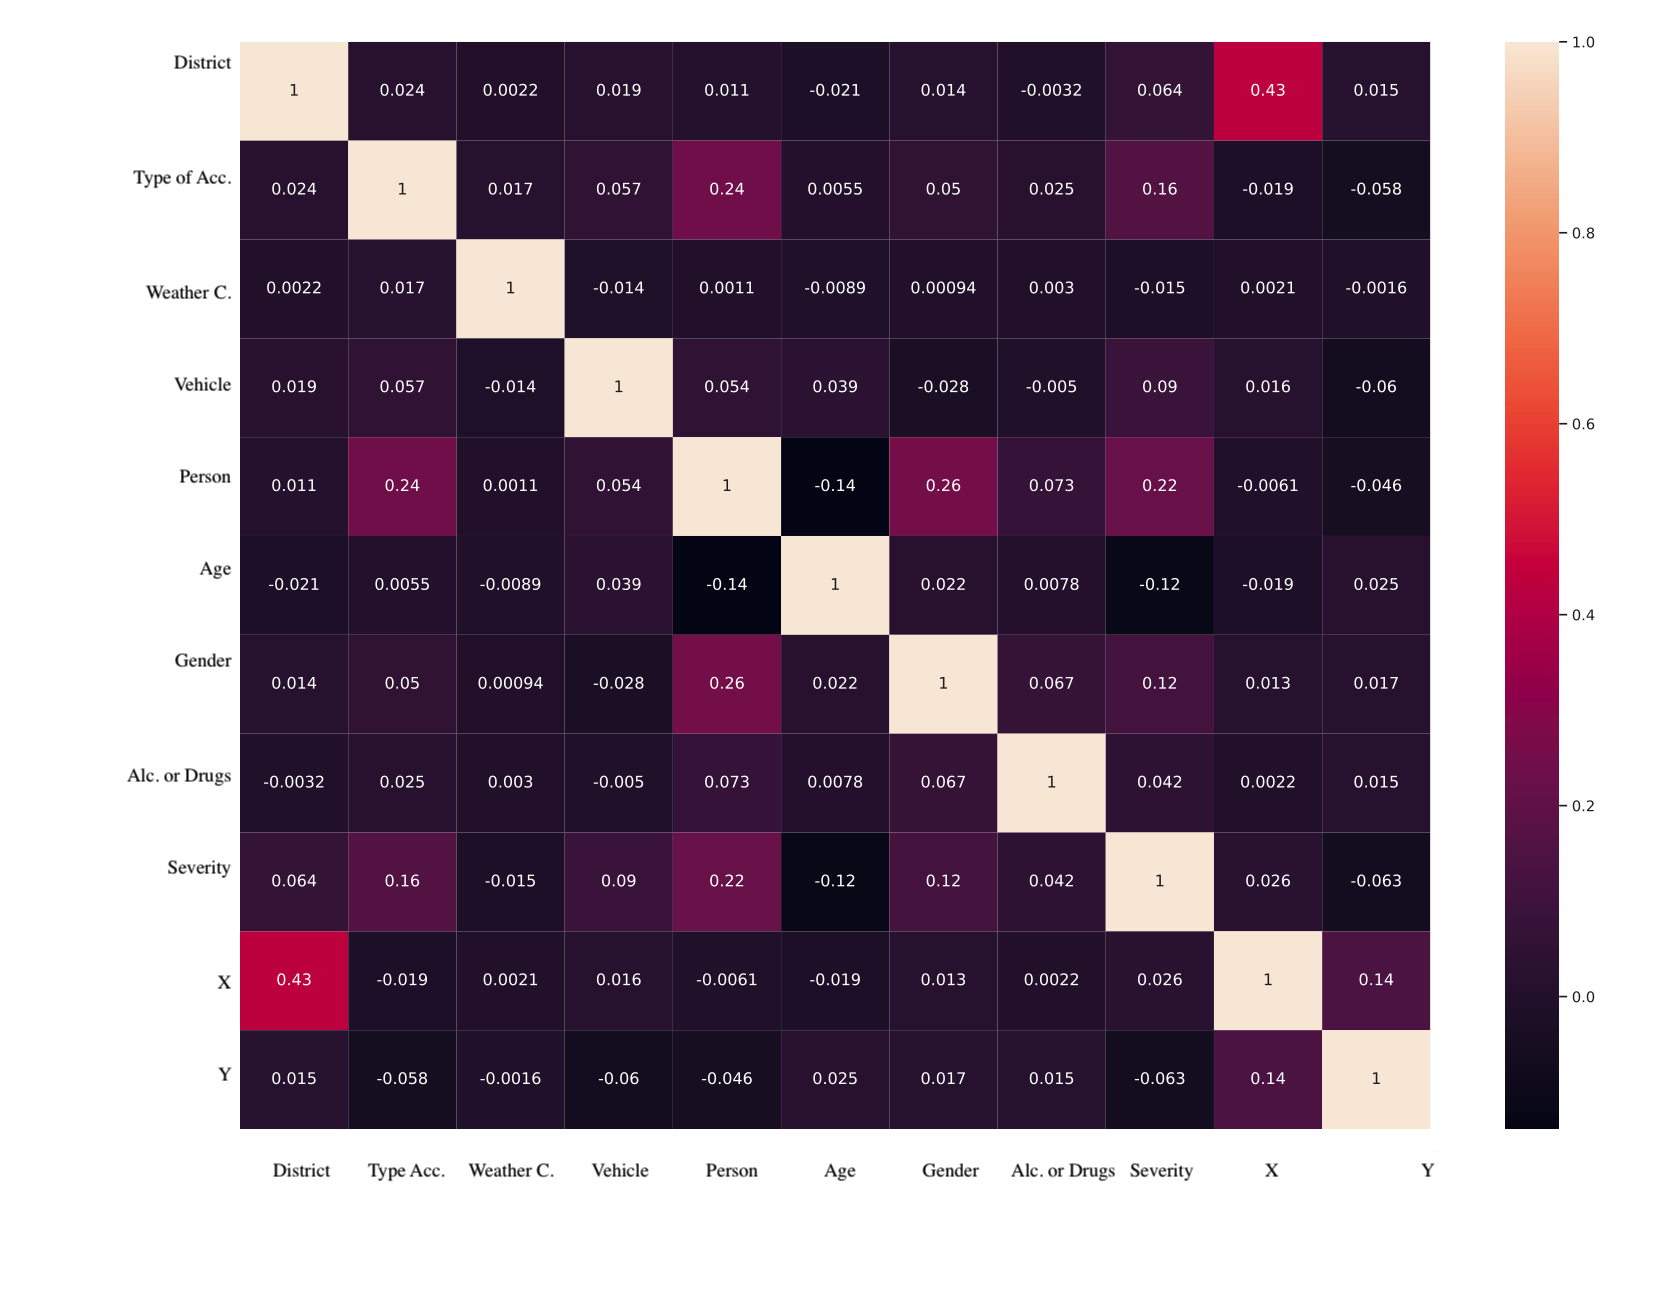
\includegraphics[width=12cm]{Figures/1stPaper/CorrelationMatrix.png}
	\caption{Matriz de correlación entre las variables del conjunto de datos de Madrid}
	\label{CorrelationMatrix}
\end{figure}


\subsection*{Discretización}

Una vez se disponían de los datos refinados y las características adecuadas seleccionadas, era necesario transformar los valores para hacerlos interpretables por los modelos. Este proceso se hizo mediante la asignación de valores numéricos a cada una de las variables cualitativas del dataset en función de la fuerza que representaban los valores de cada característica. Por otra parte, las variables originales \textit{Positivo en Drogas} y \textit{Positivo en Alcohol} se unieron en una nueva característica \textit{Alcohol o Drogas}, con el objetivo de recoger esta información en un único campo y no descartar registros que presentaban valores nulos en ambas columnas. En la Tabla \ref{TransformacionDatosTabla} se muestra la discretización realizada para cada una de las variables.

\textcolor{purple}{Si pones dos columnas en vez de cuatro quedará mejor}
%%%%%%%%%%%%%%%%%%%%%%%%%%%%%%%%%%%%%%%%%%%%%%%%%%%%%%%%%%%%%%%%%%%%%%%%%%%%%%%%%

\begin{table}[H]
	\centering
	\renewcommand{\arraystretch}{1.2}
	\small
	
	\begin{tabular}{|c|l|c|l|}\hline
		\textbf{Característica} & \textbf{Tipificación} & \textbf{Característica} & \textbf{Tipificación} \\ \hline
		\multirow{3}{*}{\textbf{Gravedad}} & 0: Leve (\textit{1, 2, 5, 6, 7}) & \multirow{2}{*}{Tiempo} & 1: Noche (\textit{6 PM - 6 AM}) \\
		& 1: Grave (\textit{3}) & & 2: Día (\textit{6 AM - 6 PM}) \\ \cline{3-4}
		& 2: Fatal (\textit{4}) & Distrito & En base al orden de aparición \\ \hline
		\multirow{1}{*}{X} & Posición Coordenada UTM X & \multirow{12}{*}{Tipo de Accidente} & 1: Colisión frontal \\ \cline{1-2}
		\multirow{1}{*}{Y} & Posición Coordenada UTM Y & & 2: Colisión trasera \\ \cline{1-2}
		\multirow{9}{*}{Tipo de Carretera} & 1: Estacionamiento & & 3: Choque lateral \\
		& 2: Aeropuerto & & 4: Colisión contra obstáculo fijo \\
		& 3: Parque & & 5: Choque en cadena \\
		& 4: Túnel & & 6: Atropello a peatón \\
		& 5: Zona industrial & & 7: Colisión frontal \\
		& 6: Pista & & 8: Otro \\
		& 7: Rotonda & & 9: Salida de la carretera \\
		& 8: Glorieta & & 10: Vuelco de vehículo \\
		& 9: Puerta & & 11: Atropello a animal \\
		& 10: Puente & & 12: Caída \\ \hline
		\multirow{7}{*}{Condiciones Meteorológicas} & 1: Soleado & \multirow{1}{*}{Vehículo} & En base al orden de aparición \\ \cline{3-4}
		& 2: Nublado & \multirow{3}{*}{Persona} & 1: Conductor \\
		& 3: Lluvia ligera & & 2: Pasajero \\
		& 4: Lluvia intensa & & 3: Peatón \\ \cline{3-4}
		& 5: Granizo & \multirow{5}{*}{Edad} & 1: Menos de 18 años \\
		& 6: Nevando & & 2: De 18 a 25 años \\
		& 7: Desconocido & & 3: De 25 a 65 años \\ \cline{1-2}
		\multirow{3}{*}{Género} & 1: Masculino & & 4: Más de 65 años \\
		& 2: Femenino & & 5: Desconocida \\ \cline{3-4}
		& 3: Desconocido & \multirow{1}{*}{Alcohol o Drogas} & 1: Sí / 2: No\\ \hline
	\end{tabular}
	
	\caption{Asignación numérica de las variables del conjunto de datos}
	\label{TransformacionDatosTabla}
\end{table}

%%%%%%%%%%%%%%%%%%%%%%%%%%%%%%%%%%%%%%%%%%%%%%%%%%%%%%%%%%%%%%%%%%%%%%%%%%%%%%%%%

\subsection*{División de datos}


Como es habitual en el diseño de los modelos predictivos, es común dividir los datos en subconjuntos para el aprendizaje de los modelos y su evaluación real sobre registros que nunca ha visto. Del total de muestras resultantes del proceso de filtrado ($65\,158$) se asignan el 80\% de ellas para el conjunto de entrenamiento ($54\,211$), resultando en $53\,213$ accidentes leves, $984$ graves y $50$ fatales. El $20\%$ de los datos restantes se asignaron al conjunto validación o test ($10\,911$), concretamente $10\,640$ accidentes leves, $256$ graves y $15$ fatales.

\subsection*{Normalización}

% \textcolor{red}{\textbf{Luis: Inquietud} Si pongo un ejemplo de normalización random en eta sección, qué pondríamos en resultados GTAAF en esta fase para no repetirnos? Veo lagunas}

% \textcolor{orange}{\textbf{Luis: Propuesta} Lo mencionamos en el resampling como una última frase y listo?}
% \textcolor{purple}{Pon un ejemplo random aquí y en GTAAF se comenta que la normalización es idéntica. Además, deberías poner el rango de normalización}

Una vez aplicado el proceso de limpieza de datos y elección de características del dataset, se aplica la normalización en base a la técnica \textit{Z-Score}, que transformará los datos a una distribución normal con media 0 y desviación 1 de cada valor. Este proceso se aplica para cada una de las muestras de tal forma que la dimensión de los datos quede bajo la misma magnitud, para poder ser  interpretarse eficientemente por los modelos. Una vez se dispone de todos los datos normalizados, pueden ser utilizados para el entrenamiento de cualquier modelo predictivo.


\subsection*{Resampling}


En el punto en el que se disponían de los datos normalizados e interpretables por los modelos, se analizó la distribución final de los datos de entrenamiento en base a la clase a predecir, la gravedad del accidente. Atendiendo a los registros resultantes (Leve, Grave y Fatal), se pudo observar que el conjunto de datos estaba claramente desbalanceado. Se disponían de $53\,213$ accidentes leves, $984$ graves y $50$ fatales. Esto, como se ha comentado en la sección \ref{SOAT_RESAMPLING}, se convierte en un problema para los modelos de clasificación, ya que en estos casos tienden a predecir las nuevas muestras como aquellas que pertenecen a la clase mayoritaria. Para paliar este problema se aplicó la técnica de remuestreo \textit{Borderline SMOTE-II}, con el objetivo de generar más muestras de accidentes pertenecientes a clases minoritarias (Grave y Fatal) hasta llegar a la mayoritaria (Leves), evitando que el modelo se sobreajuste. Una vez aplicado el algoritmo, se disponen de $53\,213$ muestras de la clase leve, $53\,213$ de la clase grave y $53\,213$ de la clase fatal, haciendo un total de $159\,639$ registros en el nuevo conjunto de datos de entrenamiento balanceado.



\subsection*{Categorización}

Como se ha comentado en secciones anteriores, las redes neuronales convolucionales aprenden patrones utilizando matrices como datos de entrada. Así pues, como se disponen de datos tabulares, se hace necesario transformarlos en matrices.

Uno de los requisitos de esta transformación era asignar cada característica a una categoría del dataset. Sobre este conjunto de datos de Madrid, las variables eran asignadas a $5$ categorías en base a la información de la que se disponía: (1) Características del accidente, (2) Condiciones de la carretera, (3) Condiciones meteorológicas, (4) Características del vehículo y (5) Características del conductor. En la Tabla \ref{JC} se observa la categorización de cada característica en función de la información que describen.

% \textcolor{red}{\textbf{Luis: Comentario} Exponer la categorización no me termina de cuadrar aquí, principalmente porque en el siguiente (GTAAF) esto se pone en la descripción de los datos. A lo mejor no está mal dejarlo como está... Porque así el lector le daría más importancia a la categorización en el modelo GTAAF, porque aparece lo primero. No sé, también es verdad que si lo dejamos así queda un poco caótico a la hora de comparar la metodología preliminar y la GTAAF. Siento el rollo, hay alguna opinión? :-(}

% \textcolor{purple}{Lo dejamos así y cuando se explique GTAAF hay que decir que esta categorización es fundamental para generalizar el modelo por eso se explica en la descripciónd e los datos.}


% \textcolor{red}{\textbf{Luis: CUIDADO} En el paper 1 en esta tabla se pone severidad dentro de accidente... y no es el único sitio. Es posible solicitar correcciones del otro paper?}
% \textcolor{green}{MANU: se que se puede de alguna forma, pero nunca lo he hecho...}

\begin{table}[H]
	\centering
	
	\begin{tabular}{ |c|c| }
		\hline
		\textbf{Categoría} & \textbf{Característica} \\
		\hline
		\hline
		\multirow{5}{*}{Accidente} & X \\
		& Y \\
		& Hora \\
		& Tipo de accidente \\
		& Vehículos implicados \\
		\hline
		\hline
		\multirow{2}{*}{Carretera} & Tipo de carretera \\
		& Distrito \\
		\hline
		\hline
		Clima & Condiciones climáticas \\
		\hline
		\hline
		Vehículo & Tipo de Vehículo \\
		\hline
		\hline
		\multirow{4}{*}{Conductor}  & Tipo de Persona \\
		& Género \\
		& Edad \\
		& Alcohol o Drogas \\
		\hline
		\hline
	\end{tabular}
	
	\caption{Clasificación de características (variables del conjunto de datos) en categorías. Modelo Preeliminar}
	\label{JC}
\end{table}



\subsection*{Algoritmo Genético}

% \textcolor{red}{\textbf{Luis: CUIDADO} En el paper 1 dijimos que se optimizaron cinco hiperparámetros del XGBoost cuando esto es falso. Aquí he puesto la realidad. Qué hacemos?}

% \textcolor{purple}{Déjalo como está, no creo que nadie se mire el paper 1 para comparar. Si te preguntan en el tribunal, puedes decir que al principio se optimizaron 5 pero que el resultado de 2 de ellos siempre era el mismo, con lo que se decidió optimizar solo 3}

En este punto, se analiza la optimización de los hiperparámetros del algoritmo \textit{XGBoost} a través del algoritmo genético mediante la maximización de la métrica \textit{F1-Score} de los datos de entrenamiento. Los hiperparámetros del algoritmo \textit{XGBoost} a optimizar fueron: profundidad máxima del árbol, peso mínimo de los hijos y el ratio de aprendizaje. El algoritmo genético se configuró para optimizar esta función durante $80$ generaciones, con un máximo de $40$ individuos en la población y los $10$ mejores en cada iteración eran seleccionados para reproducirse mediante una estrategia de cruce aleatorio.

La figura \ref{EvolucionHiperparametrosImage} muestra la evolución de  los tres hiperparámetros del \textit{XGBoost} a lo largo de las generaciones. Como se puede observar, los hiperparámetros toman distintos valores en función del mejor individuo evaluado en la población en cada etapa, estos hiperparámetros convergían aproximadamente en la iteración $42$, donde no se observaron incrementos en este métrica a partir de esta generación.

\begin{figure}[H]
	\centering
	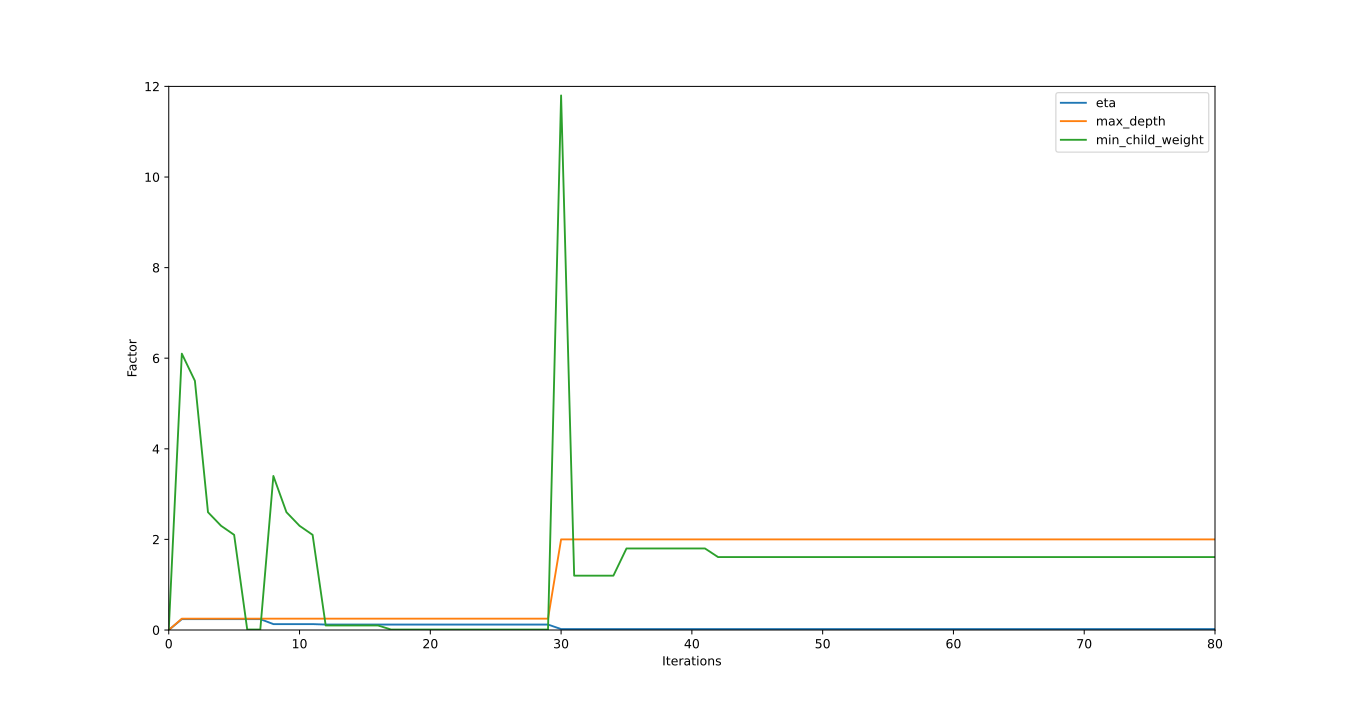
\includegraphics[width=14cm]{Figures/1stPaper/EvolutionH.png}
	\caption{Evolución de los hiperparámetros del \textit{XGBoost} a lo largo de las generaciones}
	\label{EvolucionHiperparametrosImage}
\end{figure}

En la tabla \ref{BestGASolutionTable} se observa el valor tomado por el mejor individuo resultante de la ejecución de las distintas generaciones para cada uno de los hiperparámetros del \textit{XGBoost}. 

%%%%%%%%%%%%%%%%%%%%%%%%%%%%%%%%%%%%%%%%%%%%%%%%%%%%%%%%%%%%%%%%%%%%%%%%%%%%%%%%%
\begin{table}[h]
	\caption{Valores optimizados de los parámetros del \textit{XGBoost} después de aplicar el algoritmo genético del modelo preliminar}
	\centering
	\begin{tabular}{ |c|c| } 
		\hline
		\textbf{Hiperparámetro} & \textbf{Valor}\\
		\hline
		Profundidad Máxima & 2 \\
		Peso Mínimo de Hijos & 1.6 \\ 
		ETA & 0.007 \\
		\hline
	\end{tabular}

	\label{BestGASolutionTable}
\end{table}
%%%%%%%%%%%%%%%%%%%%%%%%%%%%%%%%%%%%%%%%%%%%%%%%%%%%%%%%%%%%%%%%%%%%%%%%%%%%%%%%%

%\underline{Pesos de categorías}

Con la configuración de hiperparámetros mostrada en la Tabla \ref{BestGASolutionTable} se entrena el algoritmo \textit{XGBoost} para obtener el peso de todas las  características del conjunto de datos. Así, en la Tabla \ref{1stPaperWeightsFinalCharacteristics} se muestra el peso asignado a cada una de las características individuales, donde la columna peso de la Categoría muestra el peso de cada categoría como suma de los peso de cada una de las características individuales que la componen.

% \textcolor{red}{\textbf{Luis: CUIDADO} En el paper 1 en esta tabla se pone severidad dentro de accidente... y no es el único sitio. Es posible solicitar correcciones del otro paper?}

%%%%%%%%%%%%%%%%%%%%%%%%%%%%%%%%%%%%%%%%%%%%%%%%%%%%%%%%%%%%%%%%%%%%%%%%%%%%%%%%%
\begin{table}[ht]
	\caption{Ejemplo con los pesos de todas las características estudiadas, así como los pesos de las cinco categorías}
	\centering
	\begin{tabular}{ |c|c||c|c| }
		\hline
		\textbf{Categoría} & \textbf{Peso} & \textbf{Característica} & \textbf{Peso}\\
		\hline
		\hline
		\multirow{5}{*}{Accidente}   & \multirow{5}{*}{0.299} & Coordenada X & 0.071\\
		&  & Coordenada Y  & 0.066\\
		&  & Hora & 0.055\\
		&  & Tipo de accidente  & 0.051\\
		&  & Vehículos implicados & 0.057\\
		\hline
		
		\multirow{2}{*}{Carretera} & \multirow{2}{*}{0.187} & Distrito  & 0.059\\      
		&  & Tipo de Carretera & 0.127\\
		\hline
		
		\multirow{1}{*}{Clima}  & \multirow{1}{*}{0.050}  & Condiciones Climáticas  & 0.050\\
		\hline
		
		\multirow{1}{*}{Vehículo}  & \multirow{1}{*}{0.070} & Tipo de Vehículo  & 0.070\\
		\hline
		
		\multirow{4}{*}{Conductor}   & \multirow{4}{*}{0.394} & Tipo de Persona & 0.177\\
		&      & Género      & 0.111\\
		&      & Edad      & 0.050\\
		&      & Alcohol o Drogas  & 0.056\\
		\hline
		
	\end{tabular}

	\label{1stPaperWeightsFinalCharacteristics}
\end{table}

\subsection*{Construcción de matrices}


Una vez se disponían de las características y categorías evaluadas, se aplicaba el proceso de asignación de posiciones de cada característica a las respectivas coordenadas dentro de la matriz, aplicando el algoritmo de construcción de matrices.

En la Tabla \ref{ProcesoMatriz:Array} se observa un ejemplo de un registro transformado a formato matricial una vez se ha aplicado el algoritmo de construcción haciendo uso de la importancia de las características de la tabla \ref{1stPaperWeightsFinalCharacteristics}. Igualmente, en la figura \ref{ProcesoMatriz:VisualizacionDeMatriz}, se observa la representación en imagen de escala de grises de dicha matriz.


\begin{table}[H]
	\caption{Matriz resultante tras la transformación de un registro a formato matricial. Las filas representan las categorías y las columnas las características que la componen, ordenadas en función de los pesos mediante el criterio presentado en la sección \ref{METODOLOGIA_MODELO_PRELIMINAR}}
	\begin{center}
		\begin{tabular}{|c|c|c|c|c|}
			\hline
			$0.0$ & $0.0$ &  $-0.1621$  & $0.0$ & $0.0$\\
			$1.2548$ & $0.0081$ &  $-0.0524$  & $-1.4528$ & $-1.4591$\\
			$0.2129$ & $-0.7004$ &  $-0.5316$  & $0.1488$ & $0.0$\\
			$0.0$ & $-0.0297$ &  $0.4597$  & $0.0$ & $0.0$\\
			$0.0$ & $0.0$ &  $-0.2508$  & $0.0$ & $0.0$\\
			\hline
		\end{tabular}
	\end{center}

	\label{ProcesoMatriz:Array}
\end{table}

\begin{figure}[H]
	\centering
	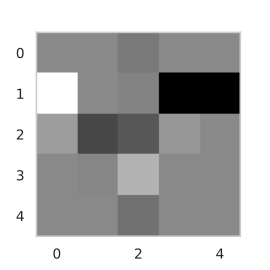
\includegraphics[width=6cm]{Figures/TFM/accidente_fatal.png}
	\caption{Imagen de la matriz en escala de grises.}
	\label{ProcesoMatriz:VisualizacionDeMatriz}
\end{figure}


%\begin{figure}[H]
%   \centering
%   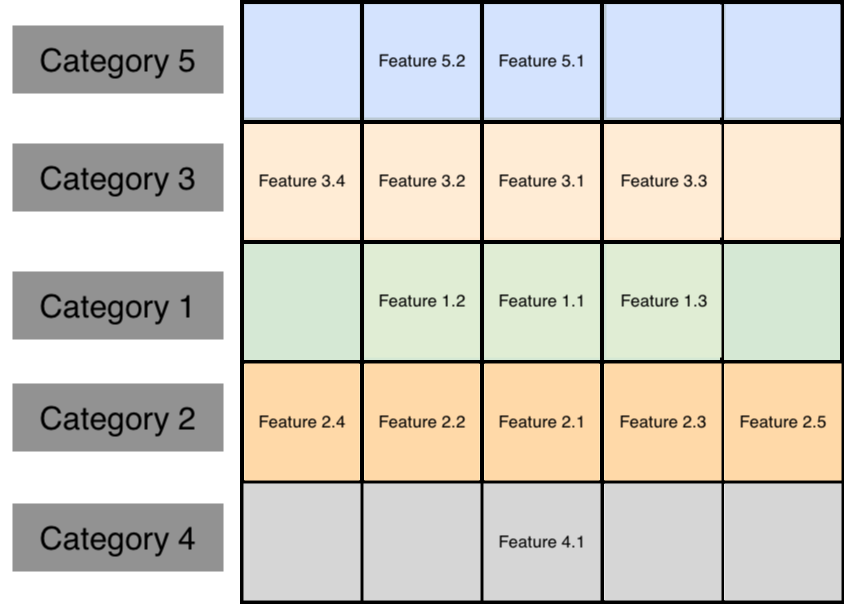
\includegraphics[width=10cm]{Figures/1stPaper/FV2I.png}
%   \caption{Example of positioning the elements in a matrix. Categories are assigned in rows based on their weight, and Features are assigned in the columns of the corresponding category based on their weight.}
%   \label{FV2IExample}
%\end{figure}

\subsection*{Entrenamientos}

Una vez que las matrices han sido construidas, se describe la red convolucional utilizada en el modelo propuesto. En esta sección se presenta la información resultante de los entrenamientos realizados para los dos modelos convolucionales, de una y dos dimensiones, sobre los que trabaja la metodología preliminar. De esta forma se analizará la evolución de la función de pérdida en cada uno de estos modelos. Ambos fueron entrenados con $100$ épocas, al analizar la evolución del entrenamiento de la red convolucional unidimensional (CNN-1D), se puedo verificar que la puntuación \textit{F1-Score} de entrenamiento incrementaba ínfimamente a lo largo de las épocas, sufriendo además altibajos sobre el conjunto de validación a medida que el modelo se entrenaba, comenzando inicialmente con un valor de entrenamiento inferior a $0.58$ y llegando hasta $0.68$, mostrando poca capacidad de aprendizaje y generalización ante nuevas muestras.

Por otro lado, sobre el modelo convolucional bidimensional (CNN-2D) observó que la tendencia de la función de pérdida en el conjunto de datos de entrenamiento era más estable. Se pudo comprobar cómo la red, en la primera ejecución, comenzaba con una puntuación \textit{F1-Score} de $0.62$ hasta alcanzar $0.78$ en la iteración $100$, por lo que se puedo deducir que esta red lograba un mejor rendimiento en el conjunto de entrenamiento en comparación con la red convolucional unidimensional, sufriendo menos altibajos en el conjunto de validación.


\subsection*{Evaluación}

% \textcolor{red}{\textbf{Luis: quitaría incluso el análisis de los datos de entrenamiento}}

Para evaluar el rendimiento del modelo preeliminar, se realizó una comparación con tres modelos del estado del arte, \textit{Gaussian Naive Bayes (GNB), Support Vector Classifier (SVC)} y \textit{K-Nearest Neighbor (KNN)}. En esta sección se utilizarán las métricas obtenidas tras la ejecución de los cinco modelos sobre el conjunto de datos de test (\textit{CNN-1D, CNN-2D, GNB, SVC} y \textit{KNN}).

Las Tablas \ref{ClassificationReportCNN:TrainCNN} y \ref{ClassificationReportCNN:TestCNN} detallan las métricas resultantes de la clasificación de las redes para los conjuntos de entrenamiento y test respectivamente. Se observó que, para el conjunto de entrenamiento, el modelo CNN-1D obtenía un mejor \textit{F1-Score} en la clasificación de todas las clases de accidentes en comparación con la red CNN-2D. Sin embargo, al analizar las métricas de los datos de test, el modelo que presentaba mejor \textit{F1-Score} para accidentes leves y graves era el CNN-2D, con $0.950$ y $0.148$ respectivamente, mientras que en accidentes fatales ambas redes ofrecían el mismo rendimiento con un $0.004$ de \textit{F1-Score}.

\begin{table}[H]
	\caption{Métricas sobre el conjunto de entrenamiento para los modelos CNN-1D y CNN-2D}
	\begin{center}
		\begin{tabular}{|c||c|c|c||c|c|c|}
			\hline
			\multicolumn{1}{ |c|| }{} & \multicolumn{3}{ |c|| }{\textbf{CNN-1D}} & \multicolumn{3}{ |c| }{\textbf{CNN-2D}} \\ \hline
			\textbf{Métrica/Gravedad} & Leve & Grave & Fatal & Leve & Grave & Fatal
			\\ \hline \hline 
			Precision & 0.701 & 0.696 & 0.754 & 0.488 & 0.646 & 0.966 \\ \hline 
			Recall & 0.724 & 0.523 & 0.917 & 0.974 & 0.299 & 0.524\\ \hline 
			F1-score & 0.712 & 0.597 & 0.828 & 0.650 & 0.409 & 0.679\\ \hline 
		\end{tabular}
	\end{center}

	\label{ClassificationReportCNN:TrainCNN}
\end{table}

\begin{table}[H]
	\caption{Métricas sobre el conjunto de test para los modelos CNN-1D y CNN-2D}
	\begin{center}
		\begin{tabular}{|c||c|c|c||c|c|c|}
			\hline
			\multicolumn{1}{ |c|| }{} & \multicolumn{3}{ |c|| }{\textbf{CNN-1D}} & \multicolumn{3}{ |c| }{\textbf{CNN-2D}} \\ \hline
			\textbf{Métrica/Gravedad} & Leve & Grave & Fatal & Leve & Grave & Fatal
			\\ \hline \hline 
			Precision & 0.984 & 0.031 & 0.002 & 0.982 & 0.097 & 0.002\\ \hline 
			Recall & 0.429 & 0.394 & 0.333 & 0.919 & 0.313 & 0.1\\ \hline 
			F1-score & 0.596 & 0.058 & 0.004 & 0.950 & 0.148 & 0.004\\ \hline 
		\end{tabular}
	\end{center}

	\label{ClassificationReportCNN:TestCNN}
\end{table}

% \textcolor{red}{\textbf{Luis: Percepción} me da la sensación de que hay mucho contenido aquí. La forma de exponer los resultados (primero los de las CNNs y luego los modelos del estado del arte) provoca que esto sea muy largo cuando en mi opinión, estos resultados no tienen mucha importancia. Lo reestructuramos o qué pensais?}

% \textcolor{purple}{Jose: Tienes razón, se me está haciendo un poco pesado de leer, lo que significa que deberíamos reducirlo. ¿Quitamos lo referente a las matrices de confusión y lo centramos en los resultados del F1-score?}

% \textcolor{orange}{Luis: Me parece buena idea, he quitado lo relativo a las matrices. Además creo que deberíamos reducir todo lo referente a los resultados preliminares..}

% La Figura \ref{ConfusionMatricesImages} muestra las matrices de confusión para los conjuntos de entrenamiento y test de ambos modelos, donde se pueden analizar las tendencias predictivas. Para los datos de entrenamiento de CNN-2D, tendía a una mayor propensión de predecir observaciones como accidentes leves en comparación con la red CNN-1D. Esto provocaba que la CNN-1D clasificase correctamente más accidentes graves y fatales. Para el conjunto de datos de test, la red CNN-2D clasificaba más observaciones como accidentes leves que el modelo CNN-1D, prediciendo menos accidentes graves pero con mayor confianza.

% %%%%%%%%%%%%%%%%%%%%%%%%%%%%%%%%%%%%%%%%%%%%%%%%
% \begin{figure}[H]
	%     \centering
	%     \subfigure[Training CNN-1D]{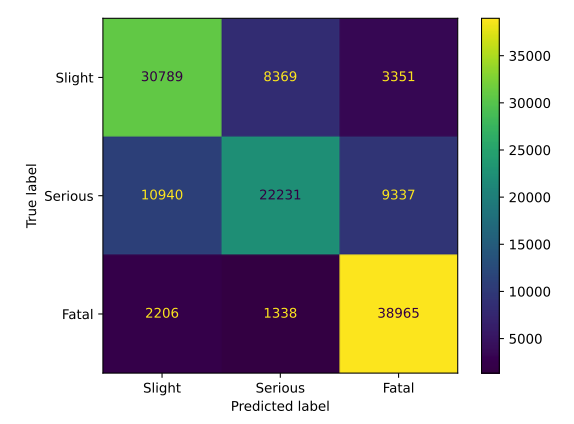
\includegraphics[width=60mm]{Figures/1stPaper/1DConfusionMatrixTrain}}
	%     \subfigure[Training CNN-2D]{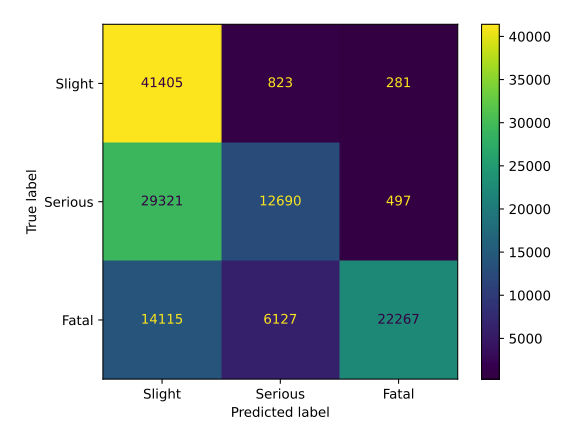
\includegraphics[width=60mm]{Figures/1stPaper/2DConfusionMatrixTrain}}
	%     \subfigure[Test CNN-1D]{\includegraphics[width=60mm]{Figures/1stPaper/1DConfusionMatrixTest}}
	%     \subfigure[Test  CNN-2D]{\includegraphics[width=60mm]{Figures/1stPaper/Diagrama sin título.drawio}}
	%     \caption{Matrices de confusión de entrenamiento y test para las redes neuronales convolucionales.}
	%     \label{ConfusionMatricesImages}
	% \end{figure}
% %%%%%%%%%%%%%%%%%%%%%%%%%%%%%%%%%%%%%%%%%%%%%%%%


La información con la que se evalúan los modelos, es decir, las métricas de clasificación resultantes para el conjunto de test se muestran en la Tabla \ref{ClassificationReportCNN:Test} para cada una de las clases predichas. Como se puede ver en esta tabla, el modelo \textit{KNN} obtiene mejores resultados en todas las medidas de todas las clases, excepto en \textit{Recall} en accidentes graves, donde el \textit{GNB} es un ligeramente mejor.

Si analizamos la métrica de \textit{Precision} en los cinco modelos comparados, se puede observar que el modelo que presenta el mejor promedio para las clases de accidentes leves es la Red Neuronal Convolucional 1D (CNN-1D) con $0.984$, seguida por la Red Neuronal Convolucional 2D (CNN-2D) y el modelo \textit{KNN} con $0.982$. Además, la CNN-2D también ofrece la mejor métrica para accidentes graves, $0.097$, con una gran diferencia respecto al modelo que le sigue, \textit{KNN} con $0.042$. En cuanto a los accidentes fatales, ambos modelos CNN-1D y CNN-2D tienen un valor similar, obteniendo $0.002$.

Con respecto a la métrica de \textit{Recall}, el mejor promedio para las clases de accidentes leves es la Red Neuronal Convolucional 2D (CNN-2D) con $0.919$, seguida por el modelo \textit{KNN} con $0.689$. Además, el modelo \textit{GNB} ofrece la mejor métrica para accidentes graves, $0.699$. En accidentes fatales, CNN-2D presenta el mejor valor con $0.1$.

Es necesario señalar que el \textit{F1-score} es una forma de combinar las métricas de \textit{Precision} y \textit{Recall}, y se define como la media armónica de ambas. Teniendo esto en cuenta, analizando el \textit{F1-Score} de los reportes, el modelo que presenta el mejor promedio para las clases de accidentes leves es la red CNN-2D, alcanzando $0.950$, muy por encima del siguiente modelo \textit{KNN}, que ofrece un valor de $0.810$. Además, la CNN-2D también ofrece la mejor métrica para accidentes graves, $0.148$, alcanzando el doble de rendimiento en comparación con el modelo que le sigue, \textit{KNN} con $0.076$. En cuanto a los accidentes fatales, los modelos con mejor clasificación son tanto la CNN-1D como la CNN-2D, obteniendo $0.004$, el doble que \textit{KNN}, que son los siguientes mejores modelos en esta clase con $0.002$.

Podemos concluir que el modelo preliminar propuesto, basado en redes neuronales convolucionales (CNN-1D y CNN-2D), presentaba mejores predicciones con respecto a la métrica \textit{F1-score}, aunque con gran potencial de mejora.

\begin{table}[H]
	\caption{Métricas de clasificación sobre el conjunto de test de los modelos \textit{GNB}, \textit{SVC} y \textit{KNN} en comparación con el modelo preliminar.}
	\begin{center}
		\begin{tabular}{|c||c|c|c|}
			\hline
			 \multicolumn{4}{ |c| }{\textbf{GNB}} \\
			  \hline \hline
			\textbf{Métrica/Gravedad} & Leve & Grave & Fatal \\  \hline 
			Precision & 0.980 & 0.025 & 0  \\ \hline 
			Recall & 0.369 & 0.699 & 0  \\ \hline 
			F1-score & 0.536 & 0.048 & 0 \\ \hline
			 \multicolumn{4}{ c }{} \\ 
			 
			 \hline
			 \multicolumn{4}{ |c| }{\textbf{SVC}} \\ 
			 \hline \hline
			\textbf{Métrica/Gravedad} & Leve & Grave & Fatal \\  \hline 
			Precision  & 0.979 & 0.029 & 0  \\ \hline 
			Recall  & 0.644 & 0.411 & 0  \\ \hline 
			F1-score & 0.777 & 0.054 & 0 \\ \hline
			\multicolumn{4}{ c }{} \\ 
			
			\hline
			\multicolumn{4}{ |c| }{\textbf{KNN}} \\ 
			\hline \hline
			\textbf{Métrica/Gravedad} & Leve & Grave & Fatal \\  \hline 
			Precision & 0.982 & 0.042 & 0.001 \\ \hline 
			Recall & 0.689 & 0.382 & 0.067 \\ \hline 
			F1-score  & 0.810 & 0.076 & 0.002\\ \hline 
		\end{tabular}
	\end{center}
	\label{ClassificationReportCNN:Test}
\end{table}


% \textcolor{purple}{Jose: ¿Quitamos lo de las matrices de confusión en este apartado?}

% \textcolor{orange}{Luis: Quitado}

% La Figura \ref{ClassificationReportCNN:Test} muestra las matrices de confusión aplicadas al conjunto de prueba, presentando una representación visual de las métricas de clasificación. Esto permite abordar el hecho de que los modelos GNB y SVC no clasifican correctamente ninguna de las observaciones de accidentes fatales, mientras que KNN clasifica una. En cuanto a los accidentes leves, el modelo CNN-2D es el que clasifica correctamente el mayor número, al igual que en los accidentes graves. Esto se debe a la naturaleza de las redes aplicadas a la complejidad del problema, cada una de ellas encuentra patrones diferentes según los mapas característicos resultantes de las convoluciones de cada red.


% % \textcolor{red}{\textbf{Luis: CUIDADO} Cuidado con el CNN-2D test, el nº de muestras de accidentes fatales no concuerda con el resto. Sigo sin saber cómo nos aprobaron ese paper.}

% %%%%%%%%%%%%%%%%%%%%%%%%%%%%%%%%%%%%%%%%%%%%%%%%
% \begin{figure}[H]
	% \centering
	% %\subfigure[Training CNN-1D]{\includegraphics[width=70mm]{Figures/1DConfusionMatrixTest}}
	% %\subfigure[Training CNN-2D]{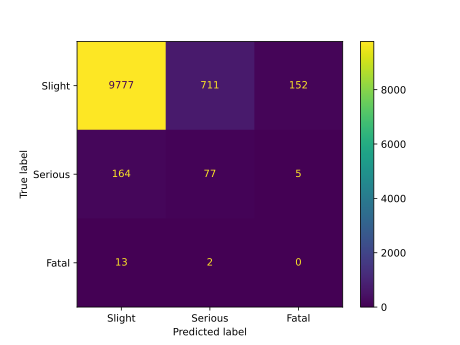
\includegraphics[width=70mm]{Figures/2DConfusionMatrixTest}}
	% \subfigure[Test GNB]{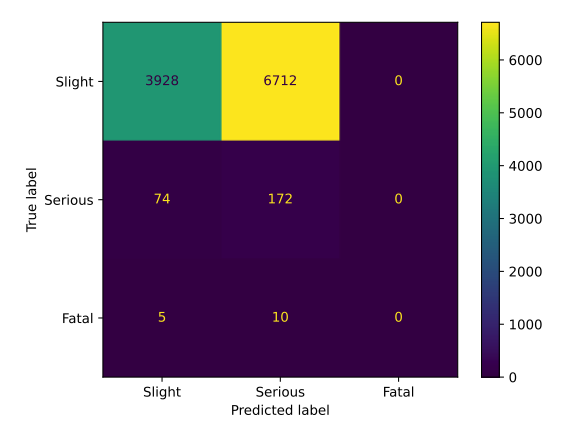
\includegraphics[width=60mm]{Figures/1stPaper/NBConfusionMatrixTest.png}}
	% \subfigure[Test KNN]{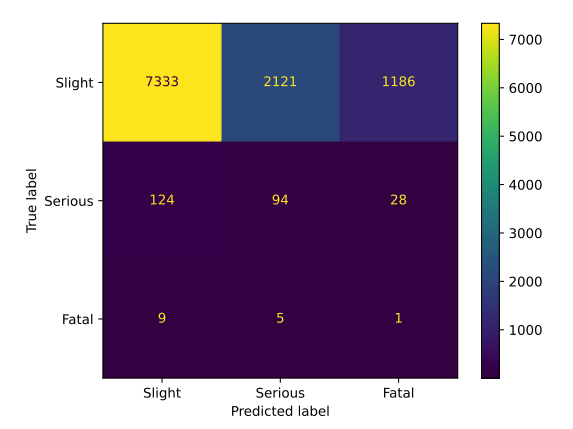
\includegraphics[width=60mm]{Figures/1stPaper/KNNConfusionMatrixTest.png}}
	% \subfigure[Test SVC]{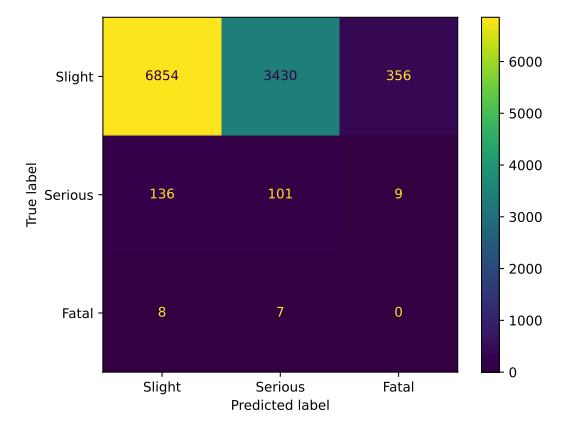
\includegraphics[width=60mm]{Figures/1stPaper/SVCConfusionMatrixTest.png}}
	% \caption{Matrices de confusión aplicadas para el conjunto de test de los modelos GNB, SVC y KNN.}
	% \label{ConfusionMatrixCNNImages}
	% \end{figure}
% %%%%%%%%%%%%%%%%%%%%%%%%%%%%%%%%%%%%%%%%%%%%%%%%

% Como se puede observar en los resultados de los experimentos, las dos arquitecturas convolucionales propuestas superan al resto de los modelos de referencia para cada una de las clases de accidentes (Leves, Graves y Fatales). La ventaja de contar con estas dos nuevas arquitecturas es que cada una de ellas funciona mejor según el tipo de clase que se va a predecir. Esto permite el diseño de un sistema en el cual las dos redes entrenadas se utilicen para combinar sus resultados, de manera que la red CNN-1D se usaría para predecir accidentes leves y fatales, mientras que la red CNN-2D clasificaría accidentes graves.

\subsection*{Discusión de resultados del modelo preliminar}

% \textcolor{red}{\textbf{Luis: } esto es realmente lo mismo que la introducción al modelo GTAAF pero más justificado en base al análisis de resultados, no sé si estaría bien repetirse.}

% \textcolor{purple}{\textbf{Jose: Aquí pondría esto}}

Analizando los resultados finales de este modelo preliminar se propusieron una serie de mejoras a desarrollar para crear un modelo general en la gravedad de los accidentes de tráfico, aportando así un posible valor a las administraciones públicas para asignar recursos médicos en los accidentes de tráfico. En primer lugar, se detectó que la decisión de disgregar la clasificación de la gravedad de los accidentes en tres clases provocaba un efecto conflictivo en la clasificación de los modelos debido a que dos de las clases en las que se dividía la gravedad de los accidentes eran minoritarias, lo que penalizaba el aprendizaje del modelo. Por otra lado, al intentar generalizar el modelo, la adaptación de la metodología para poder aplicarla en cualquier conjunto de datos era prioritaria. De esta forma, cualquier información que pudiese ser relevante en la predicción de la gravedad de los accidentes, orientado a la falta de disponibilidad de datos en cada región, debería ser añadida. Finalmente se comprobó que había datos ya existentes de los que se podían sacar más características importantes. Por ejemplo, la hora del accidente no estaba representada debido a su naturaleza cíclica. Todos estas debilidades hicieron necesario la implantación de soluciones que aportaran generalidad al modelo definitivo.

% \textcolor{purple}{\textbf{Jose: Los siguientes párrafos los pasaría al modelo definitivo, al principio de la sección siguiente}}


%%%%%%%%%%%%%%%%%%%%%%%%%%%%%%%%%%%%%%%%%%%%%%%%%%%%%%%%%%%%%%%%%%%%%%%%%%%%%%%%%%%%%%%%%%%%%%%%%%%%%%%%%%%%%%%%%%%%%%%%%%%%%%%%%%%%%%%%%%%%%%%%%%%%%%%%%%%%%%%%%%%%%%%%%%%%%%%%%%%%%%%%%%%%%%%%%%%%%%%%%%%%%%%%%%%%%%%%%%%%%%%%%%%%%%%%%%%%%%%%%%%%%%%%%%%%%%%%%%%%%%%%%%%%%%%%%%%%%%%%%%%%%%%%%%%%%%%%%%%%%%%%%%%%%%%%%%%%%%%%%%%%%%%%%%%%%%%%%%%%%%%%%%%%%%%%%%%%%%%%%%%%%%%%%%%%%%%%%%%%%%%%%%%%%%%%%%%%%%%%%%%%%%%%%%%%%%%%%%%%%%%%%%%%%%%%%%%%%%%%%%%%%%%%%%%%%%%%%%%%%%%%%%%%%%%%%%%%%%%%%%%%%%%%%%%%%%%%%%%%%%%%%%%%%%%%%%%%%%%%%%%%%%%%%%%%%%%%%%%%%%%%%%%%%%%%%%%%%%%%%%%%%%%%%%%%%%%%%%%%%%%%%%%%%%%%%%%%%%%%%%%%%%%%%%%%%%%%%%%%%%%%
%%%%%%%%%%%%%%%%%%%%%%%%%%%%%%%%%%%%%%%%%%%%%%%%%%%%%%%%%%%%%%%%%%%%%%%%%%%%%%%%%%%%%%%%%%%%%%%%%%%%%%%%%%%%%%%%%%%%%%%%%%%%%%%%%%%%%%%%%%%%%%%%%%%%%%%%%%%%%%%%%%%%%%%%%%%%%%%%%%%%%%%%%%%%%%%%%%%%%%%%%%%%%%%%%%%%%%%%%%%%%%%%%%%%%%%%%%%%%%%%%%%%%%%%%%%%%%%%%%%%%%%%%%%%%%%%%%%%%%%%%%%%%%%%%%%%%%%%%%%%%%%%%%%%%%%%%%%%%%%%%%%%%%%%%%%%%%%%%%%%%%%%%%%%%%%%%%%%%%%%%%%%%%%%%%%%%%%%%%%%%%%%%%%%%%%%%%%%%%%%%%%%%%%%%%%%%%%%%%%%%%%%%%%%%%%%%%%%%%%%%%%%%%%%%%%%%%%%%%%%%%%%%%%%%%%%%%%%%%%%%%%%%%%%%%%%%%%%%%%%%%%%%%%%%%%%%%%%%%%%%%%%%%%%%%%%%%%%%%%%%%%%%%%%%%%%%%%%%%%%%%%%%%%%%%%%%%%%%%%%%%%%%%%%%%%%%%%%%%%%%%%%%%%%%%%%%%%%%%%%%%%%%%%%%%%%%%%%%%%%%%%%%%%%%%%%%%%%%%%%%%%%%%%%%%%%%%%%%%%%%%%%%%%%%%%%%%%%%%%%%%%%%%%%%%%%%%%%%%%%%%%%%%%%%%%%%%%%%%%%%%%%%%%%%%%%%%%%%%%%%%%%%%%%%%%%%%%%%%M Me he quedado  por aquí %%%%%%%%%%%%%%%%%%%%%%%%%%%%%%%%%%%%%%%%%%%%%%%%%%%%%%%%%%%%%%%%%%%%%%%%%%%%%%%%%%%%%%%%%%%%%%%%%%%%%%%%%%%%%%%%%%%%%%%%%%%%%%%%%%%%%%%%%%%%%%%%%%%%%%%%%%%%%%%%%%%%%%%%%%%%%%%%%%%%%%%%%%%%%%%%%%%%%%%%%%%%%%%%%%%%%%%%%%%%%%%%%%%%%%%%%%%%%%%%%%%%%%%%%%%%%%%%%%%%%%%%%%%%%%%%%%%%%%%%%%%%%%%%%%%%%%%%%%%%%%%%%%%%%%%%%%%%%%%%%%%%%%%%%%%%%%%%%%%%%%%%%%%%%%%%%%%%%%%%%%%%%%%%%%%%%%%%%%%%%%%%%%%%%%%%%%%%%%%%%%%%%%%%%%%%%%%%%%%%%%%%%%%%%%%%%%%%%%%%%%%%%%%%%%%%%%%%%%%%%%%%%%%%%%%%%%%%%%%%%%%%%%%%%%%%%%%%%%%%%%%%%%%%%%%%%%%%%%%%%%%%%%%%%%%%%%%%%%%%%%%%%%%%%%%%%%%%%%%%%%%%%%%%%%%%%%%%%%%%%%%%%%%%%%%%%%%%%%%%%%%%%%%%%%%%%%%%%%%%%%%%%%%%%%%%%%%%%%%%%%%%%%%%%%%%%%%%%%%%%%%%%%%%%%%%%%%%%%%%%%%%%%%%%%%%%%%%%%%%%%%%%%%%%%%%%%%%%%%%%%%%%%%%%%%%%%%%%%%%%%%%%%%%%%%%%%%%%%%%%%%%%%%%%%%%%%%%%%%%%%%%%%%%%%%%%%%%

\section{Configuración GTAAF}

% \textcolor{red}{\textbf{Luis: Inquietud} Me preocupa que no se entienda que son 8 entrenamientos distintos en esta sección y se pueda dar lugar a pensar que es un modelo general entrenado con todos los datos de las tres regiones...}

%\textcolor{orange}{\textbf{Luis:} Estos párrafos me quedan raros. Esto inicialmente estaba en la sección de conclusiones anterior (se puede ver en el overleaf), a mí al leerlo me está pareciendo raro, opiniones?}

%\textcolor{orange}{\textbf{Desde aquí}}

Como se ha comentado, al analizar los resultados del modelo preliminar se detectaron una serie de deficiencias que era necesario atajar si se quería crear un modelo general que aportase un valor real a las administraciones públicas y servicios de emergencia.

En primer lugar, se detectó que la decisión de disgregar la clasificación de la gravedad de los accidentes en tres clases provocaba un efecto conflictivo en la clasificación de los modelos. Al tener dos clases minoritarias con tan pocas muestras, el efecto del \textit{resmapling} datos no presentaba el rendimiento esperado, ya que la diferencia entre dos clases con tan pocas muestras penalizaba el aprendizaje del modelo. Además, el valor que aporta la distinción entre accidentes graves y fatales es insignificante, ya que en ambos casos la asistencia de los organismos de emergencia es necesaria. Por este motivo, con la finalidad de aumentar la utilidad de la metodología y paliar el efecto de superposición, se agruparon las de consecuencias graves y fatales en una sola, \textbf{necesidad de asistencia}.

% \textcolor{red}{\textbf{Luis: } Cuidado con este párrafo que en Madrid nos quedamos con 5x4 y estamos diciendo que tenemos 6 categorías..}

% \textcolor{purple}{Jose: \textbf{Lo que hay que insistir es en que tennos siempre matrices 6x4 y si hay alguna categoría de la que no se tienen datos, pues una fila de ceros pero el tamaño de la matriz es siempre la misma}}


Por otra parte, la adaptación de la metodología para poder aplicarla en cualquier población era prioritaria, y cualquier información que pudiese ser relevante en la predicción de la gravedad de los accidentes, orientado a la falta de disponibilidad de datos en cada región, debería ser añadida. Para llegar a esto en futuros conjuntos de datos, se redefinieron las categorías para que contemplasen información que pudieran describir conceptos más genéricos y de fácil asignación. Se propuso un replanteamiento de las categorías, pasando de ser de 5 a 6 potenciales, dejando alguna de estas sin información en caso de que no existiesen características que la describiesen: (1) Información del accidente, (2) limitaciones en la conducción, (3) factores ambientales, (4) información temporal, (5) información del vehículo y (6) información de la víctima. Esto implica que la dimensionalidad de la matriz de características crezca verticalmente, pudiendo agregar más información para aumentar su dimensión en distintos conjuntos de datos, pasando de ser de $5 \times 5$ a $6 \times 5$.

Por otra parte, se planteó aplicar transformaciones sobre los datos ya existentes para aumentar el número de características en base a la información ya seleccionada. Por ejemplo, una de las principales debilidades del modelo anterior es que la hora del accidente no estaba representada en base a su naturaleza cíclica. Para discretizar mejor esta variable se aplicaron transformaciones en forma de senos y cosenos para contemplar esta información, que gracias a la propuesta de la nueva categorización, esta, junto a muchas otras, podría ser incluida.

En base al análisis de resultados, se planteó abordar el problema del desbalanceo de los datos añadiendo un componente más. El número de muestras originales evidenciaban que aún con el método de \textit{resampling} no era posible conseguir una generalización en las predicciones. Para este efecto sobre los datos originales, se propuso un método que filtrase los datos de forma que se redujesen el número de muestras de accidentes leves en comparación con el resto, mediante un sistema de selección de áreas donde coexistiesen todos los tipos de accidente.

Por último, en base a los resultados preliminares, el modelo CNN-2D presentaba mejores métricas sobre el entrenamiento de los datos, evidenciando que esta arquitectura era capaz de capturar patrones más representativos en este problema, por lo que se propuso centrar los esfuerzos en el desarrollo de este modelo, descartando así la red CNN-1D. 

%\textcolor{orange}{\textbf{Hasta aquí}}

En esta sección se presentan los resultados del modelo GTAAF sobre los tres conjuntos de datos descritos en la sección \ref{DATA_PRESENTATION_RESULTS}. Como se ha comentado en apartados anteriores, este modelo es una evolución del prototipo anterior, por lo que presentará diferencias respecto a su predecesor.  Como consideración importante a tener en cuenta en este punto es que una de las principales diferencias de esta metodología es la clasificación de la gravedad del accidente en \textbf{dos clases: sin necesidad de asistencia y con necesidad de asistencia}, donde a partir de ahora estas variables se denominarán Con Asistencia y Sin Asistencia respectivamente. En la siguiente tabla \ref{MAPPING_ASSISTANCE} se muestra la asignación del valor de la gravedad del accidente original de cada uno de los tres conjuntos de datos a estas dos clases.

% \textcolor{red}{\textbf{Luis: Inquietud Viendo lo de Madrid.... Lo hemos hecho mal... Qué hacemos?}}

% \textcolor{purple}{\textbf{Jose: no hacemos nada, callarnos como...}}

% \textcolor{orange}{\textbf{Luis: se cambian los valores de tabla después de coordinarlo con Manuel}}

%%%%%%%%%%%%%%%%%%%%%%%%%%%%%%%%%%%%%%%%%%%%%%%%%%%%%%%%%%%%%%%%%%%%%%%%%%%%%%%%%
\begin{table}[H]
	\caption{Asignación de los valores de la gravedad a las clases Sin Asistencia y Con Asistencia. Modelo GTAAF}
	\begin{center}
		\begin{tabular}{|c|c||c|c|}
			\hline
			\multicolumn{3}{ |c| }{\textbf{Asignación de valores de Asistencia}} \\ \hline
			
			\textbf{Región} & \textbf{Valor Final} & \textbf{Valor Original}
			\\ \hline \hline
			
			\multirow{7}{*}{\textbf{Madrid}} & 
			\multirow{1}{*}{Sin Asistencia} & Sin atención médica \\ \cline{2-3} &
			\multirow{6}{*}{Con Asistencia} & Admisión hospitalaria menor o igual a 24 horas  \\ &
			& Atención médica solo en el lugar del accidente  \\ &
			& Atención médica ambulatoria después del accidente \\ &
			& Atención de emergencia sin posterior admisión hospitalaria \\ &
			& Hospitalización por más de 24 horas \\ &
			& Fallecido dentro de las 24 horas \\ \hline
			\hline
			
			\multirow{3}{*}{\textbf{Reino Unido}} &
			Sin Asistencia & Leve \\ \cline{2-3} &
			\multirow{2}{*}{Con Asistencia} & Grave \\ &
			& Fatal  \\ \hline
			\hline
			
			\multirow{4}{*}{\textbf{Victoria}} &
			Sin Asistencia & Sin lesiones \\ \cline{2-3} &
			\multirow{3}{*}{Con Asistencia} & Otro tipo de lesiones \\ &
			& Grave  \\ &
			& Fatal \\ \hline
			\hline
			
		\end{tabular}
	\end{center}

	\label{MAPPING_ASSISTANCE}
\end{table}
%%%%%%%%%%%%%%%%%%%%%%%%%%%%%%%%%%%%%%%%%%%%%%%%%%%%%%%%%%%%%%%%%%%%%%%%%%%%%%%%%

% \textcolor{purple}{\textbf{Luis: } No sé por qué he vuelto a redactar esto si ya estaba muy bien en el paper 3.}

% \sout{Como se ha comentado anteriormente, cada población dispondrá de distinta infrormación en los datos en función de distintos factores; como recursos de los disponga para recoger ciertos datos (ej: pruebas de alcoholemia, límites de velocidad, etc.), sus condiciones socioeconómicas, o \textcolor{red}{otras...}, entre otras. Esto provoca una heterogeneidad en la información disponible que debe ser tratada de forma individual para cada población para la composición de un modelo general. Para abarcar este reto, y con el objetivo de crear una metodología y modelo predictivo generalizables a cualquier población independientemente a las características singulares que estas contengan, se propone agrupar cualquier característica disponible en el dataset en categorías fácilmente reconocibles. De esta forma, todos aquellos descriptores del accidente serán asignados a un concepto, donde cada uno de estos permite asignar características de muy fácil obtención, permitiendo así utilizar la metodología tanto para conjuntos de datos donde se disponga de información muy específica como para conjuntos de datos donde se contemple información más simplificada. Las categorías propuestas donde serán englobadas las características son las siguientes:}

% \textcolor{orange}{\textbf{Luis: } Paper 3.}

Como se ha comentado en las secciones anteriores, la variación entre la disponibilidad de información es un problema común entre distintos conjuntos de datos. En función de las condiciones sociales y económicas de las poblaciones alrededor de todo el mundo, la disponibilidad de la información es variable. El esfuerzo que supone la recogida de ciertos datos puede suponer un coste más alto en comparación a otras regiones, lo que se traduce en una heterogeneidad en la información disponible. Para paliar este problema y con el objetivo de proponer un proceso consistente, escalable, e invariante a las condiciones particulares de cada población, en el modelo GTAAF se propone agrupar la información disponible en un máximo de 6 categorías, las cuales engloban conceptos donde es fácilmente asignar los datos asumiendo que estos no tienen por qué estar siempre disponibles ni que deban representar exactamente la misma información entre distintos conjuntos de datos:

\begin{enumerate}
	\item \textbf{Localización y Escala del Accidente:} enfocado en información relativa a la localización y magnitud del accidente, como datos geográficos.
	\item \textbf{Limitaciones de Conducción:} abarcan características que limitan al conductor, como regulaciones relativas a los límites de velocidad o condiciones actuales de la carretera.
	\item \textbf{Factores ambientales:} condiciones climáticas y de visibilidad.
	\item \textbf{Información Temporal:} relacionada con el momento del accidente.
	\item \textbf{Vehículo:} características que describan al vehículo objeto del accidente.
	\item \textbf{Víctima:} descriptores que definan a la víctima en el momento del incidente, factores como la edad, sexo, positivo en sustancias estupefacientes, etc.
\end{enumerate}

Este enfoque permite aplicar este modelo incluso en casos donde no se dispongan de las seis categorías propuestas, proponiendo un sistema tolerante a información inconsistente entre distintos conjuntos de datos. Para visualizar esta casuística, en la Figura \ref{FeaturesClassification} se presentan las características disponibles en cada una de las poblaciones bajo la categorización propuesta, con el objetivo de mostrar la variabilidad de información que puede existir entre distintas fuentes de datos. Los campos marcados en naranja son aquellos que representan información distinta pero que pueden ser incluidos en las categorías correspondientes. Por otra parte, aquellos campos marcados en rojo indican la ausencia de este tipo de información en comparación con el resto.

\begin{figure}[H]
	\centering
	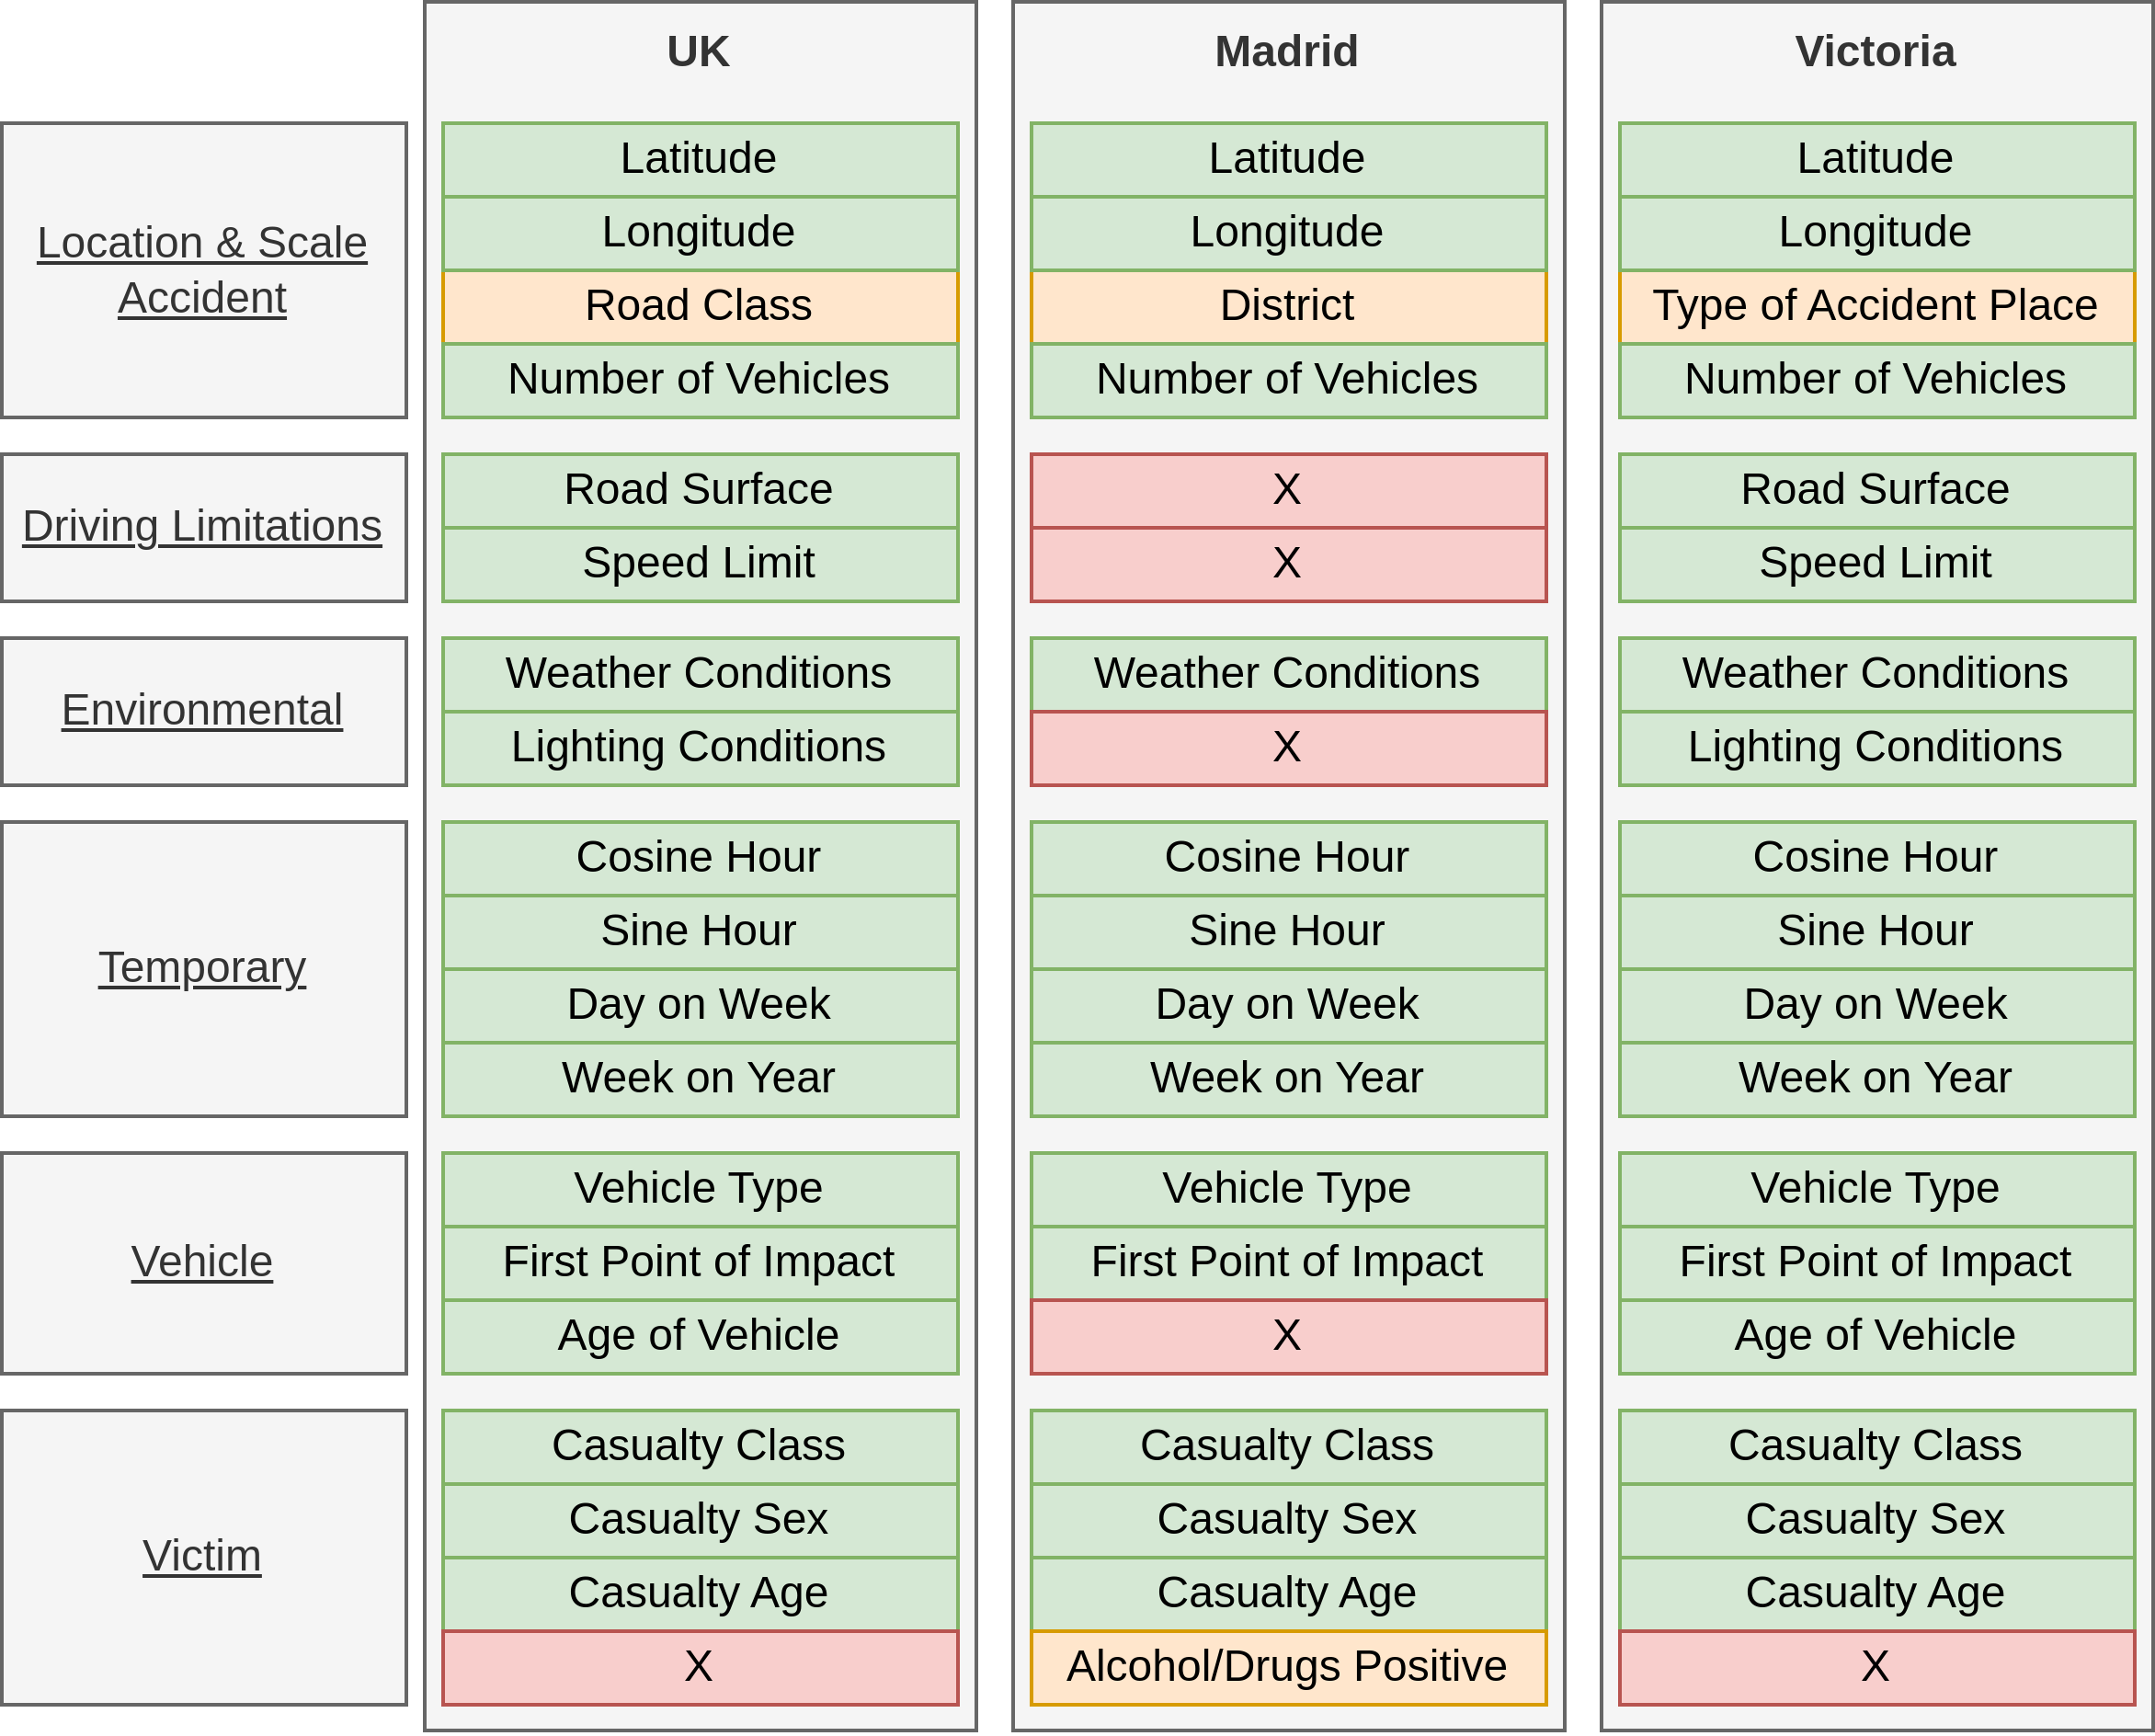
\includegraphics[width=12cm]{Figures/Dataset Comparative.png}
	\caption[Clasificación de variables para el modelo GTAAF]{Clasificación de variables para el modelo GTAAF. Los campos mostrados en amarillo representan características de la misma naturaleza pero difieren en la granularidad de los datos. Además, las características ausentes en comparación con otros conjuntos de datos están resaltadas en rojo}
	\label{FeaturesClassification}
\end{figure}

A continuación se detallarán aquellas partes comunes entre estos tres conjuntos de datos y las principales diferencias entre ellos.

\subsubsection*{Partes comunes entre los datos en base a la categorización}

Normalmente, en cualquier conjunto de datos que describa accidentes, existe información básica y de fácil obtención que suele ser común entre distintas regiones. Estas características suelen presentarse en forma de información espacial y temporal del accidente, como es la localización, las condiciones climáticas en el momento del suceso o la hora y fecha en la que se ha producido, como es el caso entre estos tres conjuntos de datos. Por otra parte, como es lógico, existe información básica que puede ser recogida rápidamente observando la escena del accidente, como es la localización, el número de vehículos implicados, las condiciones climáticas, la hora, el tipo de vehículo, el punto de impacto y las características del accidentado.


\subsubsection*{Principales diferencias entre los datos}

Cada una de las regiones ofrece información distinta en cada conjunto de datos. En este punto se analizarán las principales diferencias entre ellos en base a la categorización propuesta:

\textbf{UK}

En el caso de UK se observan ligeras diferencias respeto al resto de poblaciones. Como es el caso de la característica \textit{Road class} (para la categoría \textit{Localización y Escala del Accidente}), cuyo significado varía en comparación con el resto, y la ausencia de información sobre controles de estupefacientes a la víctima (categoría \textit{Víctima}). En el caso de \textit{Road Class}, este campo representa la clasificación de la carretera en la que se ha producido el accidente en base al tráfico que suele fluctuar sobre ella. Esta clasificación es responsabilidad de Gobierno de Reino Unido y se clasifican las vías en seis tipos diferentes: (1) Motorways: se trata de autopistas de alta velocidad que permiten el movimiento de vehículos entre los principales pueblos y ciudades. (2) A(M): se trata de carreteras principales que interconectan poblaciones y destinos de interés, estas vías pueden contener secciones transformadas en autovía. (3) A: carreteras importantes que conectan grandes densidades de tráfico entre zonas. Generalmente son las más anchas y directas, y son las de mayor importancia para el tráfico que contiene el área, estas carreteras pueden estar abiertas a distintos usuarios, como viandantes, ciclistas o caballos, aunque normalmente esto está restringido por las autoridades locales competentes. (4) Las carreteras B alimentan el tráfico entre las vías A y las carreteras más pequeñas de la red, siguen siendo de especial importancia para el tráfico, pero menos que las A. (5) Las carreteras tipo C son generalmente más pequeñas e interconectan las vías de tipo A y B. Normalmente unen urbanizaciones con el resto de carreteras de la red, son carreteras de menor importancia que las anteriores pero son de mayor relevancia respecto a las del siguiente tipo. (6) Carreteras no clasificadas, se tratan de vías destinadas al tráfico local, por su naturaleza la mayoría de las vías pertenecen a este tipo, generalmente tienen muy poca importancia y a nivel local \cite{UKDepartmentForTransportRoadClassification}.


\textbf{Madrid}

% \textcolor{orange}{\textbf{Luis: estoy llamando a las variables en inglés, pero así están en la tabla comparativa de arriba. Opiniones?}}

En el caso del conjunto de datos de Madrid, las diferencias respecto al resto de regiones se encuentra más acentuada. La información disponible es considerablemente menor en comparación con los datos de Reino Unido y de Victoria. Analizando la Figura \ref{FeaturesClassification} se puede observar que hay ciertas características que no están presentes, llegando a dejar incluso una categoría vacía (\textit{Limitaciones de Conducción}) al no disponer de información de este tipo. Por otra parte, tampoco se dispone de la información de \textit{Lighting Conditions} para la categoría \textit{Ambiental}, ni de \textit{Age of Vehicle}, en la categoría \textit{Vehículo}. No obstante, aún faltando esta información, el resto de características pueden ser asignadas a las categorías definidas, convirtiendo, por tanto, este dataset aplicable a este modelo.

Sin embargo, el conjunto de datos de Madrid ofrece información sobre si la víctima se encuentra bajo los efectos del alcohol o de sustancias estupefacientes. Al ser un dato que describe a la víctima del incidente, este será asignado a la categoría Victim.

Por otro lado, en la categoría \textit{Localización y Escala del Accidente} los datos de Madrid presentan una diferencia en lo que representa la característica \textit{District} respecto al resto de datasets. Este campo contempla el distrito dentro de Madrid en el que se ha producido el accidente, y es interpretado de forma numérica en función del orden de aparición de los distritos en los datos. Al ser una característica que ofrece información sobre la localización del accidente, será incluida en la categoría de \textit{Localización y Escala del Accidente}.

Como diferencia más notable sobre el conjunto de datos de Madrid es que \textbf{dispone de características para contemplar 5 categorías} respecto a las 6 de los otros dos conjuntos de datos.

\textbf{Victoria}

La información disponible en Victoria contempla un caso parecido al de los datos de Reino Unido, donde no se disponen de datos que describan si la víctima se encontraba bajo los efectos de estupefacientes o del alcohol, como es el caso de Madrid. Por lo que esta característica quedará vacía también en este conjunto de datos.

Respecto a la variable \textit{First Point of Impact}, este campo indica el tipo de colisión del vehículo, es decir, contra qué objeto ha impactado el vehículo, en comparación contra otros conjuntos de datos que indican también de qué parte del mismo ha impactado primero.

Por otra parte, la característica \textit{Type Of Accident Place}, ofrece información sobre el lugar del accidente, concretamente el lugar donde se ha producido, como autopista, parking, túnel, etc. por lo que irá asignada a la categoría \textit{Localización y Escala del Accidente}.



\subsection{Limpieza}
En la tabla \ref{DataDistribution} se expone el número total de registros de los datos originales y el número de muestras resultante tras haber aplicado la limpieza de estos datos para cada una de las poblaciones contempladas.

\begin{table}[H]
	\begin{center}
		\caption{Comparación de la distribución de datos tras el proceso de limpieza}
		\begin{tabular}{|c|c||c|c|}
			\hline
			\multicolumn{4}{ |c| }{\textbf{Distribución de Datos}} \\ \hline
			\multicolumn{4}{ |c| }{\textbf{Reino Unido}} \\ \hline
			
			\textbf{Región} & \textbf{Asistencia} & Original & Limpieza
			\\ \hline \hline
			
			\multirow{2}{*}{Southwark} &
			No   & 27.105  & 11.065 \\ &
			Sí  & 3.109   & 2.703 \\ \hline \hline
			\multirow{2}{*}{Manchester} &
			No  & 48.771   & 24.110 \\ &
			Sí  & 4.570    & 1.885 \\ \hline \hline
			\multirow{2}{*}{Birmingham} &
			No  & 108.723  & 64.147 \\ &
			Sí  & 11.187   & 6.191 \\ \hline \hline
			\multirow{2}{*}{Liverpool} &
			No  & 49.291  & 25.936 \\ &
			Sí  & 5.161   & 2.276 \\ \hline \hline
			\multirow{2}{*}{Sheffield} &
			No  & 43.579  & 25.622  \\ &
			Sí  & 5.887   & 2.703  \\ \hline \hline
			\multirow{2}{*}{Cornwall} &
			No  & 32.994 & 20.803 \\ &
			Sí  & 4.852 & 2.842 \\ \hline \hline
			
			\multicolumn{4}{ |c| }{\textbf{España}} \\ \hline
			
			\textbf{Región} & \textbf{Asistencia} & Original & Limpieza
			\\ \hline \hline
			
			\multirow{2}{*}{Madrid} &
			No  & 72.042  & 63.853   \\ &
			Sí & 1.472   & 1.305  \\ \hline \hline
			
			\multicolumn{4}{ |c| }{\textbf{Australia}} \\ \hline
			
			\textbf{Región} & \textbf{Asistencia} & Original & Limpieza
			\\ \hline \hline
			
			\multirow{2}{*}{Victoria} &
			No   & 7.064  & 5.556   \\ &
			Sí  & 7.059  & 6.024 \\ \hline \hline
			
		\end{tabular}

		\label{DataDistribution}
	\end{center}
\end{table}

% UK - Original
% - S: 266884
% - A: 34766
% - T: 301650
% UK - Cleaned
% - S: 197619
% - A: 18600
% - T: 216219
% Madrid
% - O: 60996
% - C: 43554
% Victoria
% - O: 14123
% - C: 11580


Como se puede observar, tras el proceso de limpieza, cada uno de los conjuntos de datos se ve afectado por una pérdida de registros significativa. Para Reino Unido, de un total de $301.650$ registros, se obtienen finalmente $216.219$, lo que supone un $28,3\%$ de pérdida de información respecto a la información inicial. En la ciudad de Madrid, $73,514$ registros en bruto iniciales acaban resultando en $65,158$ con información interpretable, conllevando un $11.38\%$ de pérdida de información. Por último, en el estado de Victoria, de un total de $14.123$ registros iniciales, resultan $11.580$ finales, asumiendo un $18\%$ de pérdida respecto a sus muestras iniciales.

\subsection{Discretización}

En esta sección se expone la discretización escogida para las variables de las tres regiones seleccionados para una mayor comprensión del tratamiento de las características en cada región.

\subsubsection*{Reino Unido}

La tabla \ref{UKFeaturesClassification} muestra la asignación de valores numéricos aplicada a los datos de las regiones de Reino Unido (Southwark, Manchester, Birmingham, Liverpool, Sheffield y Cornwall).

%%%%%%%%%%%%%%%%%%%%%%%%%%%%%%%%%%%%%%%%%%%%%%%%%%%%%%%%%%%%%%%%%%%%%%%%%%%%%%%%%
\begin{table}[H]
	\caption{Discretización propuesta de las variables para el conjunto de datos de Reino Unido}
	\scriptsize
	\begin{center}
		\begin{tabular}{|c|c|c|c|}
			\hline
			\textbf{Categoría} & \textbf{Característica} & \textbf{Valor} & \textbf{Descripción} \\ \hline 
			\hline
			
			\multirow{9}{*}{\textbf{\makecell{Localización y \\ Escala del accidente}}}
			& Latitud  & Número Real & Coordenada Este (OSGR) \\ \cline{2-4}
			& Longitud & Número Real & Coordenada Norte (OSGR) \\ \cline{2-4}
			& \multirow{6}{*} {Clase de Carretera}
			& 0 & Autopista \\ \cline{3-4}
			&& 1 & A(M) \\ \cline{3-4}
			&& 2 & A \\ \cline{3-4}
			&& 3 & B \\ \cline{3-4}
			&& 4 & C \\ \cline{3-4}
			&& 5 & No clasificada \\ \cline{2-4}
			& Número de Vehículos & 0-N & Dependiendo de los vehículos involucrados \\ \cline{2-4}
			
			\hline
			\hline
			
			\multirow{6}{*}{\textbf{\makecell{Limitaciones \\ de Conducción}}}
			& \multirow{5}{*} {Superficie de la Carretera}
			& 0 & Seca \\ \cline{3-4}
			&& 1 & Mojada / Húmeda \\ \cline{3-4}
			&& 2 & Nieve \\ \cline{3-4}
			&& 3 & Helada / Hielo \\ \cline{3-4}
			&& 4 & Inundación  \\ \cline{2-4}
			& Límite de Velocidad & 0-70 & Dependiendo del límite de velocidad (mph) \\ \cline{2-4}
			
			\hline
			\hline
			
			\multirow{13}{*}{\textbf{\makecell{Factores Ambientales}}} 
			& \multirow{8}{*} {Condiciones Meteorológicas}
			& 0 & Buen tiempo sin viento fuerte \\ \cline{3-4}
			&& 1 & Lluvia sin viento fuerte \\ \cline{3-4}
			&& 2 & Nieve sin viento fuerte \\ \cline{3-4}
			&& 3 & Buen tiempo con viento fuerte \\ \cline{3-4}
			&& 4 & Lluvia con viento fuerte \\ \cline{3-4}
			&& 5 & Nieve con viento fuerte \\ \cline{3-4}
			&& 6 & Niebla o neblina \\ \cline{3-4}
			&& 7 & Otro  \\ \cline{2-4}
			
			& \multirow{5}{*} {Condiciones de Iluminación}
			& 0 & Luz del día: luces de la calle presentes \\ \cline{3-4}
			&& 1 & Oscuridad: sin iluminación en la calle \\ \cline{3-4}
			&& 2 & Oscuridad: luces de la calle encendidas \\ \cline{3-4}
			&& 3 & Oscuridad: luces de la calle apagadas \\ \cline{3-4}
			&& 4 & Oscuridad: iluminación desconocida  \\ \cline{2-4}
			
			\hline
			\hline
			
			\multirow{4}{*}{\textbf{\makecell{Temporal}}} 
			& Hora Coseno & Número Real & Representación cosenoidal de la hora \\ \cline{2-4}
			& Hora Seno & Número Real & Representación senoidal de la hora \\ \cline{2-4}
			& Día de la Semana & 0-6 & Dependiendo del día de la semana \\ \cline{2-4}
			& Semana del Año & 0-52 & Dependiendo de la semana \\ \cline{2-4}
			
			\hline
			\hline
			
			\multirow{7}{*}{\textbf{Vehículo}}
			& Tipo de Vehículo & 0-17 & Dependiendo del peso del vehículo \\ \cline{2-4}
			& \multirow{5}{*} {Primer Punto de Impacto}
			& 0 & No impactó \\ \cline{3-4}
			&& 1 & Frente \\ \cline{3-4}
			&& 2 & Parte trasera \\ \cline{3-4}
			&& 3 & Lado contrario \\ \cline{3-4}
			&& 4 & Lado cercano \\ \cline{3-4}
			&& 5 & Desconocido (autoreportado) \\ \cline{2-4}
			& Edad del Vehículo  & 0-N & En orden de antigüedad del vehículo \\ \cline{2-4}
			
			\hline
			\hline
			
			\multirow{9}{*}{\textbf{Víctima}}
			& \multirow{3}{*} {Clase de Víctima}
			& 0 & Conductor/Motociclista \\ \cline{3-4}
			&& 1 & Pasajero \\ \cline{3-4}
			&& 2 & Peatón  \\ \cline{2-4}
			& \multirow{2}{*} {Sexo de la Víctima}
			& 0 & Masculino \\ \cline{3-4}
			&& 1 & Femenino  \\ \cline{2-4}
			& \multirow{4}{*} {Edad de la Víctima}
			& 0 & Menor de 18 años \\ \cline{3-4}
			&& 1 & Entre 18 y 25 años \\ \cline{3-4}
			&& 2 & Entre 25 y 65 años \\ \cline{3-4}
			&& 3 & Mayor de 65 años  \\ \cline{2-4}
			
			\hline
			\hline
		\end{tabular}
	\end{center}

	\label{UKFeaturesClassification}
\end{table}

%%%%%%%%%%%%%%%%%%%%%%%%%%%%%%%%%%%%%%%%%%%%%%%%%%%%%%%%%%%%%%%%%%%%%%%%%%%%%%%%%

\subsubsection*{Madrid}

La tabla \ref{MadridFeaturesClassification} muestra la asignación de valores aplicada a los datos de la región de Madrid. Como cuestión a considerar en este caso es que a la variable Distrito se le aplica un valor numérico en funcón del orden de aparición, sin que este represente ninguna importancia incremental.

%%%%%%%%%%%%%%%%%%%%%%%%%%%%%%%%%%%%%%%%%%%%%%%%%%%%%%%%%%%%%%%%%%%%%%%%%%%%%%%%%
\begin{table}[H]
	\caption{Discretización propuesta de las variables para el conjunto de datos de Madrid}
	\scriptsize
	\centering
	\begin{center}
		\begin{tabular}{|c|c|c|c|}
			\hline
			\textbf{Categoría} & \textbf{Característica} & \textbf{Valor} & \textbf{Descripción} \\ \hline 
			\hline
			
			\multirow{4}{*}{\textbf{\makecell{Localización \& \\ Escala del Accidente}}}
			& Latitud  & Número Real & Sistema de coordenadas cartesianas \\ \cline{2-4}
			& Longitud & Número Real & Sistema de coordenadas cartesianas \\ \cline{2-4}
			& Distrito  & 0-X & Número de distrito \\ \cline{2-4}
			& Número de Vehículos & 0-N & Dependiendo de los vehículos involucrados \\ \cline{2-4}
			\hline
			\hline
			
			\multirow{7}{*}{\textbf{\makecell{Factores Ambientales}}} 
			& \multirow{8}{*} {Condiciones Meteorológicas}
			& 0 & Despejado \\ \cline{3-4}
			&& 1 & Nublado \\ \cline{3-4}
			&& 2 & Lluvia ligera \\ \cline{3-4}
			&& 3 & Lluvia intensa \\ \cline{3-4}
			&& 4 & Granizo \\ \cline{3-4}
			&& 5 & Nevando \\ \cline{3-4}
			&& 6 & Desconocido \\ \cline{2-4}
			
			
			\hline
			\hline
			
			\multirow{4}{*}{\textbf{\makecell{Temporal}}} 
			& Hora Coseno & Número Real & Representación cosenoidal de la hora \\ \cline{2-4}
			& Hora Seno & Número Real & Representación senosoidal de la hora\\ \cline{2-4}
			& Día de la Semana & 0-6 & Dependiendo del día de la semana\\ \cline{2-4}
			& Semana del Año & 0-52 & Dependiendo de la semana \\ \cline{2-4}
			
			\hline
			\hline
			
			\multirow{15}{*}{\textbf{Vehículo}}
			& Tipo de Vehículo & 0-17 & Dependiendo del peso del vehículo \\ \cline{2-4}
			& \multirow{12}{*} {Primer Punto de Impacto}
			&  0 &  Colisión frontal - tamaño \\ \cline{3-4}
			&& 1 &  Colisión trasera \\ \cline{3-4}
			&& 2 &  Choque lateral \\ \cline{3-4}
			&& 3 &  Colisión contra obstáculo fijo \\ \cline{3-4}
			&& 4 &  Choque en cadena \\ \cline{3-4}
			&& 5 &  Atropello a peatón \\ \cline{3-4}
			&& 6 &  Colisión frontal \\ \cline{3-4}
			&& 7 &  Otro \\ \cline{3-4}
			&& 8 &  Abandonando la carretera \\ \cline{3-4}
			&& 9 &  Vuelco del vehículo \\ \cline{3-4}
			&& 10 &  Atropello a animal \\ \cline{3-4}
			&& 11 &  Caída \\ \cline{3-4}
			\hline
			\hline
			
			\multirow{9}{*}{\textbf{Víctima}}
			& \multirow{3}{*} {Clase de Víctima}
			& 0 & Conductor/Motociclista \\ \cline{3-4}
			&& 1 & Pasajero \\ \cline{3-4}
			&& 2 & Peatón  \\ \cline{2-4}
			& \multirow{2}{*} {Sexo de la Víctima}
			& 0 & Masculino \\ \cline{3-4}
			&& 1 & Femenino  \\ \cline{2-4}
			& \multirow{4}{*} {Edad de la Víctima}
			& 0 & Menor de 18 años \\ \cline{3-4}
			&& 1 & Entre 18 y 25 años \\ \cline{3-4}
			&& 2 & Entre 25 y 65 años \\ \cline{3-4}
			&& 3 & Mayor de 65 años  \\ \cline{2-4}
			& \multirow{2}{*} {Alcohol/Drogas Positivo}
			& 0 & No \\ \cline{3-4}
			&& 1 & Sí \\ \cline{3-4}
			\hline
			\hline
		\end{tabular}
	\end{center}

	\label{MadridFeaturesClassification}
\end{table}
%%%%%%%%%%%%%%%%%%%%%%%%%%%%%%%%%%%%%%%%%%%%%%%%%%%%%%%%%%%%%%%%%%%%%%%%%%%%%%%%%

\subsubsection*{Victoria}

La tabla \ref{VictoriaFeaturesClassification} muestra la discretización del valor las características que pueden tomar los registros de accidentes en el Estado de Victoria.

%%%%%%%%%%%%%%%%%%%%%%%%%%%%%%%%%%%%%%%%%%%%%%%%%%%%%%%%%%%%%%%%%%%%%%%%%%%%%%%%%
\begin{table}[H]
	\caption{Discretización propuesta de las variables para el conjunto de datos de Victoria}
	\scriptsize
	\begin{center}
		\begin{tabular}{|c|c|c|c|}
			\hline
			\textbf{Categoría} & \textbf{Característica} & \textbf{Valor} & \textbf{Descripción} \\ \hline 
			\hline
			
			\multirow{4}{*}{\textbf{\makecell{Localización \& \\ Escala del Accidente}}}
			& Latitud  & Número Real & Coordenada Este OSGR \\ \cline{2-4}
			& Longitud & Número Real & Coordenada Norte OSGR \\ \cline{2-4}
			& Clase de Carretera & 0-58 & En orden de aparición \\ \cline{2-4}
			& Número de Vehículos & 0-N & Dependiendo de los vehículos involucrados \\ \cline{2-4}
			
			\hline
			\hline
			
			
			\multirow{7}{*}{\textbf{\makecell{Limitaciones \\ de Conducción}}}
			& \multirow{6}{*} {Superficie de la Carretera}
			& 0 & Seco \\ \cline{3-4}
			&& 1 & Mojado / Húmedo \\ \cline{3-4}
			&& 2 & Fangosa \\ \cline{3-4}
			&& 3 & Nevada \\ \cline{3-4}
			&& 4 & Hielo  \\ \cline{3-4}
			&& 5 & Otro  \\ \cline{2-4}
			& Límite de Velocidad & 0-70 & Dependiendo del límite de velocidad (mph) \\ \cline{2-4}
			
			\hline
			\hline
			
			\multirow{15}{*}{\textbf{\makecell{Factores Ambientales}}} 
			& \multirow{8}{*} {Condiciones Meteorológicas}
			& 0 & Despejado \\ \cline{3-4}
			&& 1 & Lluvia \\ \cline{3-4}
			&& 2 & Nevando \\ \cline{3-4}
			&& 3 & Niebla \\ \cline{3-4}
			&& 4 & Humo en el ambiente \\ \cline{3-4}
			&& 5 & Polvo en el ambiente \\ \cline{3-4}
			&& 6 & Fuertes Vientos \\ \cline{3-4}
			&& 7 & Otro  \\ \cline{2-4}
			
			& \multirow{7}{*} {Condiciones de Iluminación}
			& 0 & Día \\ \cline{3-4}
			&& 1 & Amanecer \\ \cline{3-4}
			&& 2 & Oscuridad: luces de la calle encendidas \\ \cline{3-4}
			&& 3 & Oscuridad: luces de la calle apagadas \\ \cline{3-4}
			&& 4 & Oscuridad: sin luces de la calle \\ \cline{3-4}
			&& 5 & Oscuridad: iluminación desconocida \\ \cline{3-4}
			&& 6 & Otro  \\ \cline{2-4}
			
			\hline
			\hline
			
			\multirow{4}{*}{\textbf{\makecell{Temporal}}} 
			& Hora Coseno & Número Real & Representación cosenoidal de la hora\\ \cline{2-4}
			& Hora Seno & Número Real & Representación senosoidal de la hora\\ \cline{2-4}
			& Día de la Semana & 0-6 & Dependiendo del día de la semana \\ \cline{2-4}
			& Semana del Año & 0-52 & Dependiendo de la semana \\ \cline{2-4}
			
			\hline
			\hline
			
			\multirow{10}{*}{\textbf{Vehículo}}
			& Tipo de Vehículo & 0-17 & Dependiendo del peso del vehículo \\ \cline{2-4}
			& \multirow{8}{*} {Primer Punto de Impacto}
			& 0 & Colisión con vehículo \\ \cline{3-4}
			&& 1 & Atropello a peatón \\ \cline{3-4}
			&& 2 & Atropello a animal \\ \cline{3-4}
			&& 3 & Colisión contra obstáculo fijo \\ \cline{3-4}
			&& 3 & Colisión contra otro objeto \\ \cline{3-4}
			&& 5 & Vuelco del vehículo (sin colisión) \\ \cline{3-4}
			&& 6 & Caída desde vehículo en movimiento \\ \cline{3-4}
			&& 7 & Sin colisión y sin objeto golpeado) \\ \cline{2-4}
			& Edad del Vehículo  & 0-N & En orden de antigüedad del vehículo \\ \cline{2-4}
			
			\hline
			\hline
			
			\multirow{12}{*}{\textbf{Víctima}}
			& \multirow{6}{*} {Clase de Víctima}
			& 0 & Peatón \\ \cline{3-4}
			&& 1 & Conductor \\ \cline{3-4}
			&& 2 & Pasajero \\ \cline{3-4}
			&& 3 & Motociclista \\ \cline{3-4}
			&& 4 & Ciclista \\ \cline{3-4}
			&& 5 & Desconocido  \\ \cline{2-4}
			& \multirow{2}{*} {Sexo de la Víctima}
			& 0 & Masculino \\ \cline{3-4}
			&& 1 & Femenino  \\ \cline{2-4}
			& \multirow{4}{*} {Edad de la Víctima}
			& 0 & Menor de 18 años \\ \cline{3-4}
			&& 1 & Entre 18 y 25 años \\ \cline{3-4}
			&& 2 & Entre 25 y 65 años \\ \cline{3-4}
			&& 3 & Mayor de 65 años  \\ \cline{2-4}
			
			\hline
			\hline
		\end{tabular}
	\end{center}

	\label{VictoriaFeaturesClassification}
\end{table}
%%%%%%%%%%%%%%%%%%%%%%%%%%%%%%%%%%%%%%%%%%%%%%%%%%%%%%%%%%%%%%%%%%%%%%%%%%%%%%%%%


\subsection{Filtrado de áreas}


Para ilustrar los parámetros con los que se aplica el filtrado de áreas, se presenta la Tabla \ref{AreasInformation}, donde se muestra para cada población el número de áreas proyectadas resultante de la elección del tamaño de las ventanas en función de los valores \textit{X,Y}. La elección de estos tamaños variará función de la extensión y densidad de población, tomando valores de ventana más grandes en poblaciones más dispersas y tamaños más pequeños cuando la densidad de población es más alta. Los tamaños de ventana para cada población han sido escogidos mediante un procedimiento experimental, en el que se maximiza el rendimiento final de los modelos en base a la media total.

\begin{table}[H]
	\caption{Número de áreas resultante tras la definición de su tamaño para cada región}
	\begin{center}
		\begin{tabular}{|c|c||c|c|c||c|c|c}
			\hline
			\multicolumn{4}{ |c| }{\textbf{División de Áreas}} \\ \hline
			
			\multicolumn{4}{ |c| }{\textbf{Reino Unido}} \\ \hline
			\textbf{Región} & \textbf{Eje} & \textbf{Número de Áreas} & \textbf{Tamaño de Área}
			\\ \hline  \hline 
			
			\multirow{2}{*}{Southwark} &
			X  & 529  & 10 \\ &
			Y  & 487  & 20 \\ \hline \hline
			\multirow{2}{*}{Manchester} &
			X  & 791     & 14  \\ &
			Y  & 1.069    & 20  \\ \hline \hline
			\multirow{2}{*}{Birmingham} &
			X  & 3.519    & 12 \\ &
			Y  & 1.557    & 17 \\ \hline \hline
			\multirow{2}{*}{Liverpool} &
			X  & 2.107    & 12  \\ &
			Y  & 717     & 21  \\ \hline \hline
			\multirow{2}{*}{Sheffield} &
			X  & 1.896     & 12  \\ &
			Y  & 1.115     & 18 \\ \hline \hline
			\multirow{2}{*}{Cornwall} &
			X  & 10.090    & 15 \\ &
			Y  & 5.597    & 19 \\ \hline \hline
			
			\multicolumn{4}{ |c| }{\textbf{España}} \\ \hline
			\textbf{Región} & \textbf{Eje} & \textbf{Número de Áreas} & \textbf{Tamaño de Área}
			\\ \hline  \hline 
			
			\multirow{2}{*}{Madrid} &
			X  & 5.241  & 5 \\ &
			Y  & 4.444  & 7 \\ \hline \hline
			
			\multicolumn{4}{ |c| }{\textbf{Australia}} \\ \hline
			\textbf{Región} & \textbf{Eje} & \textbf{Número de Áreas} & \textbf{Tamaño de Área}
			\\ \hline  \hline 
			
			\multirow{2}{*}{Victoria} &
			X  & 4.931  & 145 \\ &
			Y  & 5.241  & 97 \\ \hline \hline
		\end{tabular}
	\end{center}

	\label{AreasInformation}
\end{table}

Una vez se establecen las dimensiones de las ventanas de tamaño $X,Y$ se aplica el filtrado para cada región, donde el número de muestras de la clase mayoritaria se ve considerablemente reducido respecto a la minoritaria, buscando obtener un conjunto de datos más balanceado. La Tabla \ref{DataDistributionFiltered} muestra el número de registros originales para cada población y el número de registros resultante tras aplicar el filtrado.

%%%%%%%%%%%%%%%%%%%%%%%%%%%%%%%%%%%%%%%%%%%%%%%%%%%%%%%%%%%%%%%%%%%%%%%%%%%%%%%%%
\begin{table}[H]
	\caption{Distribución de datos tras el proceso de filtrado para cada una de las regiones}
	\begin{center}
		\begin{tabular}{|c|c||c|c|}
			\hline
			\multicolumn{4}{ |c| }{\textbf{Distribución de Datos}} \\ \hline
			\multicolumn{4}{ |c| }{\textbf{Reino Unido}} \\ \hline
			
			\textbf{Región} & \textbf{Asistencia} & Limpieza & Filtrado
			\\ \hline \hline
			
			\multirow{2}{*}{Southwark} &
			No   & 11.065  & 4.251 \\ &
			Sí  & 2.703   & 1.256 \\ \hline \hline
			\multirow{2}{*}{Manchester} &
			No  & 24.110  & 4.548 \\ &
			Sí & 1.885   & 1.466 \\ \hline \hline
			\multirow{2}{*}{Birmingham} &
			No  & 64.147  & 4.092 \\ &
			Sí & 6.191   & 2.063 \\ \hline \hline
			\multirow{2}{*}{Liverpool} &
			No  & 25.936  & 3.640 \\ &
			Sí & 2.276   & 1.192 \\ \hline \hline
			\multirow{2}{*}{Sheffield} &
			No  & 25.622 & 2.060  \\ &
			Sí & 2.703  & 1.638  \\ \hline \hline
			\multirow{2}{*}{Cornwall} &
			No  & 20.803 & 2.191 \\ &
			Sí & 2.842  & 2.020 \\ \hline \hline
			
			\multicolumn{4}{ |c| }{\textbf{España}} \\ \hline
			
			\textbf{Región} & \textbf{Asistencia} & Limpieza & Filtrado
			\\ \hline \hline
			
			\multirow{2}{*}{Madrid} &
			No   & 63.840  & 2.601 \\ &
			Sí  & 1.305   & 1.286 \\ \hline \hline
			
			\multicolumn{4}{ |c| }{\textbf{Australia}} \\ \hline
			
			\textbf{Región} & \textbf{Asistencia} & Limpieza & Filtrado
			\\ \hline \hline
			
			\multirow{2}{*}{Victoria} &
			No   & 5.556  & 2.065  \\ &
			Sí  & 6.024  & 2.649  \\ \hline \hline
			
		\end{tabular}
	\end{center}

	\label{DataDistributionFiltered}
\end{table}

% UK
%     Original
%     - S: 171683
%     - A: 18600
% UK
%     Filtered
%     - S: 20782
%     - A: 9635
% Madrid
%     Cleaned: 43554
%     Filtered: 3887
% Victoria
%     Cleaned: 11580
%     Filtered: 4714

Una vez aplicado el filtrado de áreas los conjuntos de datos resultantes presentan un desbalanceo considerablemente menor. Para el dataset de Reino Unido se ha conseguido reducir, de media, una desproporción de las clases del $90,2\%$ y $9,8\%$ de los registros de las clases Sin Asistencia y Con Asistencia respectivamente hasta un  $53,6\%$ y $46,4\%$. Para la ciudad de Madrid se partía con un $98\%$ de accidentes Sin Asistencia y un $2\%$ de accidentes Con Asistencia, llegando una proporción final del  $67\%$ y $33\%$ respectivamente. Para la ciudad de Victoria se evoluciona desde un $48\%$ y $52\%$ a un $43,8\%$ $56,2\%$, por lo que sobre esta última, el proceso de remuestreo de clases afectará a la clase Sin Asistencia, siendo el único caso en el que esta es mayoritaria.

\subsection{Resampling}

En esta fase se seleccionan los datos de entrenamiento y de test. La distribución de esta división presenta un 80\% de los datos refinados como conjunto de entrenamiento, y 20\% restante como conjunto de validación o test. En la tabla \ref{Resampling} se muestra la distribución de estos datos junto con el número total de muestras de entrenamiento sobre el que se ha aplicado el proceso de aumentado de datos \textit{SMOTE-II}.

En la tabla \ref{Resampling} se muestran los datos resultantes tras haber aplicado el proceso de resampling mediante la generación de datos sintéticos de \textit{SMOTE-II}, conformando un dataset balanceado en el que se previene el riesgo de sesgo de datos por parte de los modelos.

%%%%%%%%%%%%%%%%%%%%%%%%%%%%%%%%%%%%%%%%%%%%%%%%%%%%%%%%%%%%%%%%%%%%%%%%%%%%%%%%%
\begin{table}[H]
	\caption[Distribución de datos para las ciudades seleccionadas. Modelo GTAAF]{Distribución de datos para las ciudades seleccionadas. Modelo GTAAF. La columna Asistencia representa si el accidente ha requerido de asistencia o no, las dos clases objetivo de este documento. La columna Filtrado indica el número de muestras disponibles tras el proceso de filtrado. La columna Entrenamiento representa el 80\% de las muestras de entrenamiento seleccionadas del total de los datos filtrados. La columna Test muestra el 20\% de los datos utilizados para la futura validación de los modelos. Finalmente \textit{Oversampled} engloba el número de muestra tras aplicar el aumentado de datos sobre el conjunto de entrenamiento de cada población mediante la técnica \textit{SMOTE-II} para la clase minoritaria}
	\begin{center}
		\begin{tabular}{|c|c||c|c|c|c|}
			\hline
			\multicolumn{6}{ |c| }{\textbf{Distribución de Datos}} \\ \hline
			\multicolumn{6}{ |c| }{\textbf{Reino Unido}} \\ \hline
			
			\textbf{Región} & \textbf{Asistencia} & Filtrado & Entrenamiento & Test & \textit{Oversampled}
			\\ \hline \hline
			
			\multirow{2}{*}{Southwark} &
			No   & 4.251  & 3.400 & 851 & 3.400  \\ &
			Sí  & 1.256  & 1.004 & 252 & 3.400 \\ \hline \hline
			\multirow{2}{*}{Manchester} &
			No   & 4.548  & 3.638 & 910 & 3.638 \\ &
			Sí  & 1.466  & 1.172 & 294 & 3.638 \\ \hline \hline
			\multirow{2}{*}{Birmingham} &
			No   & 4.092  & 3.273 & 819 & 3.273 \\ &
			Sí  & 2.063  & 1.650 & 413 & 3.273 \\ \hline \hline
			\multirow{2}{*}{Liverpool} &
			No   & 3.640 & 2.912 & 728 & 2.912  \\ &
			Sí  & 1.192 &   953 & 239 & 2.912 \\ \hline \hline
			\multirow{2}{*}{Sheffield} &
			No   & 2.060  & 1.648 & 412 & 1.648 \\ &
			Sí  & 1.638  & 1.310 & 328 & 1.648 \\ \hline \hline
			\multirow{2}{*}{Cornwall} &
			No   & 2.191  & 1.752 & 439 & 1.752 \\ &
			Sí  & 2.020  & 1.616 & 404 & 1.752 \\ \hline \hline
			
			\multicolumn{6}{ |c| }{\textbf{España}} \\ \hline
			\textbf{Región} & \textbf{Asistencia} & Filtrado & Entrenamiento & Test & \textit{Oversampled}
			\\ \hline \hline
			
			\multirow{2}{*}{Madrid} &
			No   & 2.601  & 2.080 & 521 & 2.080  \\ &
			Sí  & 1.286  & 1.028 & 258 & 2.080 \\ \hline \hline
			
			\multicolumn{6}{ |c| }{\textbf{Australia}} \\ \hline
			\textbf{Región} & \textbf{Asistencia} & Filtrado & Entrenamiento & Test & \textit{Oversampled}
			\\ \hline \hline
			
			\multirow{2}{*}{Victoria} &
			No   & 2.065 & 1.652 & 413 & 2.119  \\ &
			Sí  & 2.649 & 2.119 & 530 & 2.119 \\ \hline \hline
		\end{tabular}
	\end{center}

	\label{Resampling}
\end{table}
%%%%%%%%%%%%%%%%%%%%%%%%%%%%%%%%%%%%%%%%%%%%%%%%%%%%%%%%%%%%%%%%%%%%%%%%%%%%%%%%%


\subsection{Normalización}


En la Tabla \ref{FeaturesNormalizationExample} se muestra un ejemplo de la aplicación de la normalización de datos en base a la técnica \textit{Z-Score}, donde en la primera columna se observan los datos discretizados, mientras que la segunda columna contiene los valores de estas características normalizados.

\begin{table}[H]
	\caption{Ejemplo de muestra original y muestra normalizada}
	\begin{center}
		\begin{tabular}{|c|c||c|c|}
			\hline
			
			\textbf{Categoría} & \textbf{Característica} & \textbf{Valor Discretizado} & \textbf{Valor Normalizado}
			\\ \hline \hline
			
			\multirow{4}{*}{\textbf{\makecell{Location \& \\ Scale Accident}}} &
			Easting & 2511861.414 & -0.527831\\
			& Northing & 2374246.840 &  -1.057103\\
			& 1st Road Class & 3 &  -0.167530\\
			& Number of Vehicles & 2 &  -0.322890\\ \hline \hline
			\multirow{2}{*}{\textbf{\makecell{Driving \\ Limitations}}} &
			Road Surface & 1 & -0.265693 \\
			& Speed Limit & 80 &  -0.005659 \\ \hline \hline
			\multirow{2}{*}{\textbf{Environmental}} &
			Weather Conditions & 1 & -0.259213 \\
			& Lighting Conditions & 1 &  -0.479225\\ \hline \hline
			\multirow{4}{*}{\textbf{Temporary}} &
			Cosine Hour & -0.9659258 & -1.055298 \\
			& Sine Hour & 0.258819 &  0.840276 \\
			& Day on Week & 4 &  -0.055442 \\
			& Week on Year & 52 &  0.844870 \\ \hline \hline
			\multirow{3}{*}{\textbf{Vehicle}} &
			Vehicle Type & 1 & -0.294511 \\
			& First Point of Impact & 1 &  -0.363744 \\
			& Age of Vehicle & 1992 &  -0.062428 \\ \hline \hline
			\multirow{3}{*}{\textbf{Victim}} &
			Casualty Class & 3 & 0.724902 \\
			& Casualty Sex & 0 &  -0.858795 \\
			& Casualty Age & 1 &  -2.062940 \\ \hline \hline
		\end{tabular}
	\end{center}

	\label{FeaturesNormalizationExample}
\end{table}



Una vez se disponen de los datos normalizados, estos ya son comparables y por tanto pueden ser utilizados para el entrenamiento de cualquier modelo que acepte valores numéricos como entrada.


\subsection{Algoritmo Genético}


En la tabla \ref{GAHyperparametersSetup} se muestran los hiperparámetros del algoritmo genético utilizados para optimizar el algoritmo \textit{XGBoost}. Durante cada una de las generaciones, el límite máximo en la población es de 50 individuos (fila \textit{Población}). Estos individuos en cada generación son evaluados mediante la función heurística a optimizar, la métrica \textit{F1-Score} resultante del algoritmo \textit{XGBoost}, entrenado con dicha configuración de hiperparámetros, sobre el conjunto de test accidentes, es decir, en los accidentes no vistos durante el entrenamiento (fila \textit{Función Heurística}). Una vez son evaluados, aquellos 10 mejores individuos son seleccionados para intercambiar su información, los padres que darán lugar a 10 nuevos individuos de cara a la próxima generación (fila \textit{Padres Emparejados}). La mezcla de información entre padres se realiza mediante una estrategia de cruce mixta (fila \textit{Índice de Cruzamiento}), es decir, para cada par de padres se asigna un índice aleatorio en sobre el que se dividirán ambos individuos para luego combinar esta información en el descendiente resultante mediante cruce por punto aleatorio de las soluciones. Una vez se han dado lugar a los 10 nuevos individuos, el valor de cada una de las componentes que los conforman pueden ser modificados con una probabilidad del 40\% (fila \textit{Probabilidad de Mutación)}. Este proceso será repetido a lo largo de todas las 50 generaciones (fila \textit{Generaciones}).


%%%%%%%%%%%%%%%%%%%%%%%%%%%%%%%%%%%%%%%%%%%%%%%%%%%%%%%%%%%%%%%%%%%%%%%%%%%%%%%%%
\begin{table}[H]
	\caption{Configuración de hiperparámetros del algoritmo genético para el modelo GTAAF}
	\centering
	\begin{tabular}{|c|c|}
		\hline
		\textbf{Hiperparámetro} & \textbf{Valor} \\ \hline
		\hline
		Población     & 50 \\ \hline
		Padres Emparejados & 10 \\ \hline
		Generaciones    & 50 \\ \hline
		Índice de Cruzamiento & Aleatorio \\ \hline
		Probabilidad de Mutación & 0.4 \\ \hline
		Función Heurística & Puntuación \textit{F1-Score} del \textit{XGBoost} \\ \hline \hline
	\end{tabular}

	\label{GAHyperparametersSetup}
\end{table}
%%%%%%%%%%%%%%%%%%%%%%%%%%%%%%%%%%%%%%%%%%%%%%%%%%%%%%%%%%%%%%%%%%%%%%%%%%%%%%%%%

La Tabla \ref{MutationXGBoostParams} muestra las variaciones en los valores máximos y mínimos permitidos para cada variable a optimizar mediante el algoritmo genético. La fila \textit{Inicial} de cada hiperparámetro muestra el rango de valores que cada individuo puede tomar cuando es inicializado. En la fila \textit{Mutación} se observan, para cada hiperparámetro, los valores límites permitidos sobre los que los componentes de un sujeto pueden modificarse en el proceso de mutación, siempre y cuando dicho componente haya sido seleccionado para mutarse.

%%%%%%%%%%%%%%%%%%%%%%%%%%%%%%%%%%%%%%%%%%%%%%%%%%%%%%%%%%%%%%%%%%%%%%%%%%%%%%%%%
\begin{table}[H]
	\caption{Límites de inicialización y mutación de los hiperparámetros del algoritmo genético del modelo GTAAF}
	\begin{center}
		\begin{tabular}{|c|c||c|c|}
			\hline
			\textbf{Hiperparámetro} & \textbf{Límite} & \textbf{Mínimo} & \textbf{Máximo}
			\\ \hline \hline
			
			\multirow{2}{*}{ETA} &
			Inicial  & 0.01  & 1  \\ &
			Mutación & -0.2  & 0.2 \\ \hline \hline
			\multirow{2}{*}{Profundidad Máxima} &
			Inicial  & 1   & 25  \\ &
			Mutación & -3  & 3 \\ \hline \hline
			\multirow{2}{*}{Peso Mínimo de Hijos} &
			Inicial  & 0.01   & 20  \\ &
			Mutación & -4  & 4 \\ \hline \hline
		\end{tabular}
	\end{center}

	\label{MutationXGBoostParams}
\end{table}
%%%%%%%%%%%%%%%%%%%%%%%%%%%%%%%%%%%%%%%%%%%%%%%%%%%%%%%%%%%%%%%%%%%%%%%%%%%%%%%%%

La configuración de estos parámetros, tanto los iniciales como los de mutación, se han escogido en base a resultados experimentales, donde se ha priorizado la maximización de la métrica \textit{F1-Score} entre distintos experimentos.

En la Tabla \ref{ResultingHyperparamsXGBoost} se pueden observar los hiperparámetros óptimos resultantes de la ejecución del algoritmo genético, donde para cada región se observa la tasa de aprendizaje de los árboles (\textit{ETA}), la profundidad máxima de los árboles y el peso mínimo de los hijos para decidir la separación a través del nivel de los árboles.

%%%%%%%%%%%%%%%%%%%%%%%%%%%%%%%%%%%%%%%%%%%%%%%%%%%%%%%%%%%%%%%%%%%%%%%%%%%%%%%%%
\begin{table}[H]
	\caption{Hiperparámetros resultantes del \textit{XGBoost} después de ejecutar el algoritmo genético del modelo GTAAF}
	\begin{center}
		\begin{tabular}{|c||c|c|c|}
			\hline
			\multicolumn{4}{ |c| }{\textbf{Valores Resultantes del Algoritmo Genético}} \\ \hline
			
			\multicolumn{4}{ |c| }{\textbf{Reino Unido}} \\ \hline
			
			\textbf{Región} & \textbf{ETA} & \textbf{Profundidad Máxima} & \textbf{Peso Mínimo de Hijos}
			\\ \hline \hline
			
			\multirow{1}{*}{Southwark} &
			0.62  & 13 & 0.01 \\ \hline
			\multirow{1}{*}{Manchester} &
			0.01  & 1  & 0.01  \\ \hline
			\multirow{1}{*}{Birmingham} &
			0.43  & 17  & 0.01 \\ \hline
			\multirow{1}{*}{Liverpool} &
			0.83  & 12  & 0.01  \\ \hline
			\multirow{1}{*}{Sheffield} &
			0.59  & 20  & 0.61 \\ \hline
			\multirow{1}{*}{Cornwall} &
			0.85  & 17 & 0.01 \\ \hline \hline
			
			\multicolumn{4}{ |c| }{\textbf{España}} \\ \hline
			\textbf{Región} & \textbf{ETA} & \textbf{Profundidad Máxima} & \textbf{Peso Mínimo de Hijos}
			\\ \hline \hline
			
			\multirow{1}{*}{Madrid} &
			0.01  & 1 & 0.01
			\\ \hline \hline
			
			\multicolumn{4}{ |c| }{\textbf{Australia}} \\ \hline
			\textbf{Región} & \textbf{ETA} & \textbf{Profundidad Máxima} & \textbf{Peso Mínimo de Hijos}
			\\ \hline \hline
			\multirow{1}{*}{Victoria} &
			0.6  & 25 & 0.01 
			\\ \hline \hline
			
		\end{tabular}
	\end{center}

	\label{ResultingHyperparamsXGBoost}
\end{table}
%%%%%%%%%%%%%%%%%%%%%%%%%%%%%%%%%%%%%%%%%%%%%%%%%%%%%%%%%%%%%%%%%%%%%%%%%%%%%%%%%

\subsection{Construcción de matrices}

Una vez obtenidos los pesos de las características para cada población mediante el algoritmo \textit{XGBoost} optimizado con hiperparámetros, los registros tabulares de cada una de las poblaciones son convertidos a matrices, siendo estas interpretables por el modelo convolucional propuesto GTAAF.

Como los conjuntos de datos utilizados en esta tesis disponen de distintas características, el número de categorías disponibles varía entre ellos, y por tanto la dimensionalidad de las matrices resultantes es distinta entre sí. En el caso del conjunto de datos de Madrid se disponen de 5 de las 6 categorías propuestas, al no disponer de información sobre las limitaciones de la conducción. Por lo que las matrices de entrada para el modelo convolucional serán de 5x4 mientras que para los datos de Reino Unido y Victoria serán de 6x4 al disponer de características que pueden ser englobadas en las 6 categorías. 

% \textcolor{red}{\textbf{Luis: Inquietud} aquí no sé qué más poner.}

\section{Evaluación del modelo GTAAF}

En esta sección se presentarán los resultados del modelo convolucional tras la ejecución de la metodología para la construcción del modelo GTAAF sobre las ocho poblaciones propuestas en esta tesis. Para evaluar la generalización del modelo en distintos contextos, los resultados del modelo convolucional se compararán con otros seis modelos del estado del arte (\textit{SVC, Naive Bayes, Random Forest, KNN, Regresión Logística y MLP}). Los resultados se exponen para cada conjunto de datos, donde se comenzará con Madrid, en segundo lugar se analizarán los resultados de Victoria y en último lugar las seis poblaciones de Reino Unido, cada una con una densidad distinta de habitantes. Los dos primeros casos (Madrid y Australia) presentan condiciones de densidad de población opuestas, alta y baja respectivamente.

\subsection{Comparativas}
\subsubsection*{Madrid}

Este primer caso presenta una situación de alta densidad sobre la ciudad de Madrid. En la figura \ref{MadridAccidentsMap} se muestra la distribución de los accidentes original y la distribución resultante tras aplicar el filtrado por áreas, aquellos accidentes Sin Asistencia se encuentran representados en verde, mientras que los accidentes Con Asistencia encuentran representados en rojo. Como puede observarse en la figura \ref{MadridAccidentsMap:Original}, la concentración de los accidentes se ve distribuida principalmente por aquellas zonas más próximas al núcleo urbano de Madrid, contando además con una amplia concentración en aquellas carreteras que pertenecen a las principales arterias de comunicación de la ciudad. La figura  \ref{MadridAccidentsMap:Filtered} muestra la distribución de accidentes resultante tras haber aplicado el proceso de filtrado de áreas. Este proceso de reducción de datos permite una simplificación de la información sin que esto represente una pérdida en sí misma, ya que se busca equilibrar el número de accidentes Con Asistencia y Sin Asistencia, manteniendo únicamente la información imprescindible para ello.

\begin{figure}[H]
	\centering
	\subfloat[][Mapa de los accidentes originales de Madrid]{
		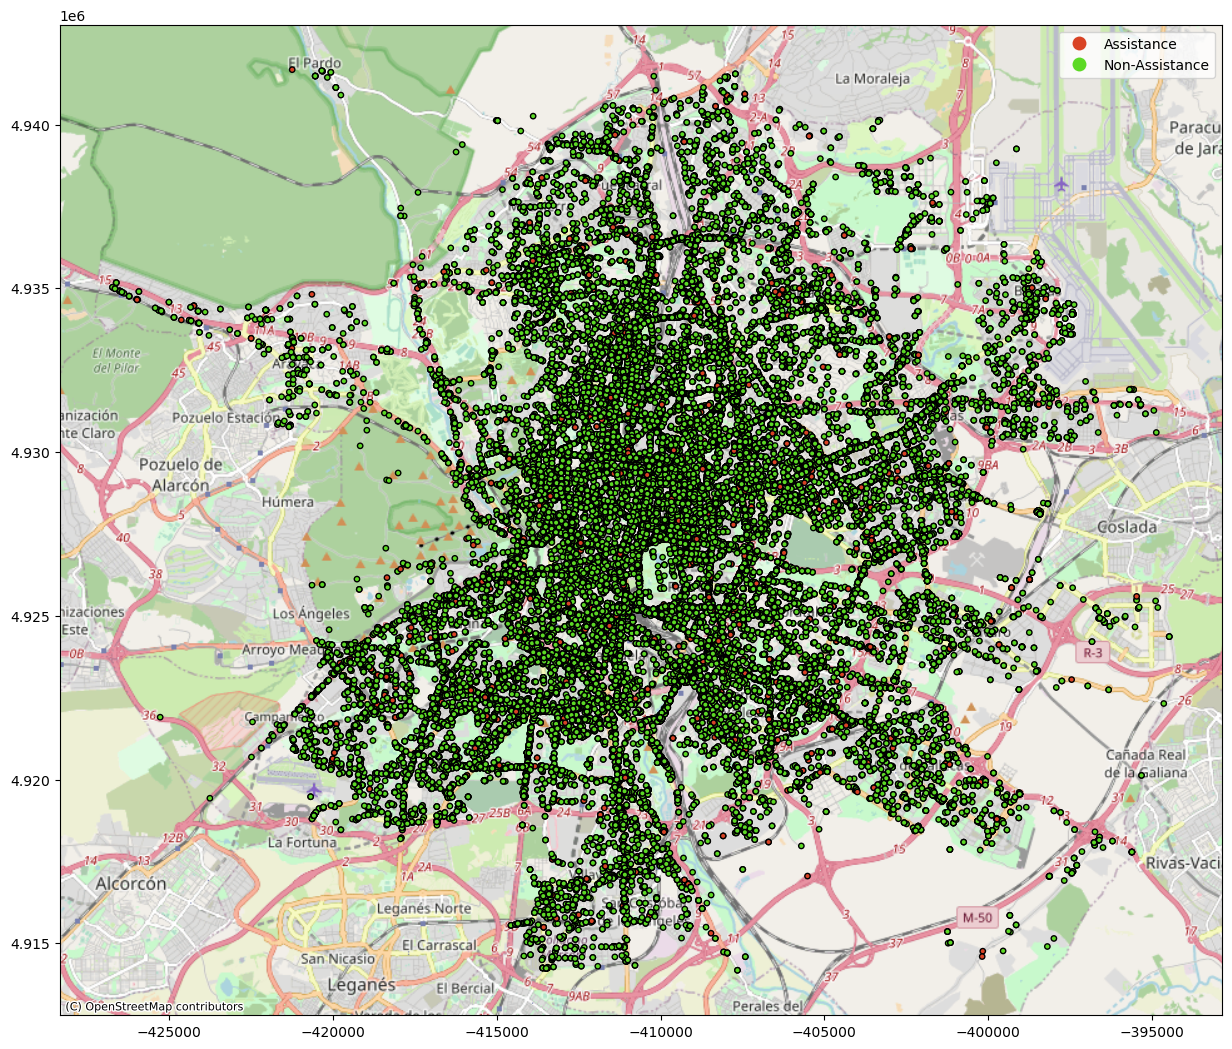
\includegraphics[width=90mm]{Figures/Madrid/original_OpenStreetMap.Mapnik.png}
		\label{MadridAccidentsMap:Original}
	}\\
	\subfloat[][Mapa de los accidentes filtrados de Madrid]{
		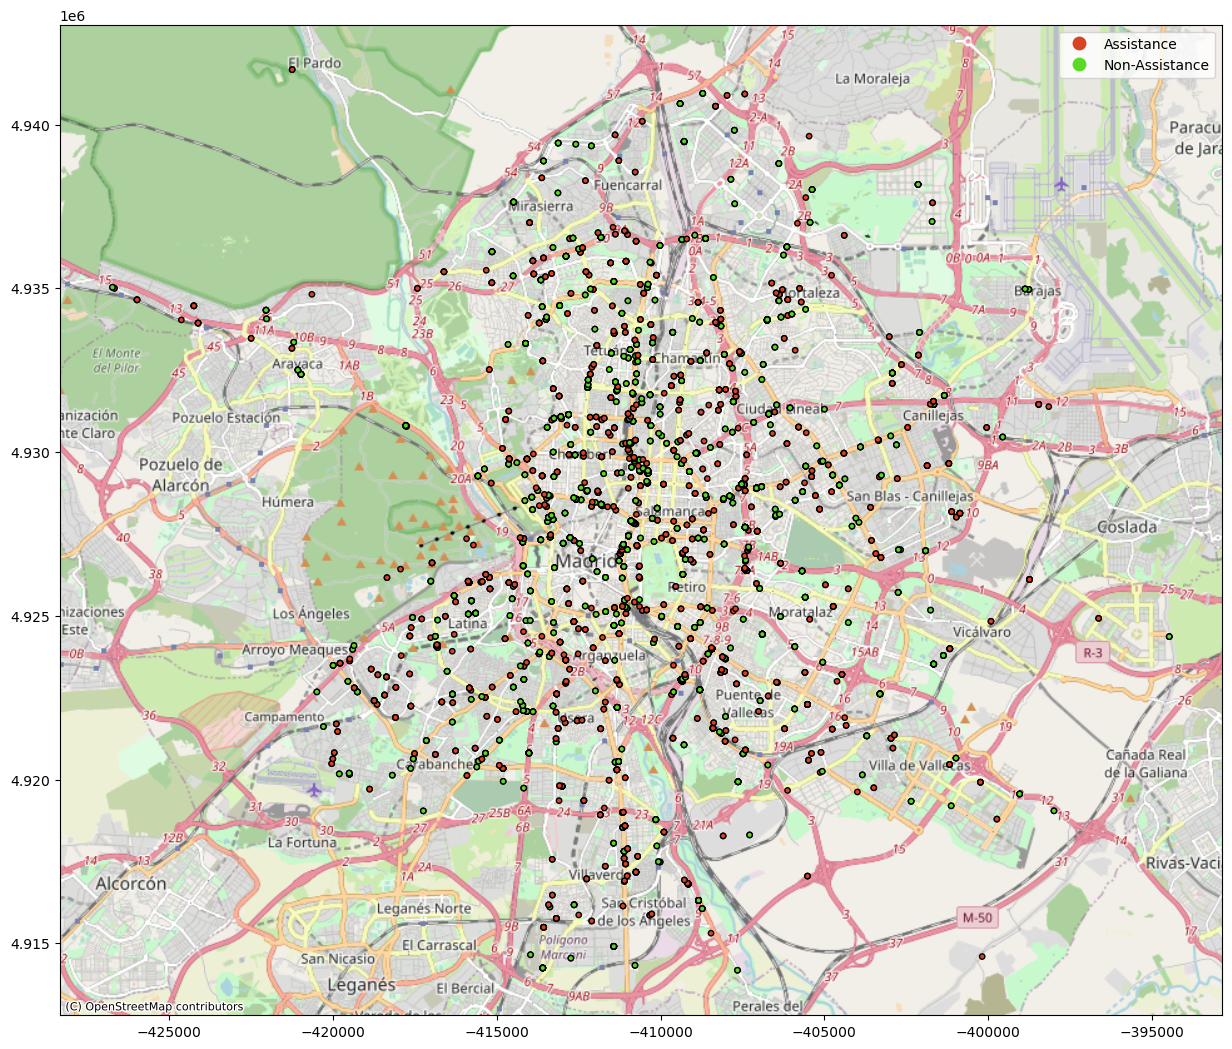
\includegraphics[width=90mm]{Figures/Madrid/filtered_OpenStreetMap.Mapnik.png}
		\label{MadridAccidentsMap:Filtered}
	}\\
	\caption{Mapa de accidentes de Madrid, original y filtrado}
	\label{MadridAccidentsMap}
\end{figure}

En la Figura \ref{MadridLossFunction} se muestra la evolución de la función a optimizar (\textit{F1-Score}) a lo largo de las 50 épocas para las que se ha entrenado el modelo GTAAF en la ciudad de Madrid. Se observa cómo el \textit{F1-Score} para el conjunto de entrenamiento sufre una evolución importante durante las diez primeras épocas, después de las cuales sigue aumentando en menor medida. Por otra parte, la métrica sobre el conjunto de validación sufre una evolución más lenta, hasta aproximadamente la época 30 no se ve una clara evolución en la generalización del modelo sobre datos que nunca ha visto.


\begin{figure}[h]
	\centering
	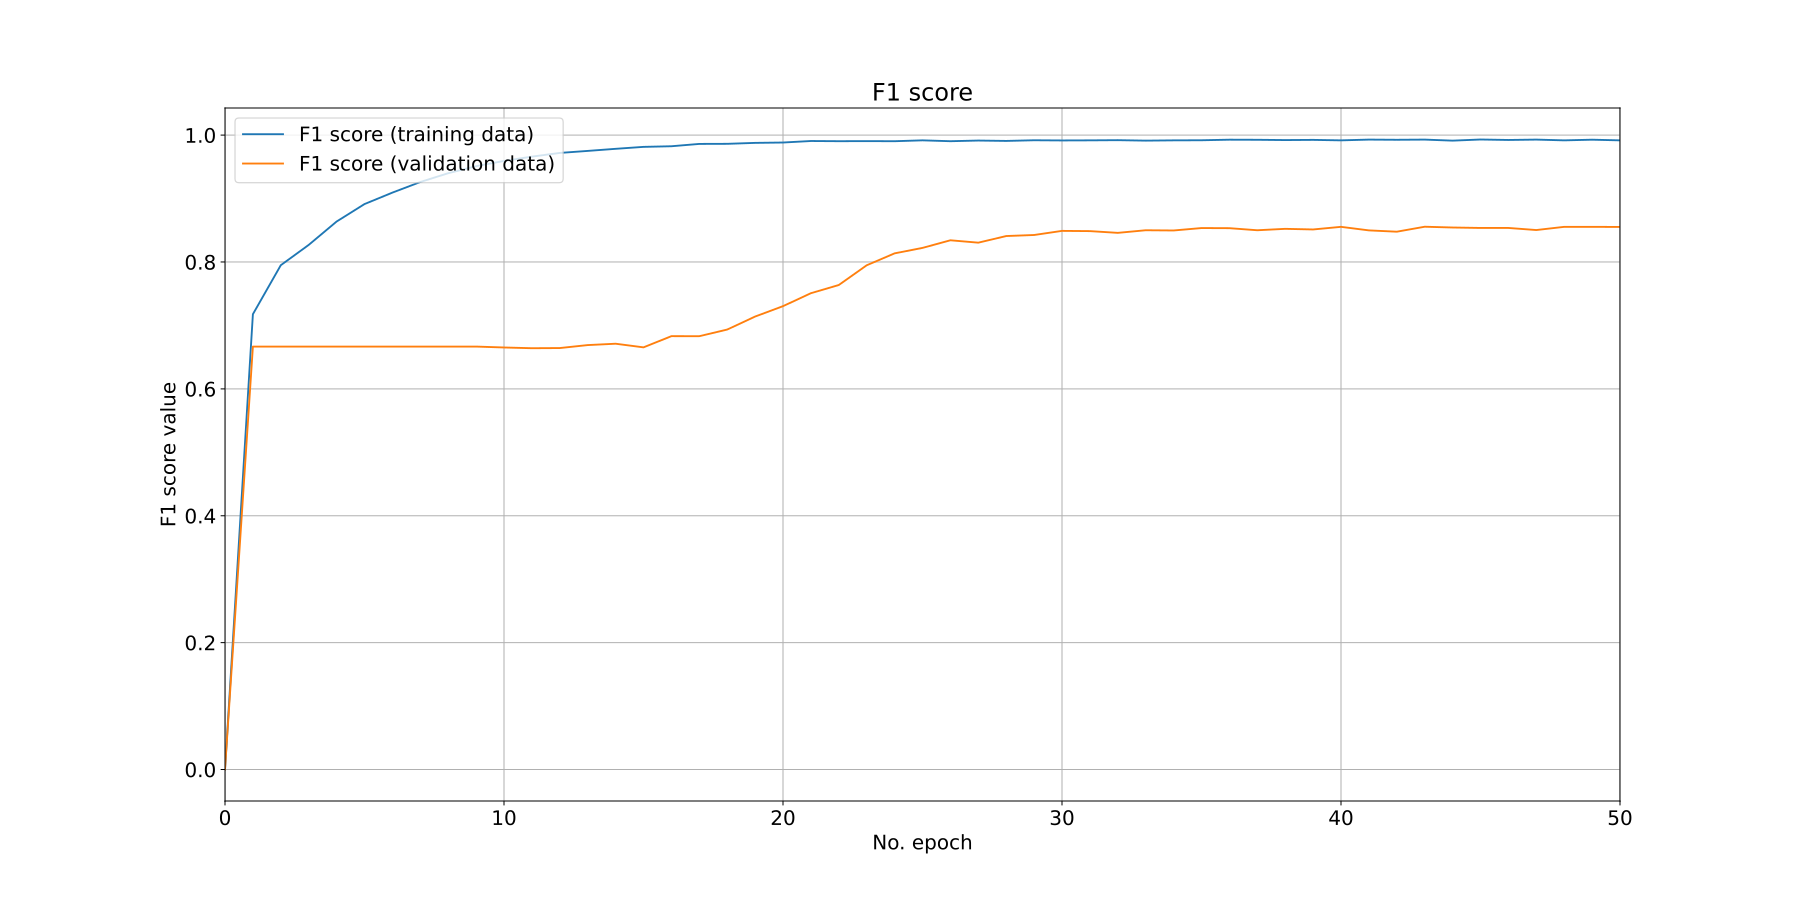
\includegraphics[width=14cm]{Figures/Madrid/madrid_convolution_2d_f1_score_2023-12-03-12 54 29.png}
	\caption{Evolución de \textit{F1-Score} del modelo GTAAF en Madrid}
	\label{MadridLossFunction}
\end{figure}

En la tabla \ref{SpainMetrics} se observan los resultados de la métrica \textit{F1-Score} de la predicción de la gravedad de los accidentes de cada uno de los modelos sobre el conjunto de test de la ciudad de Madrid. Como se puede comprobar, el valor más alto lo ofrece el nuevo modelo GTAAF, llegando a mejorar en un 3,9\% al siguiente mejor modelo, el \textit{SVC} sobre los accidentes Sin Asistencia, mientras que la mejora sobre los accidentes Con Asistencia se presenta en un 5,7\% sobre el siguiente modelo que mejor métricas ofrece, el \textit{SVC}. Con estos resultados se puede interpretar que el nuevo modelo GTAAF propuesto es capaz de generalizar mejor en la predicción de la gravedad de nuevos accidentes que no ha visto previamente sobre la ciudad de Madrid.

%%%%%%%%%%%%%%%%%%%%%%%%%%%%%%%%%%%%%%%%%%%%%%%%%%%%%%%%%%%%%%%%%%%%%%%%%%%%%%%%%
\begin{table}[H]
	\caption{\textit{F1-Score} por modelo y clase de accidente en Madrid (España)}
	\begin{center}
		\begin{tabular}{|c|c||c|c|c|c|c|c|}
			\hline
			\multicolumn{2}{ |c|| }{} &
			\multicolumn{1}{ |c| }{\textbf{\textit{F1-Score} España}} \\ \hline
			
			\textbf{Modelo} & \textbf{Asistencia} & Madrid
			\\ \hline \hline
			
			\multirow{2}{*}{NB} &
			No &  0.729 \\ &
			Sí & 0.621 \\ \hline \hline
			\multirow{2}{*}{SVC} &
			No & 0.862 \\ &
			Sí &  0.748 \\ \hline \hline
			\multirow{2}{*}{KNN} &
			No  & 0.739 \\ &
			Sí & 0.634 \\ \hline \hline
			\multirow{2}{*}{RF} &
			No & 0.744 \\ &
			Sí & 0.643  \\ \hline \hline
			\multirow{2}{*}{LR} &
			No &  0.750 \\ &
			Sí & 0.623 \\ \hline \hline
			\multirow{2}{*}{MLP} &
			No & 0.856 \\ &
			Sí & 0.724  \\ \hline \hline
			\multirow{2}{*}{\textbf{GTAAF}} &
			\textbf{No} & \textbf{0.894} \\ &
			\textbf{Sí} & \textbf{0.798} \\ \hline \hline
		\end{tabular}
	\end{center}

	\label{SpainMetrics}
\end{table}
%%%%%%%%%%%%%%%%%%%%%%%%%%%%%%%%%%%%%%%%%%%%%%%%%%%%%%%%%%%%%%%%%%%%%%%%%%%%%%%%%

\subsubsection*{Victoria}

En el segundo caso, tenemos una región dispersa, el estado de Victoria (Australia). Victoria, estado en Australia, abarca una región muy extensa y con gran diversidad, desde regiones desérticas hasta ciudades multitudinarias como Melbourne, situada a lo largo de la costa sureste. En la figura \ref{VictoriaAccidentsMap} se muestra la distribución de accidentes sobre la población de Victoria, aquellos Sin Asistencia se encuentran marcados en verde mientras que aquellos tipo Con Asistencia se encuentran representados en rojo. Como se puede observar en la figura \ref{VictoriaAccidentsMap:Original} gran parte de la concentración de los accidentes se encuentra sobre la ciudad de Melbourne y sus núcleos urbanos próximos (como Ballarat al oeste, Shepparton al norte o Traralgon al este), al igual que en las carreteras que conectan estas poblaciones. Al ser un estado extenso, el filtrado de áreas es más amplio, lo que resulta una variante respecto a ciudades de mayor concentración. En la Figura \ref{VictoriaAccidentsMap:Filtered} se observa la distribución de accidentes resultante tras aplicar el proceso de filtrado, donde aquellas zonas que presentan más accidentes Con Asistencia son en las grandes poblaciones y en las interconexiones entre estas.


\begin{figure}[H]
	\centering
	\subfloat[][Mapa de los accidentes originales de Victoria]{
		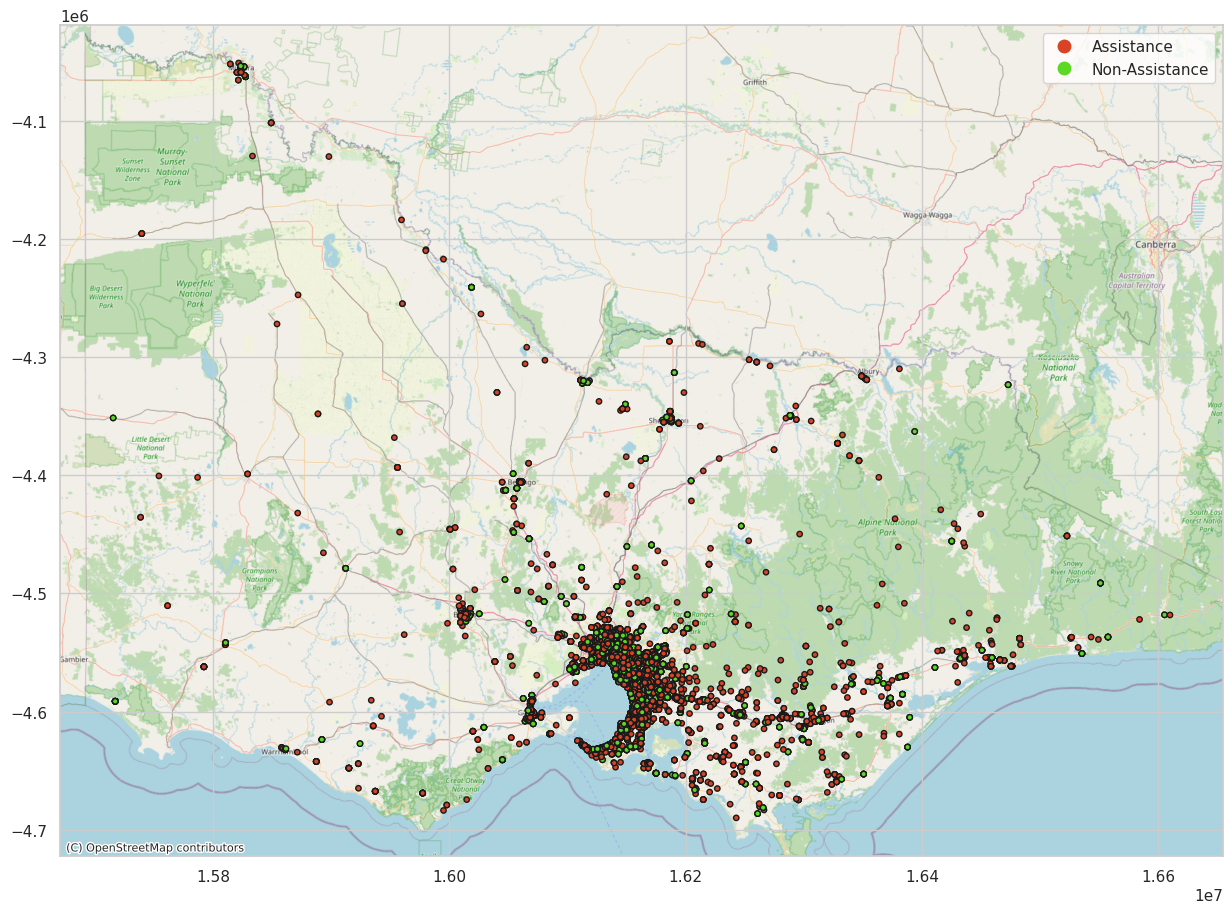
\includegraphics[width=120mm]{Figures/Victoria/original_OpenStreetMap.Mapnik.png}
		\label{VictoriaAccidentsMap:Original}
	}\\
	\subfloat[][Mapa de los accidentes filtrados de Victoria]{
		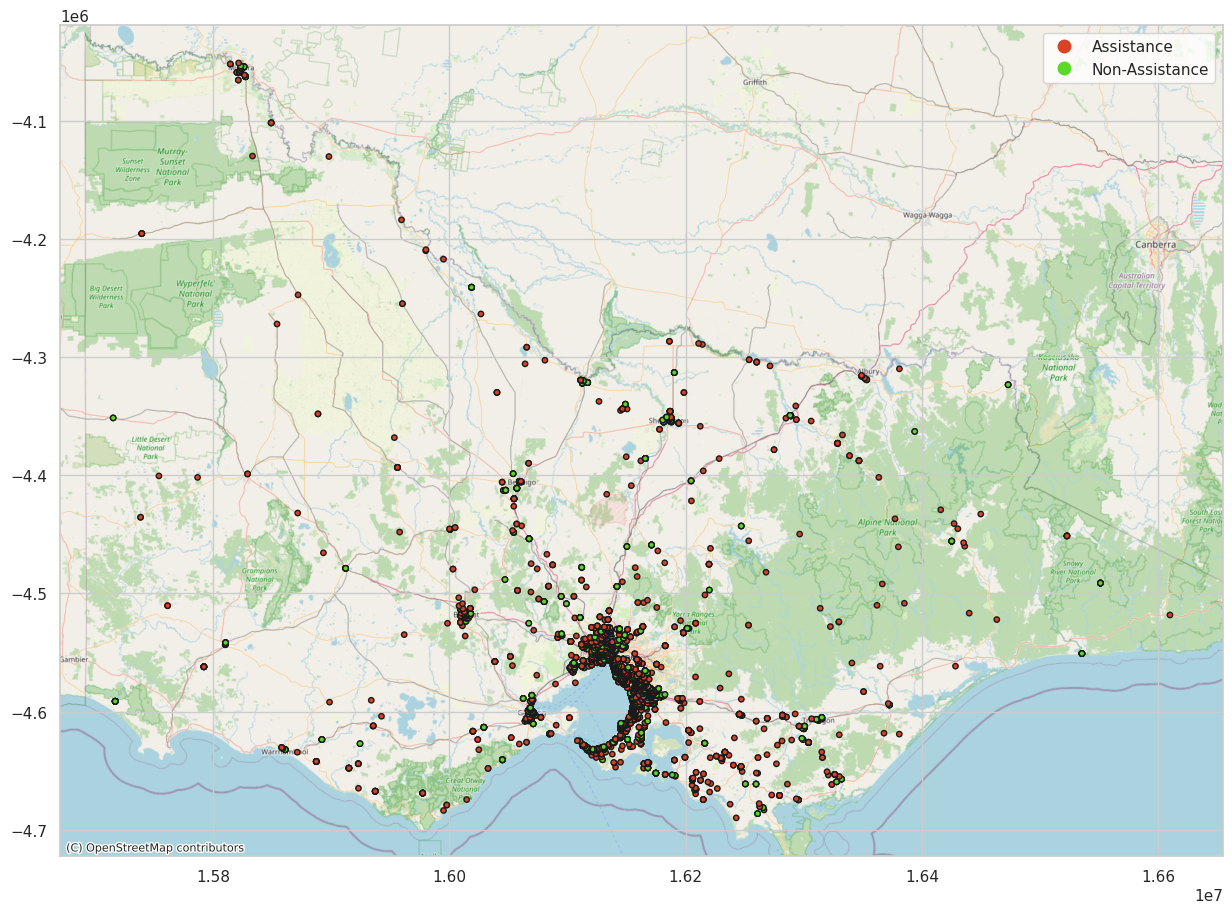
\includegraphics[width=120mm]{Figures/Victoria/filtered_OpenStreetMap.Mapnik.png}
		\label{VictoriaAccidentsMap:Filtered}
	}\\
	\caption{Mapa de accidentes de Victoria, original y filtrado.}
	\label{VictoriaAccidentsMap}
\end{figure}


En la Figura \ref{VictoriaLossFunction} se muestran las funciones \textit{F1-Score} sobre los datos de entrenamiento y validación para la región de Victoria. Esta métrica sobre el conjunto de entrenamiento muestra una curva de aprendizaje más lenta respecto a la anterior ciudad de Madrid, lo cual es comprensible ya que existe más variabilidad de datos en esta región al ser mucho más extensa que la anterior. La función de validación presenta más variaciones a lo largo del aprendizaje, llegando a su máximo aproximadamente en la época 45.

\begin{figure}[h!]
	\centering
	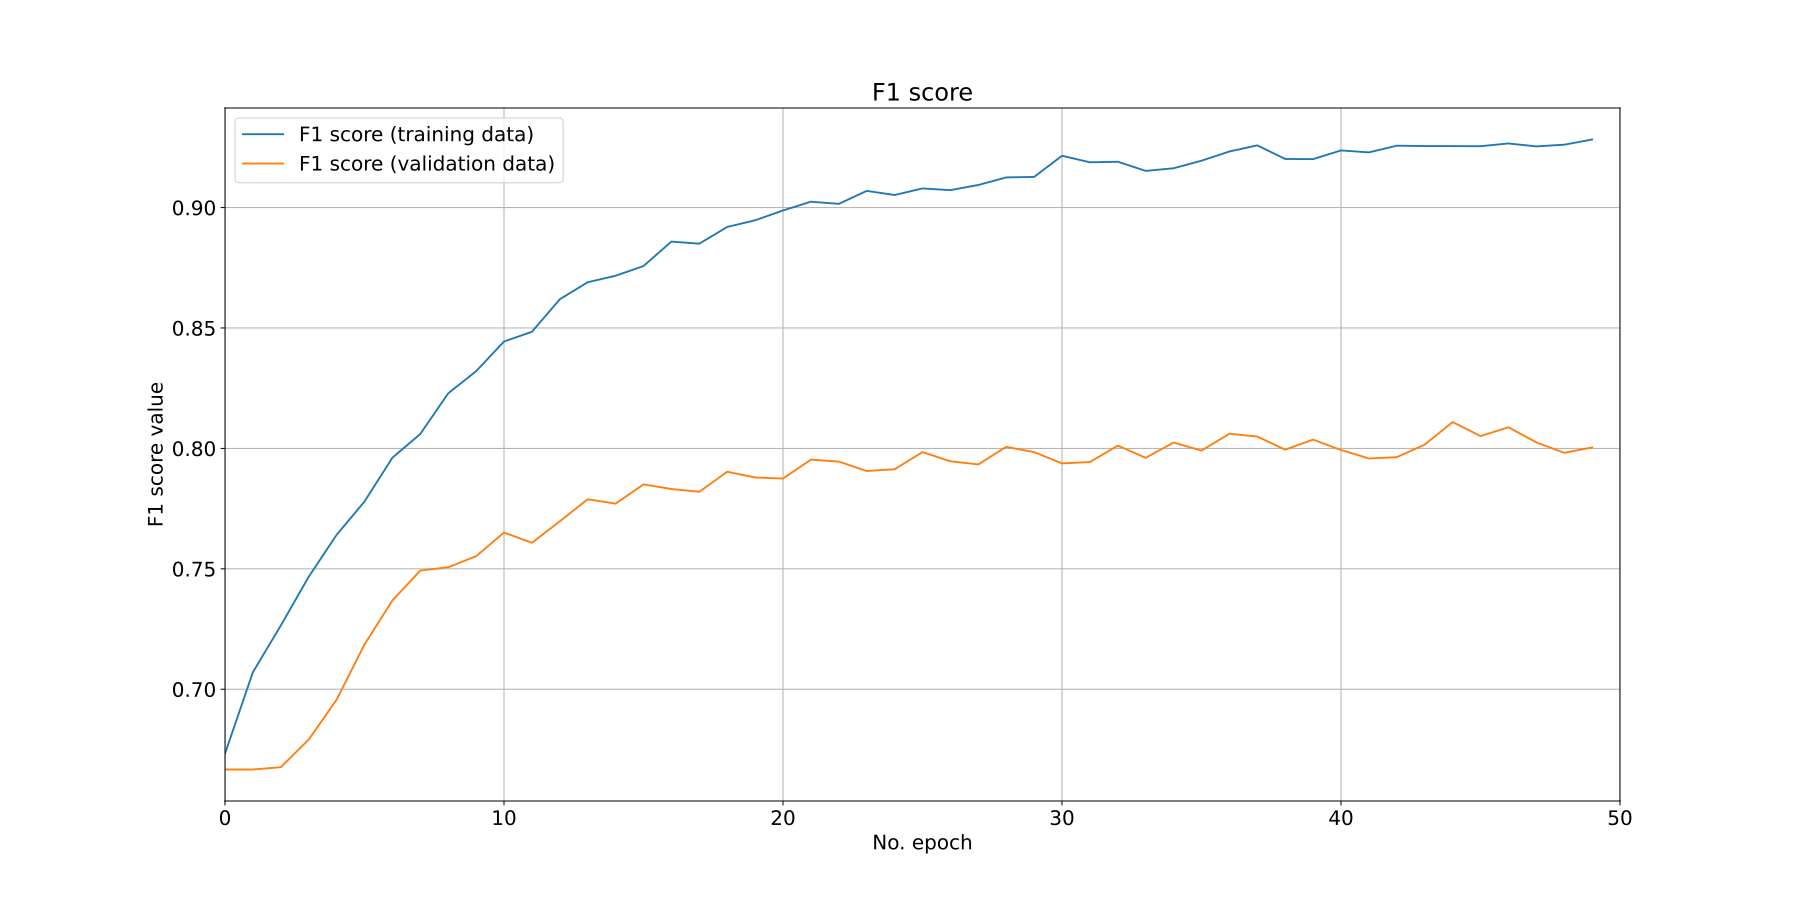
\includegraphics[width=14cm]{Figures/Victoria/Victoria_convolution_2d_f1_score_paper.png}
	\caption{Evolución de \textit{F1-Score} del modelo GTAAF en Victoria.}
	\label{VictoriaLossFunction}
\end{figure}

En la Tabla \ref{AustraliaMetrics}, se presentan los resultados del F1-Score obtenidos por cada uno de los modelos para ambos tipos de clasificación de accidentes. Concretamente, se observa que el nuevo modelo GTAAF logra una mejora del 6.5\% en comparación con el siguiente mejor modelo, el \textit{SVC}, para accidentes Sin Asistencia. Por otro lado, en lo que respecta a accidentes Con Asistencia, hay una mejora del 9\% en comparación con el \textit{MLP}. Estos resultados reflejan una mejora significativa en la capacidad de generalización del nuevo modelo propuesto.


%%%%%%%%%%%%%%%%%%%%%%%%%%%%%%%%%%%%%%%%%%%%%%%%%%%%%%%%%%%%%%%%%%%%%%%%%%%%%%%%%
\begin{table}[H]
	\caption{\textit{F1-Score} por modelo y clase de accidente en Victoria (Australia)}
	\begin{center}
		\begin{tabular}{|c|c||c|c|c|c|c|c|}
			\hline
			\multicolumn{2}{ |c|| }{} &
			\multicolumn{1}{ |c| }{\textbf{\textit{F1-Score} Australia}} \\ \hline
			
			\textbf{Modelo} & \textbf{Asistencia} & Victoria
			\\ \hline \hline
			
			\multirow{2}{*}{NB} &
			No &  0.635 \\ &
			Sí & 0.476 \\ \hline \hline
			\multirow{2}{*}{SVC} &
			No & 0.662 \\ &
			Sí &  0.679 \\ \hline \hline
			\multirow{2}{*}{KNN} &
			No  & 0.654 \\ &
			Sí & 0.616 \\ \hline \hline
			\multirow{2}{*}{RF} &
			No & 0.647 \\ &
			Sí & 0.364  \\ \hline \hline
			\multirow{2}{*}{LR} &
			No &  0.612 \\ &
			Sí & 0.630 \\ \hline \hline
			\multirow{2}{*}{MLP} &
			No & 0.635 \\ &
			Sí & 0.694 \\ \hline \hline
			\multirow{2}{*}{\textbf{GTAAF}} &
			\textbf{No} & \textbf{0.727} \\ &
			\textbf{Sí} & \textbf{0.784} \\ \hline \hline
		\end{tabular}
	\end{center}

	\label{AustraliaMetrics}
\end{table}
%%%%%%%%%%%%%%%%%%%%%%%%%%%%%%%%%%%%%%%%%%%%%%%%%%%%%%%%%%%%%%%%%%%%%%%%%%%%%%%%%

\subsubsection*{Reino Unido}

En este apartado se analizarán los datos proyectados sobre las distintas localidades escogidas de Reino Unido y sus respectivos resultados. Para ello en primer lugar se realizará un breve análisis de cada una de las regiones, posteriormente se interpretarán las evoluciones de los entrenamientos del modelo GTAAF para concluir con un análisis de resultados de los modelos aplicados sobre ellas.

\textbf{Southwark}\\

Southwark es un distrito de Londres situado en la orilla sur del río Támesis, con una alta densidad de población. En la Figura \ref{SouthwarkAccidentsMap} se observa la distribución de los accidentes a lo largo del municipio de Southwark. Analizando el conjunto de datos original, figura \ref{SouthwarkAccidentsMap:Original}, se observa que estos se producen a lo largo de las distintas vías que conectan el municipio con el centro neurálgico de la ciudad, hecho habitual al conectar zonas menos pobladas con lugares de trabajo y de ocio, mientras que la minoría de ellos se presentan en las calles circundantes. Observando la distribución de accidentes tras el proceso de filtrado por áreas (figura \ref{SouthwarkAccidentsMap:Filtered}) se acentúa este hecho, donde se observan que aquellos principales accidentes Con Asistencia se producen en estas vías. Por otra parte se muestra una concentración minoritaria de este tipo de accidentes en la zona de Dulwich (sur), en la intersección de la circunvalación \textit{S Circular} red con la carretera que dirige al centro del municipio.

%%%%%%%%%%%%%%%%%%%%%%%% DESCOMENTAR %%%%%%%%%%%%%%%%%%%%%%%%

\begin{figure}[H]
	\centering
	\subfloat[][Mapa de los accidentes originales de Southwark]{
		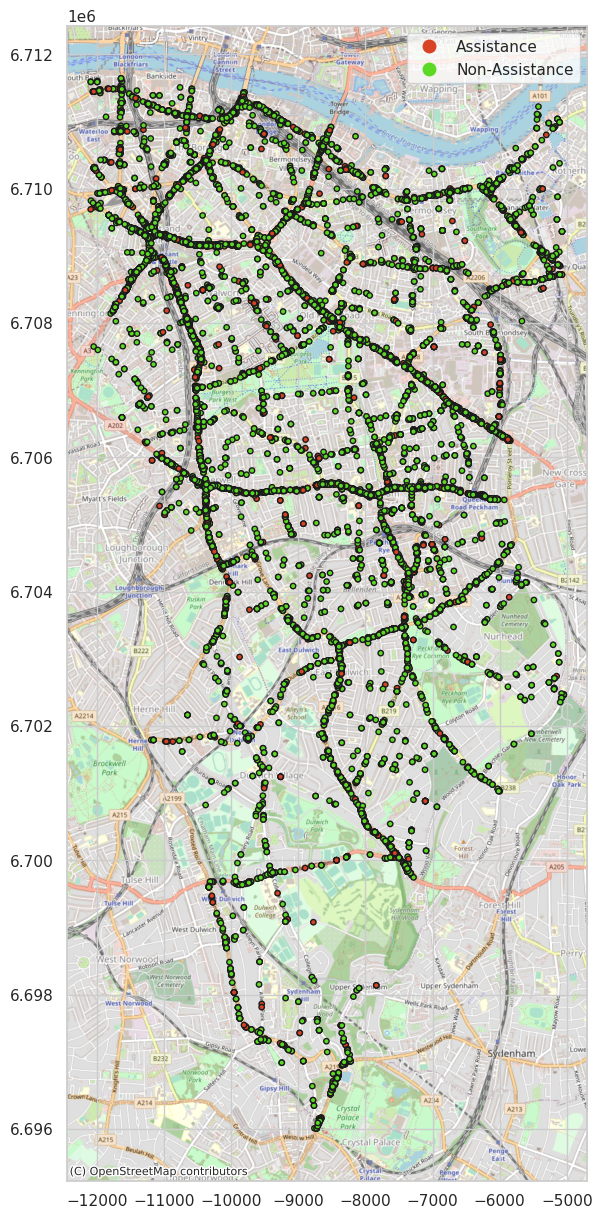
\includegraphics[width=70mm]{Figures/Southwark/original_OpenStreetMap.Mapnik.png}
		\label{SouthwarkAccidentsMap:Original}
	}
	\subfloat[][Mapa de los accidentes filtrados de Southwark]{
		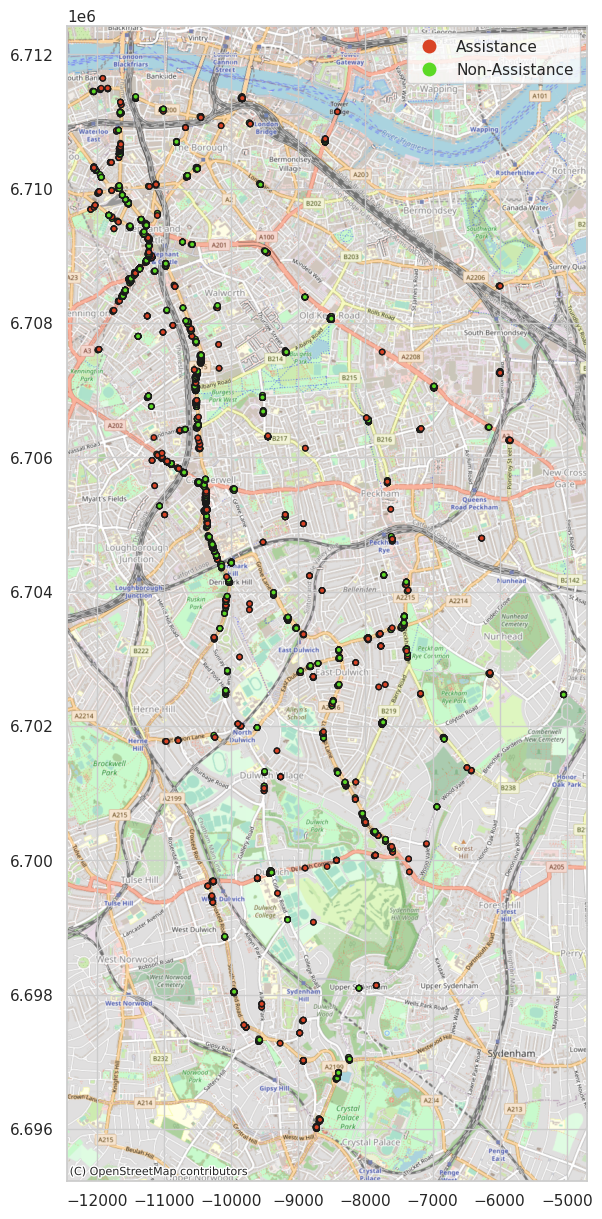
\includegraphics[width=70mm]{Figures/Southwark/filtered_OpenStreetMap.Mapnik.png}
		\label{SouthwarkAccidentsMap:Filtered}
	}
	\caption{Mapa de accidentes de Southwark, original y filtrado}
	\label{SouthwarkAccidentsMap}
\end{figure}


\textbf{Manchester}\\

Manchester, ubicada en el noroeste de Inglaterra, es una gran ciudad conocida por su legado industrial y su alta densidad de población. En la figura \ref{ManchesterAccidentsMap} se muestra la distribución de los accidentes de Manchester. Atendiendo a su distribución original, en la figura \ref{ManchesterAccidentsMap:Original}, como es habitual en cualquier población se aprecia una concentración de accidentes importante en la zona central de la ciudad, siendo también considerable en el área de Longsight. Por otra parte, las principales vías que comunican las periferias urbanas (norte) con el centro de la ciudad también presentan una concentración mayor de accidentes, lo que puede deberse a desplazamientos por motivos laborales o de ocio. Por otra parte, la carretera de Wythenshawe, cercano a Sale Water Park (Sur), también presenta una concentración elevada de accidentes, motivados por los desplazamientos de residencias personales. En la figura \ref{ManchesterAccidentsMap:Filtered} se observa la localización de los accidentes una vez se ha aplicado el proceso de filtrado por áreas, donde se vislumbra que gran parte de los accidentes Sin Asistencia se distribuyen a lo largo de las carreteras que comunican hacia el centro de la ciudad.

%%%%%%%%%%%%%%%%%%%%%%%% DESCOMENTAR %%%%%%%%%%%%%%%%%%%%%%%%

\begin{figure}[H]
	\centering
	\subfloat[][Mapa de los accidentes originales de Manchester]{
		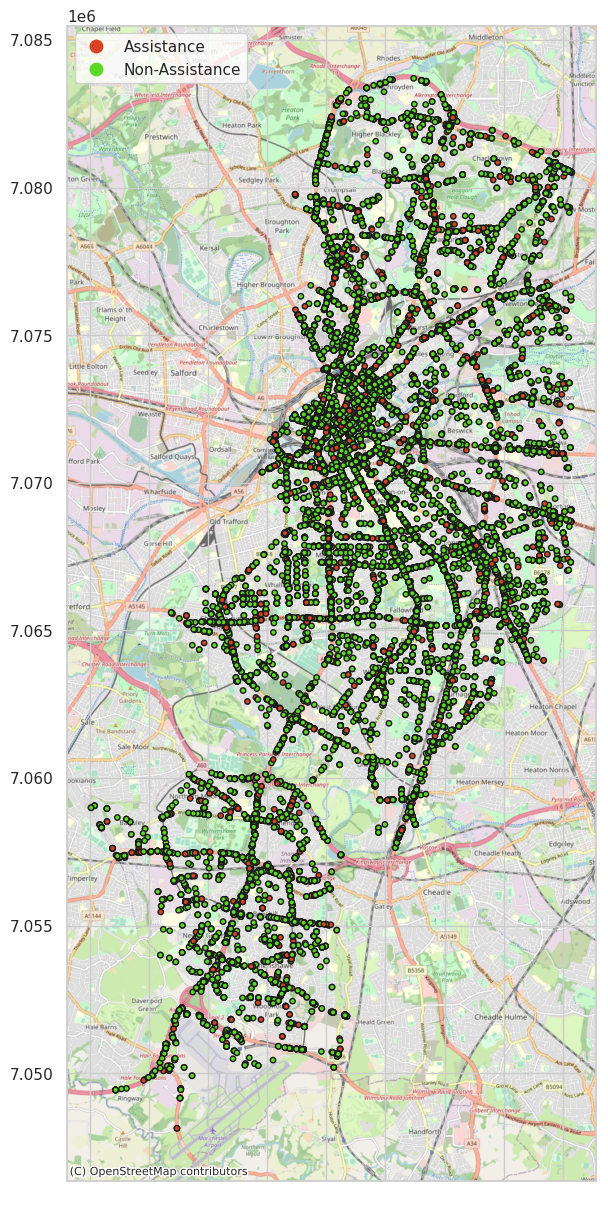
\includegraphics[width=70mm]{Figures/Manchester/original_OpenStreetMap.Mapnik.png}
		\label{ManchesterAccidentsMap:Original}
	}
	\subfloat[][Mapa de los accidentes filtrados de Manchester]{
		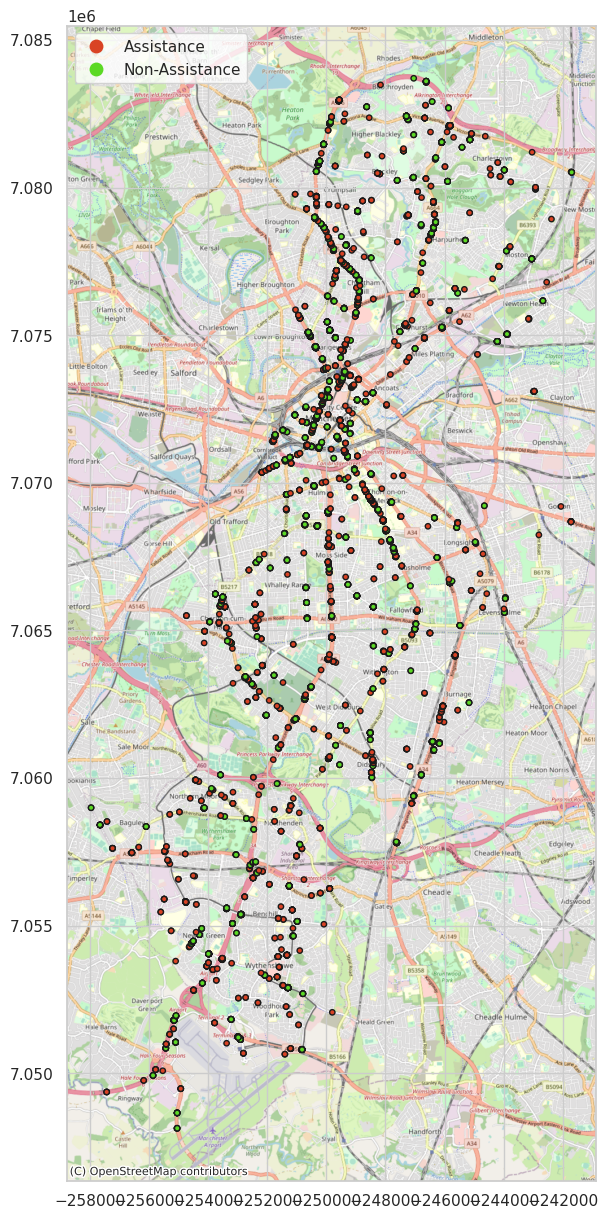
\includegraphics[width=70mm]{Figures/Manchester/filtered_OpenStreetMap.Mapnik.png}
		\label{ManchesterAccidentsMap:Filtered}
	}
	\caption{Mapa de accidentes de Manchester, original y filtrado}
	\label{ManchesterAccidentsMap}
\end{figure}

\textbf{Birmingham}\\

Birmingham es la segunda ciudad más grande de Inglaterra, se extiende por West Midlands con un panorama urbano diverso y una densidad de población considerable, famosa por su historia industrial y su vitalidad cultural. En la figura \ref{BirminghamAccidentsMap} se muestra la distribución de los accidentes de Birmingham, tanto los originales como los resultantes una vez aplicado el proceso de filtrado. Como se puede observar en los accidentes originales en la Figura \ref{BirminghamAccidentsMap:Original} se aprecia que gran parte de estos se concentran en la zona centro de la ciudad, una  tendencia normal debido a que es el principal foco de actividad de las ciudades. Mientras que los accidentes se van dispersando a medida que distan de este punto. Se aprecian ligeras agrupaciones de accidentes a lo largo de las zonas de incorporaciones a las principales arterias de la ciudad, como es al este, el caso de Handsworth. Por otra parte, en la figura \ref{BirminghamAccidentsMap:Filtered} se muestran los accidentes una vez se ha aplicado el proceso de filtrado por áreas. Como se puede observar, la información ha sido resumida sin dar lugar a pérdidas de valor en ella. Se visualizan ciertas zonas más conflictivas donde se producen accidentes más importantes, como es el caso de la carretera Holyhead Rd de entrada a la ciudad o en Northfield.

%%%%%%%%%%%%%%%%%%%%%%%% DESCOMENTAR %%%%%%%%%%%%%%%%%%%%%%%%

\begin{figure}[H]
	\centering
	\subfloat[][Mapa de los accidentes originales de Birmingham]{
		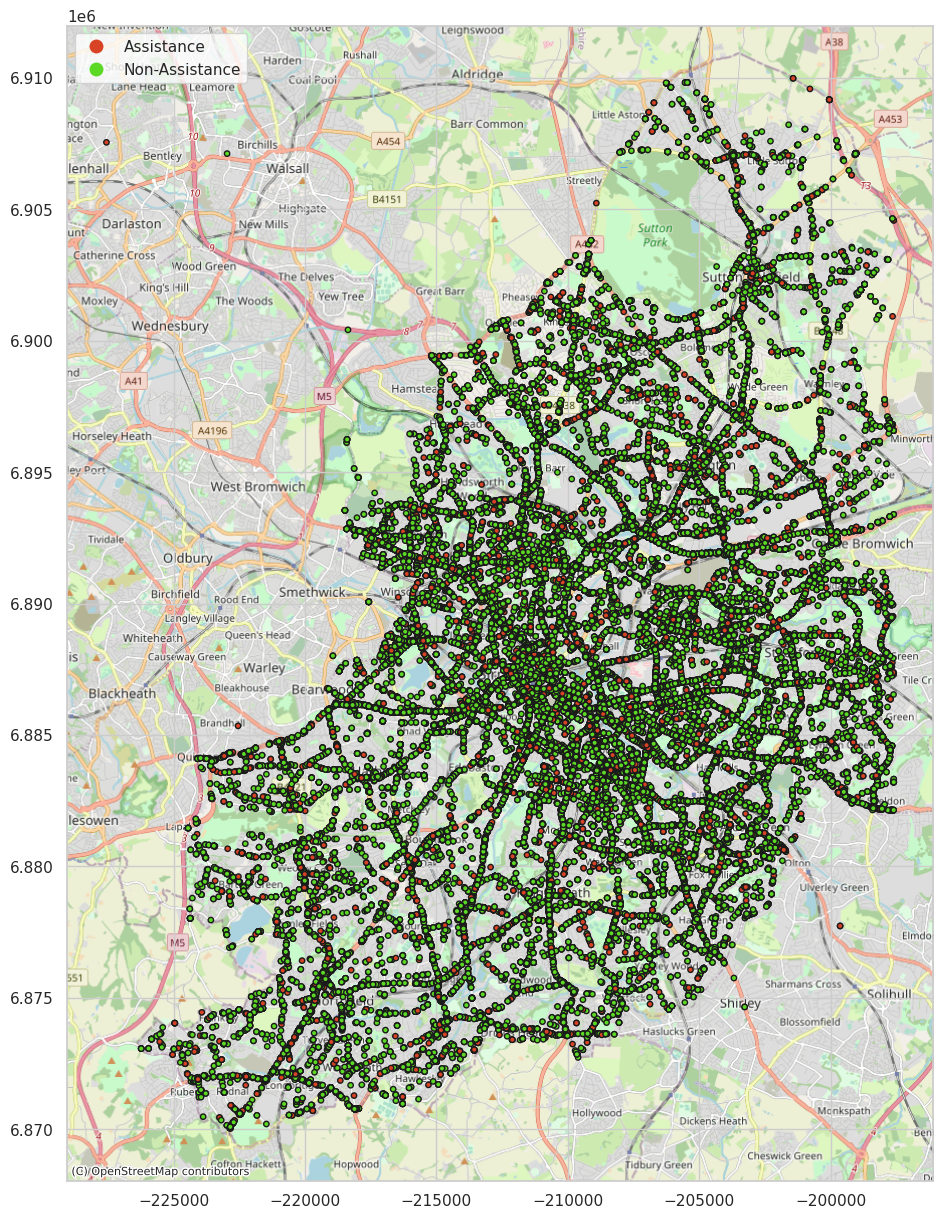
\includegraphics[width=70mm]{Figures/Birmingham/original_OpenStreetMap.Mapnik.png}
		\label{BirminghamAccidentsMap:Original}
	}
	\subfloat[][Mapa de los accidentes filtrados de Birmingham]{
		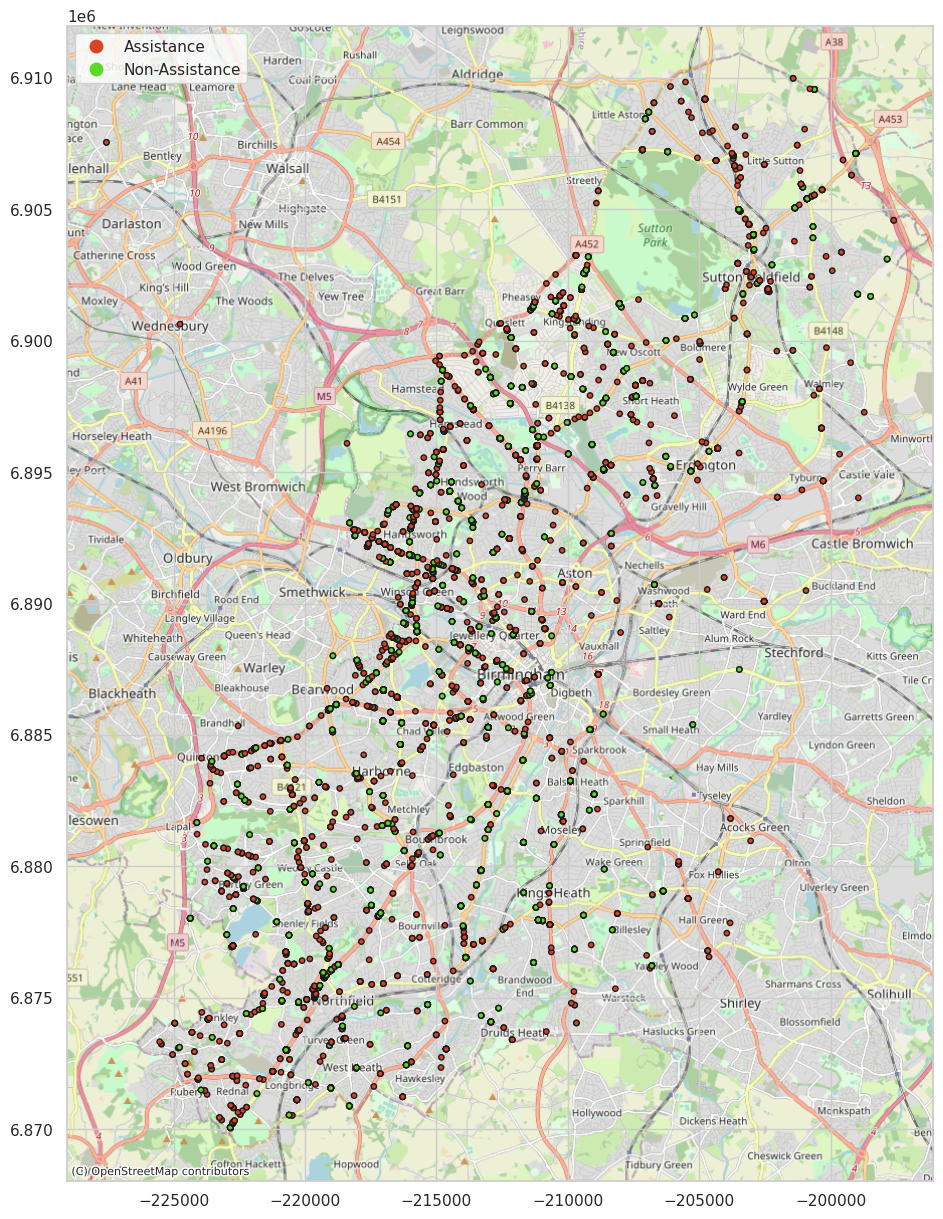
\includegraphics[width=70mm]{Figures/Birmingham/filtered_OpenStreetMap.Mapnik.png}
		\label{BirminghamAccidentsMap:Filtered}
	}
	\caption{Mapa de accidentes de Birmingham, original y filtrado}
	\label{BirminghamAccidentsMap}
\end{figure}


\textbf{Liverpool}\\

Liverpool, ubicada a lo largo del río Mersey en el noroeste de Inglaterra, prospera como una ciudad marítima con una rica historia, profundidad cultural y una densidad de población significativa, reconocida por su encanto en el frente marítimo y su legado musical. En la figura \ref{LiverpoolAccidentsMap} se muestra la comparativa de la distribución de accidentes originales del conjunto de datos y aquellos filtrados para esta ciudad. En la figura \ref{LiverpoolAccidentsMap:Original} se aprecian accidentes concentrados en la zona centro de la ciudad, como viene siendo habitual, además de a lo largo de las circunvalaciones que la rodean. En la figura \ref{LiverpoolAccidentsMap:Filtered}, después del proceso de filtrado, se aprecia que gran parte de los accidentes Con Asistencia se producen a lo largo de Strand Street (desde el sur hasta el oeste), convergiendo ambas direcciones en el centro neurálgico. Por otra parte se visualiza otra concentración en la carretera que conecta la localidad de Ormskirk con el centro (noroeste), una de las principales vías de conexión.

%%%%%%%%%%%%%%%%%%%%%%%% DESCOMENTAR %%%%%%%%%%%%%%%%%%%%%%%%


\begin{figure}[H]
	\centering
	\subfloat[][Mapa de los accidentes originales de Liverpool]{
		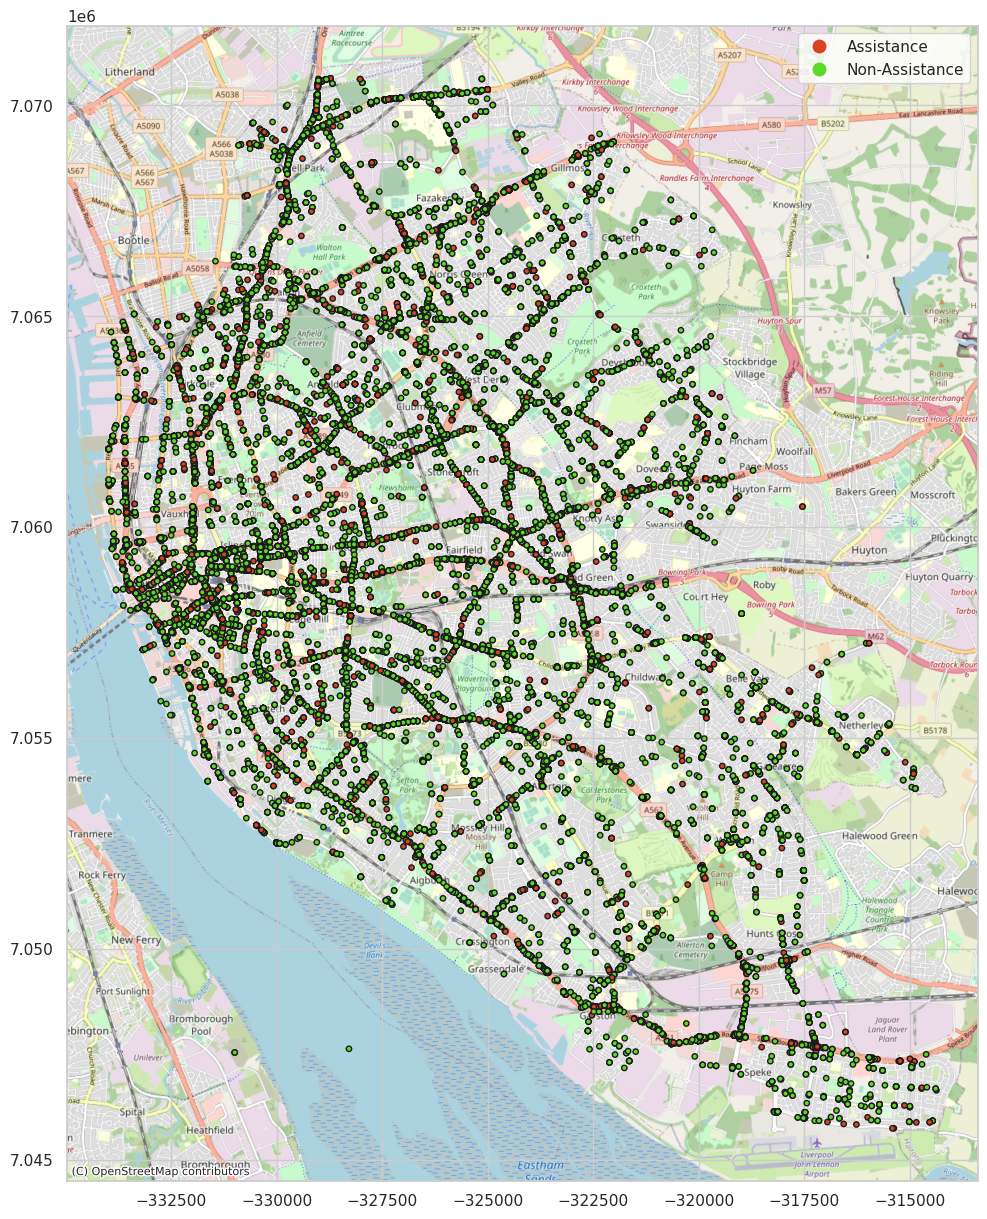
\includegraphics[width=70mm]{Figures/Liverpool/original_OpenStreetMap.Mapnik.png}
		\label{LiverpoolAccidentsMap:Original}
	}
	\subfloat[][Mapa de los accidentes filtrados de Liverpool]{
		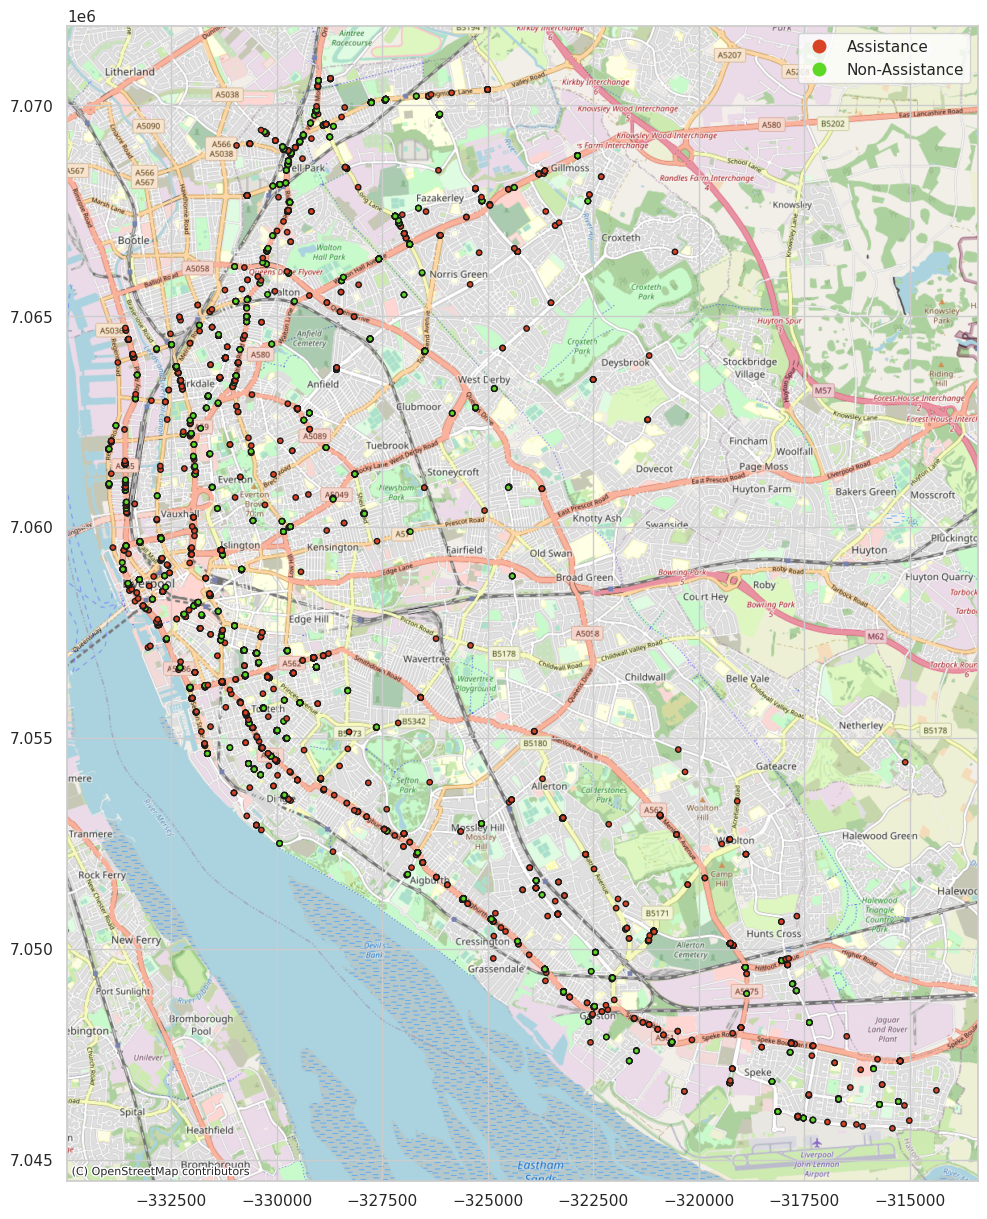
\includegraphics[width=70mm]{Figures/Liverpool/filtered_OpenStreetMap.Mapnik.png}
		\label{LiverpoolAccidentsMap:Filtered}
	}
	\caption{Mapa de accidentes de Liverpool, original y filtrado}
	\label{LiverpoolAccidentsMap}
\end{figure}

\textbf{Sheffield}\\

Sheffield, ubicada en South Yorkshire, presume de un patrimonio industrial y paisajes pintorescos, con una densidad de población intermedia. En la figura \ref{SheffieldAccidentsMap} se muestra la distribución de accidentes para la ciudad, tanto la original como la resultante tras la etapa de filtrado. En la figura \ref{SheffieldAccidentsMap:Original} se pueden apreciar distintas concentraciones en zonas estratégicas. Como suele ser habitual, el núcleo urbano es un centro de mayor densidad de incidentes, mientras que en las intersecciones que conectan la ciudad de Sheffield y la de Rotherham (cruces de Tinsley Viaduct con Meadow Bank Road y la \textit{A6178}, al noreste de Sheffield). También se aprecian concentraciones en los suburbios de Wadsley Bridge y Malin Bridge, periferias de la ciudad, además de alrededor de todas las vías principales que conectan con el centro. Por otra parte, en la figura \ref{SheffieldAccidentsMap:Filtered} se muestran los accidentes una vez se ha realizado el proceso de filtrado, donde se aprecia que aquellos que han requerido de asistencia normalmente se presentan en las principales arterias, donde se circula a una mayor velocidad.

%%%%%%%%%%%%%%%%%%%%%%%% DESCOMENTAR %%%%%%%%%%%%%%%%%%%%%%%%

\begin{figure}[H]
	\centering
	\subfloat[][Mapa de los accidentes originales de Sheffield]{
		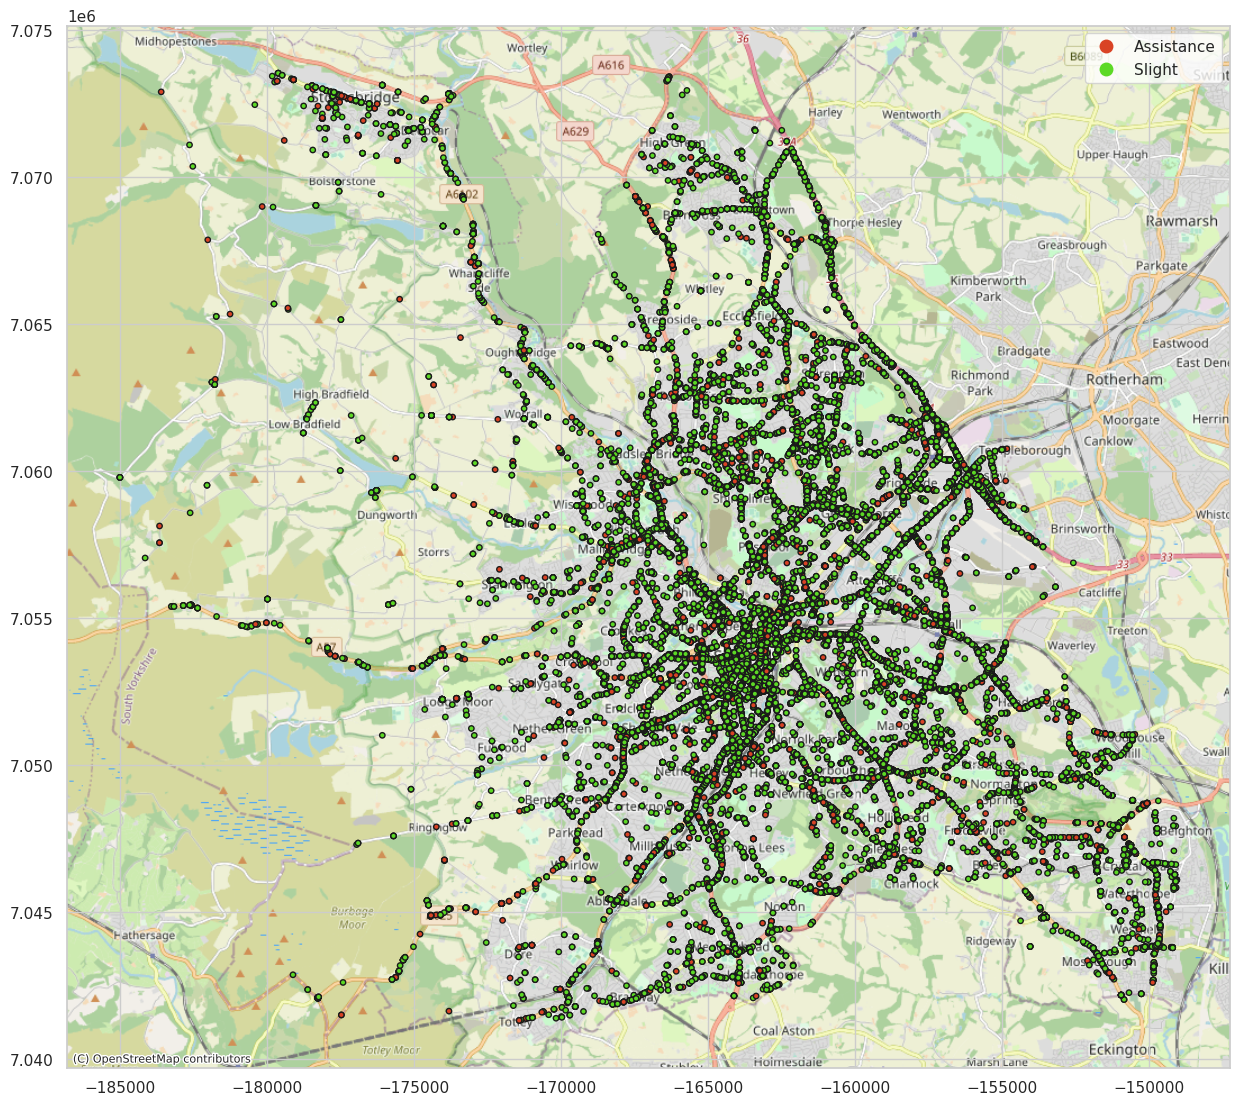
\includegraphics[width=75mm]{Figures/Sheffield/original_OpenStreetMap.Mapnik.png}
		\label{SheffieldAccidentsMap:Original}
	}
	\subfloat[][Mapa de los accidentes filtrados de Sheffield]{
		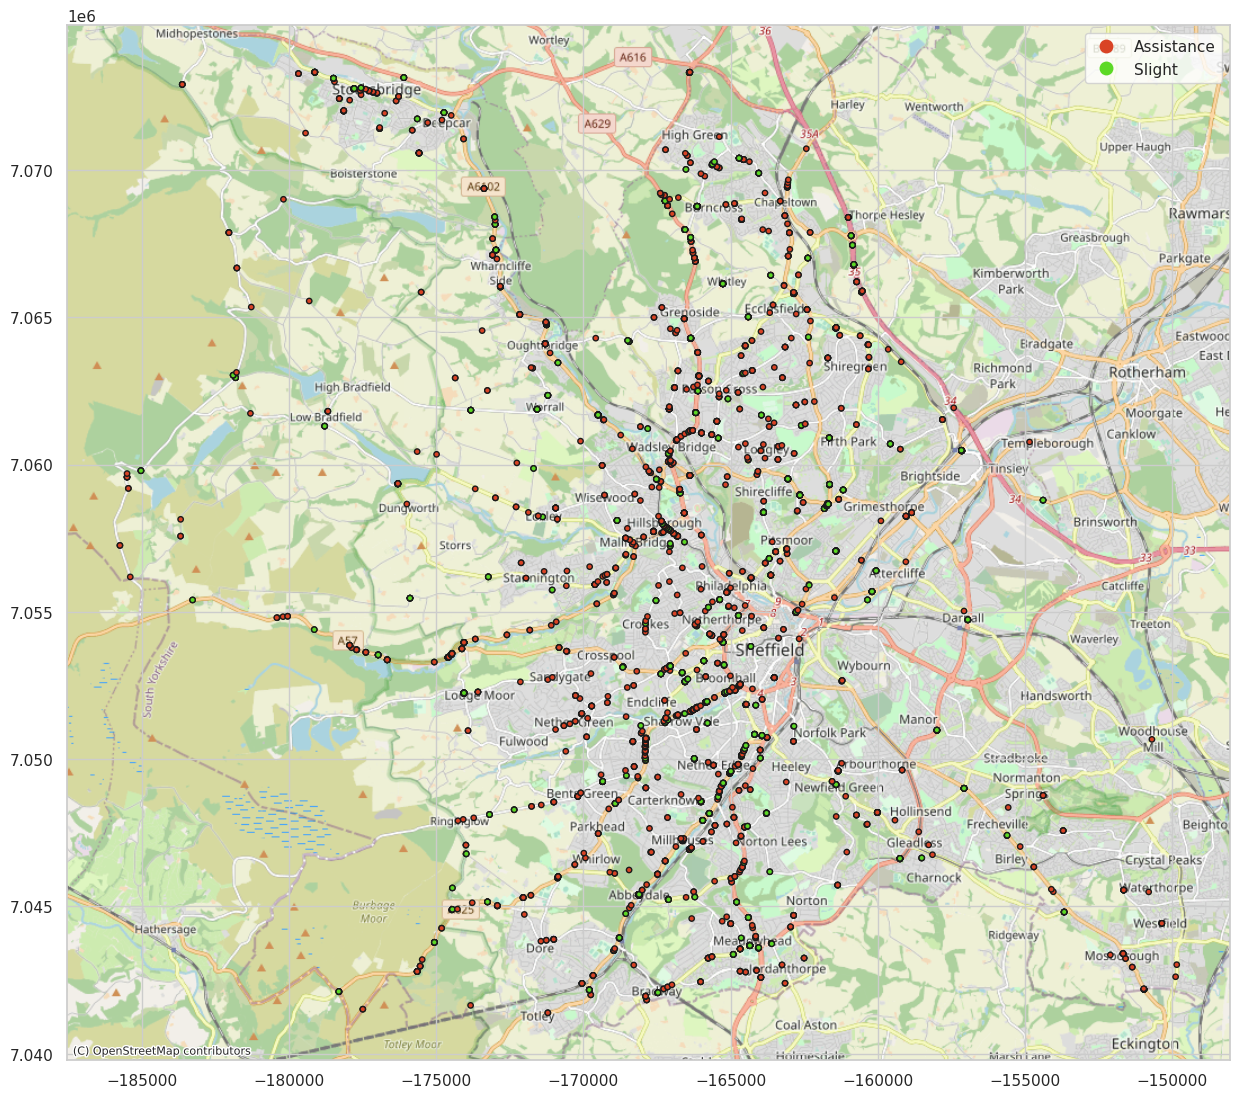
\includegraphics[width=75mm]{Figures/Sheffield/filtered_OpenStreetMap.Mapnik.png}
		\label{SheffieldAccidentsMap:Filtered}
	}
	\caption{Mapa de accidentes de Sheffield, original y filtrado}
	\label{SheffieldAccidentsMap}
\end{figure}


\textbf{Cornwall}\\

Cornwall, situada en la parte suroeste de Inglaterra con sus apacibles paisajes, encantadores pueblos costeros y extensiones rurales, fomenta un entorno tranquilo alejado de los núcleos de alta densidad de población. En la Figura \ref{CornwallAccidentsMap} se muestran de nuevo los accidentes originales de dataset y los que resultan tras aplicar el proceso de filtrado sobre el condado de Cornwall. En la Figura \ref{CornwallAccidentsMap:Original} las principales concentraciones de accidentes se encuentran distribuidas a lo largo de las distintas ciudades del condado. La mayoría de estos se encuentran divididos en dos regiones claramente definidas, la primera de ellas entre las vías que conectan las localidades de Camborne y Redruth (suroeste de Cornwall), y el área comprendida entre St Austell, Duporth, Carlyon Bay y Par, este del condado. No obstante, el resto de regiones también presentan una concentración considerable, como es el caso de la ciudad de Falmouth (sureste), las localidades de Penzance y Hayle (suroeste), en la ciudad de Newquay y sus alrededores (oeste), Bodmin (centro) y Launceston (norte). De nuevo, en este caso, se demuestra que la mayor frecuencia de accidentes se presenta entre los principales núcleos de población y las carreteras que los interconectan, debido a que las grandes ciudades implican más movimientos de vehículos. Atendiendo a la Figura \ref{CornwallAccidentsMap:Filtered} se observa que la ocurrencia de accidentes Con Asistencia, una vez aplicado el proceso de filtrado, tiene la misma tendencia que el expuesto para el conjunto de datos original, distribuyéndose a lo largo de las principales carreteras del condado Cornwall y concentrándose más en los núcleos de población.

%%%%%%%%%%%%%%%%%%%%%%%% DESCOMENTAR %%%%%%%%%%%%%%%%%%%%%%%%


\begin{figure}[H]
	\centering
	\subfloat[][Mapa de los accidentes originales de Cornwall]{
		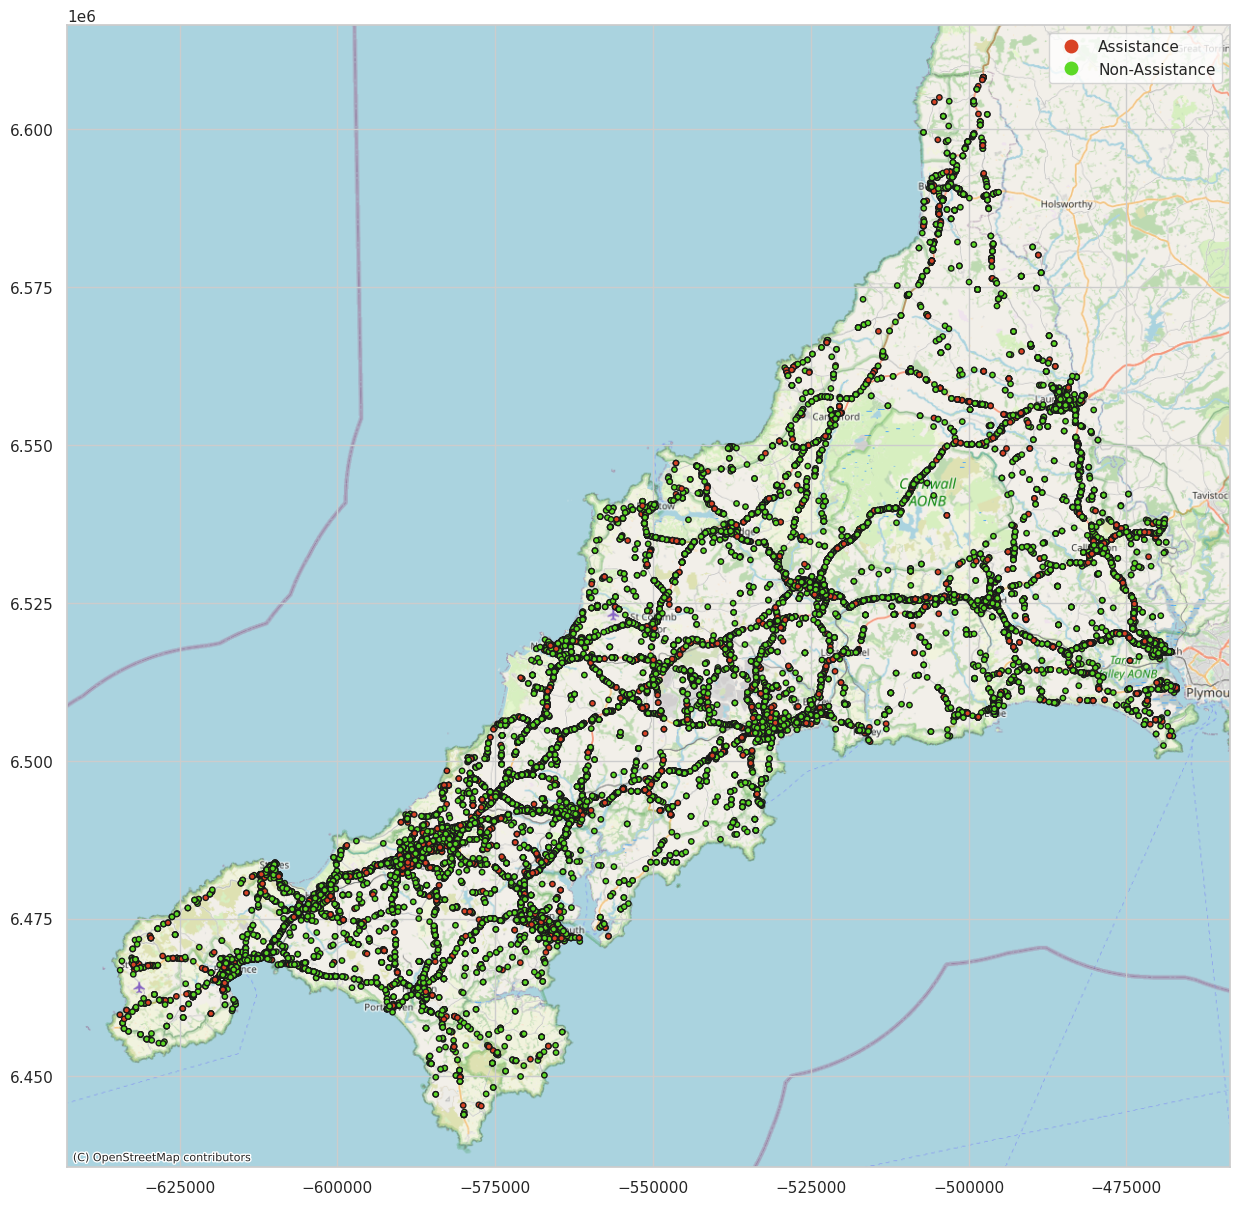
\includegraphics[width=90mm]{Figures/Cornwall/original_OpenStreetMap.Mapnik.png}
		\label{CornwallAccidentsMap:Original}
	}\\
	\subfloat[][Mapa de los accidentes filtrados de Cornwall]{
		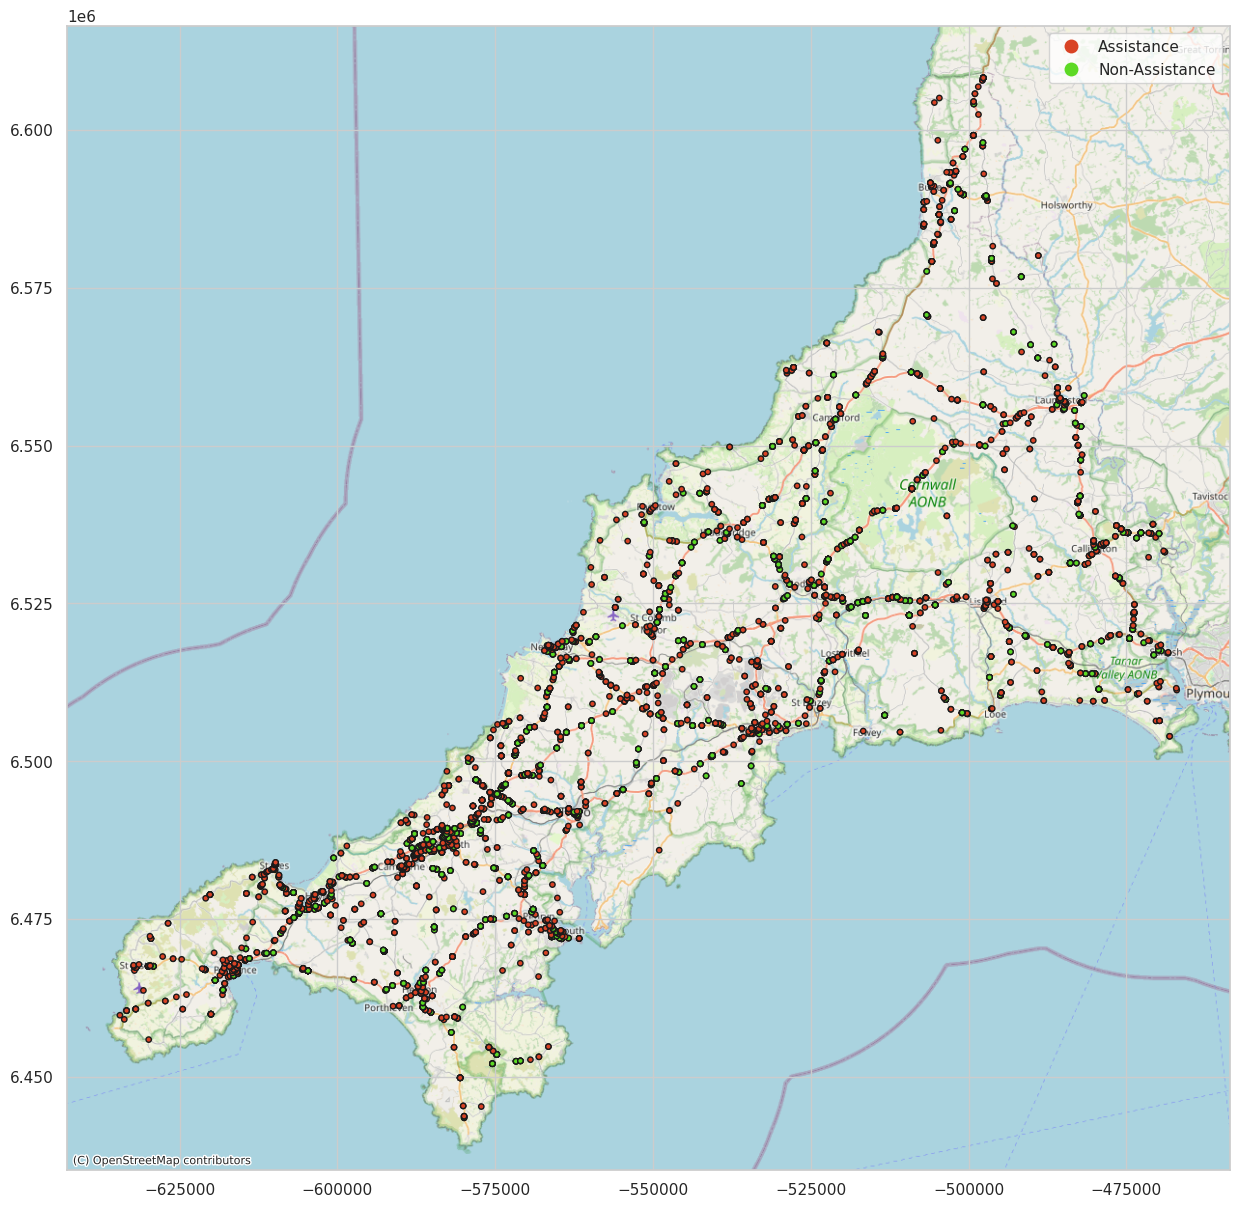
\includegraphics[width=90mm]{Figures/Cornwall/filtered_OpenStreetMap.Mapnik.png}
		\label{CornwallAccidentsMap:Filtered}
	}
	\caption{Mapa de accidentes de Cornwall, original y filtrado}
	\label{CornwallAccidentsMap}
\end{figure}

%%%%%%%%%%%%%%%%%%%%%%%% DESCOMENTAR %%%%%%%%%%%%%%%%%%%%%%%%

\textcolor{orange}{\textbf{LUIS: AQUÍ QUÉ COMENTAMOS?}}

\begin{figure}[H]
	\centering
	\subfloat[][Entrenamiento GTAAF en Southwark]{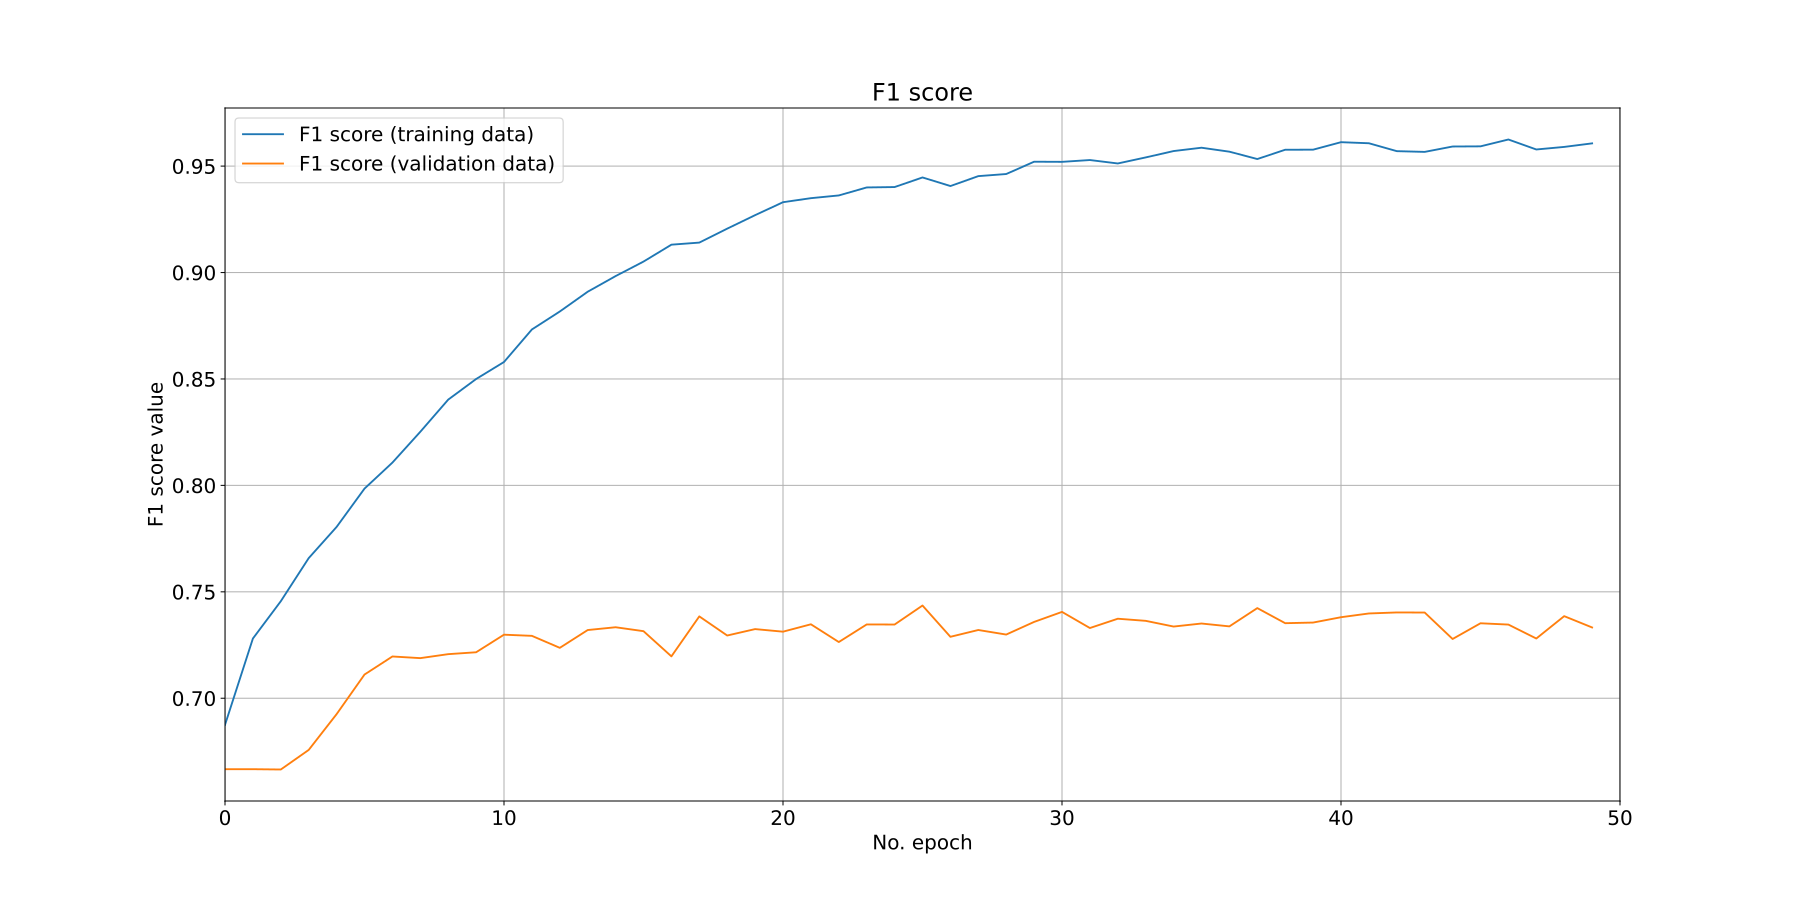
\includegraphics[width=80mm]{Figures/Cornwall/Cornwall_convolution_2d_f1_score_paper.png}}
	\subfloat[][Entrenamiento GTAAF en Manchester]{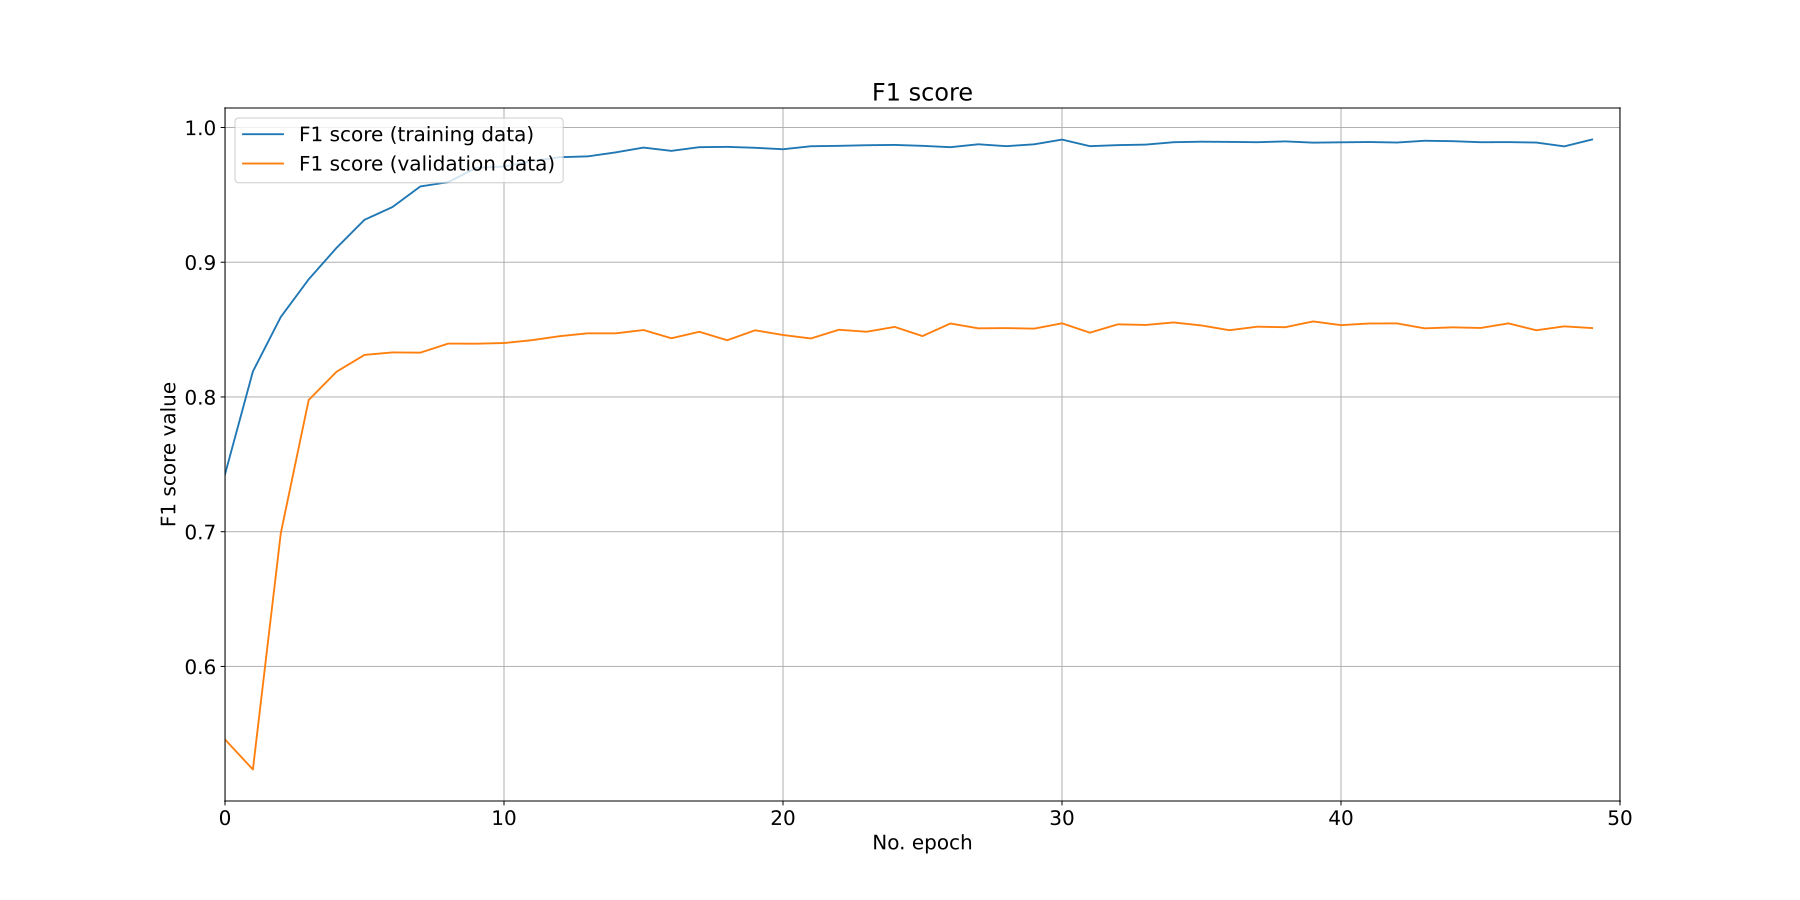
\includegraphics[width=80mm]{Figures/Manchester/Manchester_convolution_2d_f1_score_paper.png}}\\
	\subfloat[][Entrenamiento GTAAF en Birmingham]{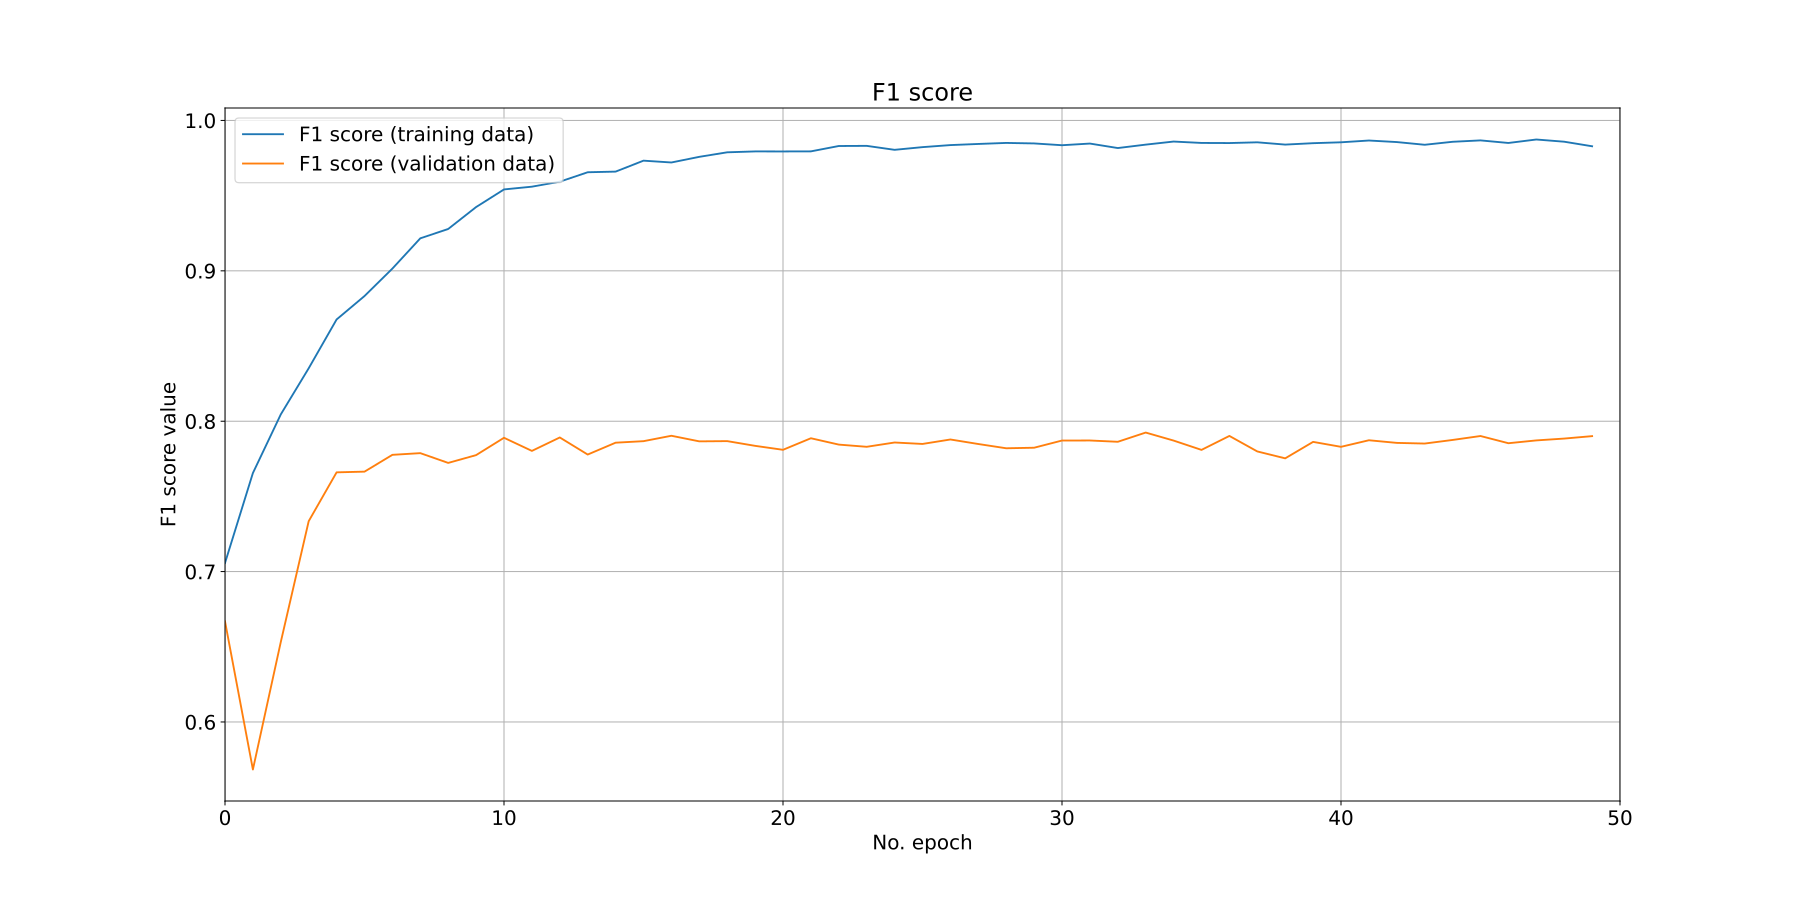
\includegraphics[width=80mm]{Figures/Birmingham/Birmingham_convolution_2d_f1_score_paper.png}}
	\subfloat[][Entrenamiento GTAAF en Liverpool]{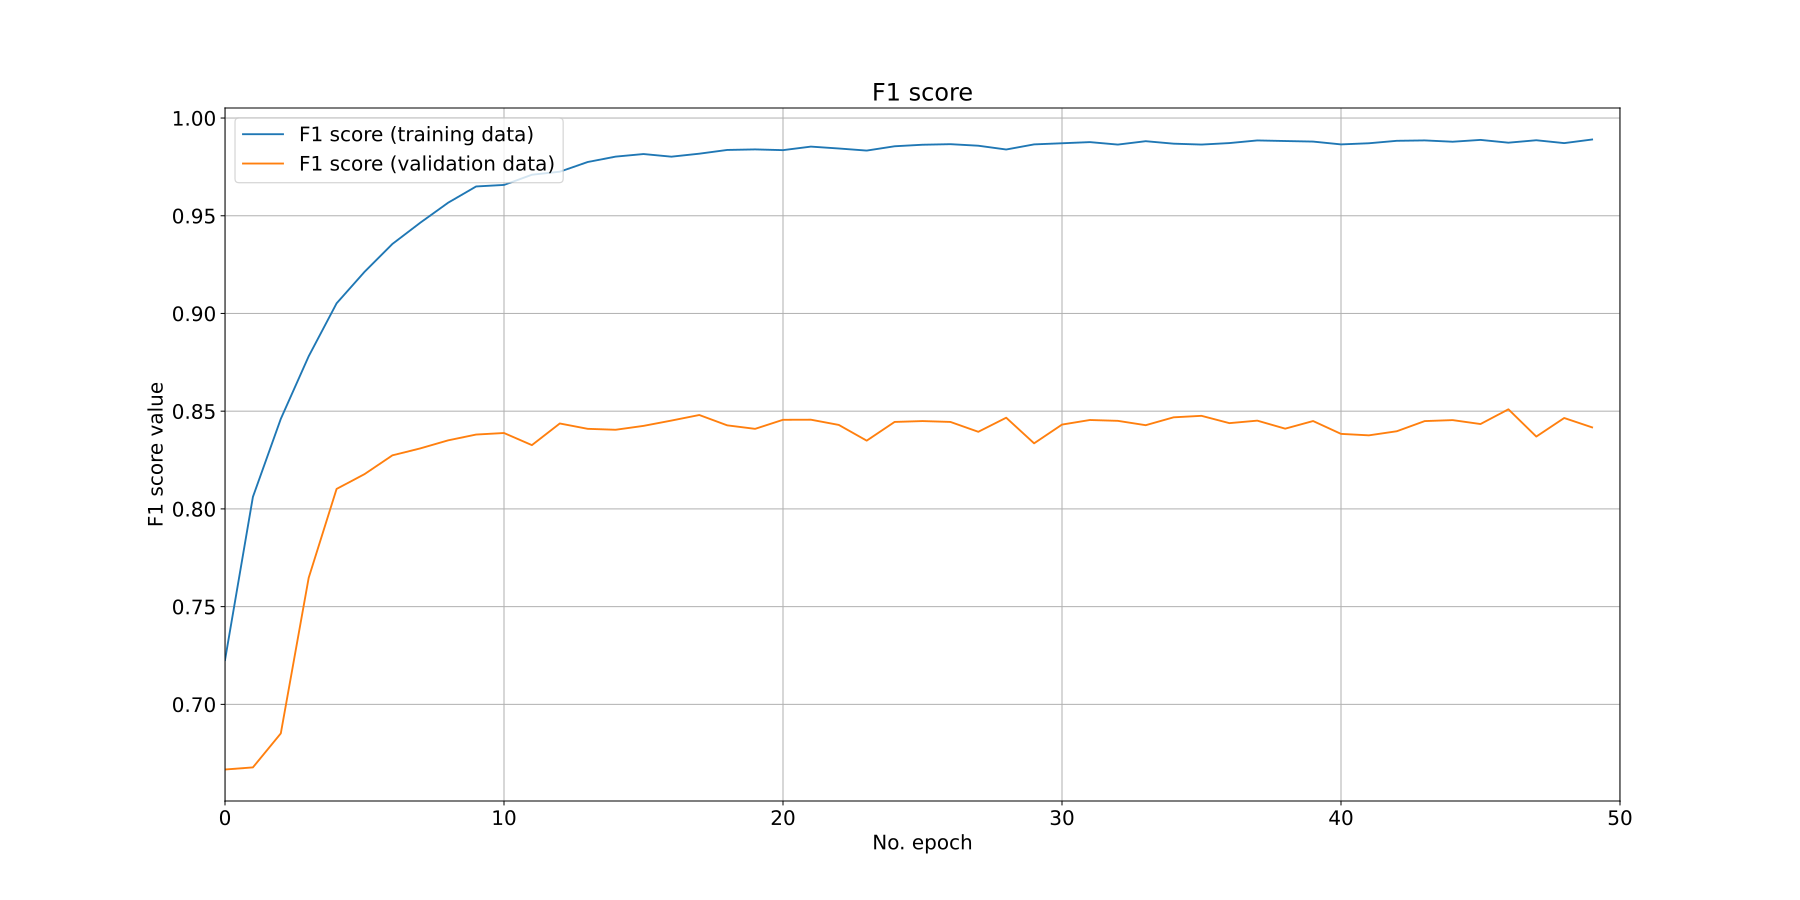
\includegraphics[width=80mm]{Figures/Liverpool/Liverpool_convolution_2d_f1_score_paper.png}}\\
	\subfloat[][Entrenamiento GTAAF en Sheffield]{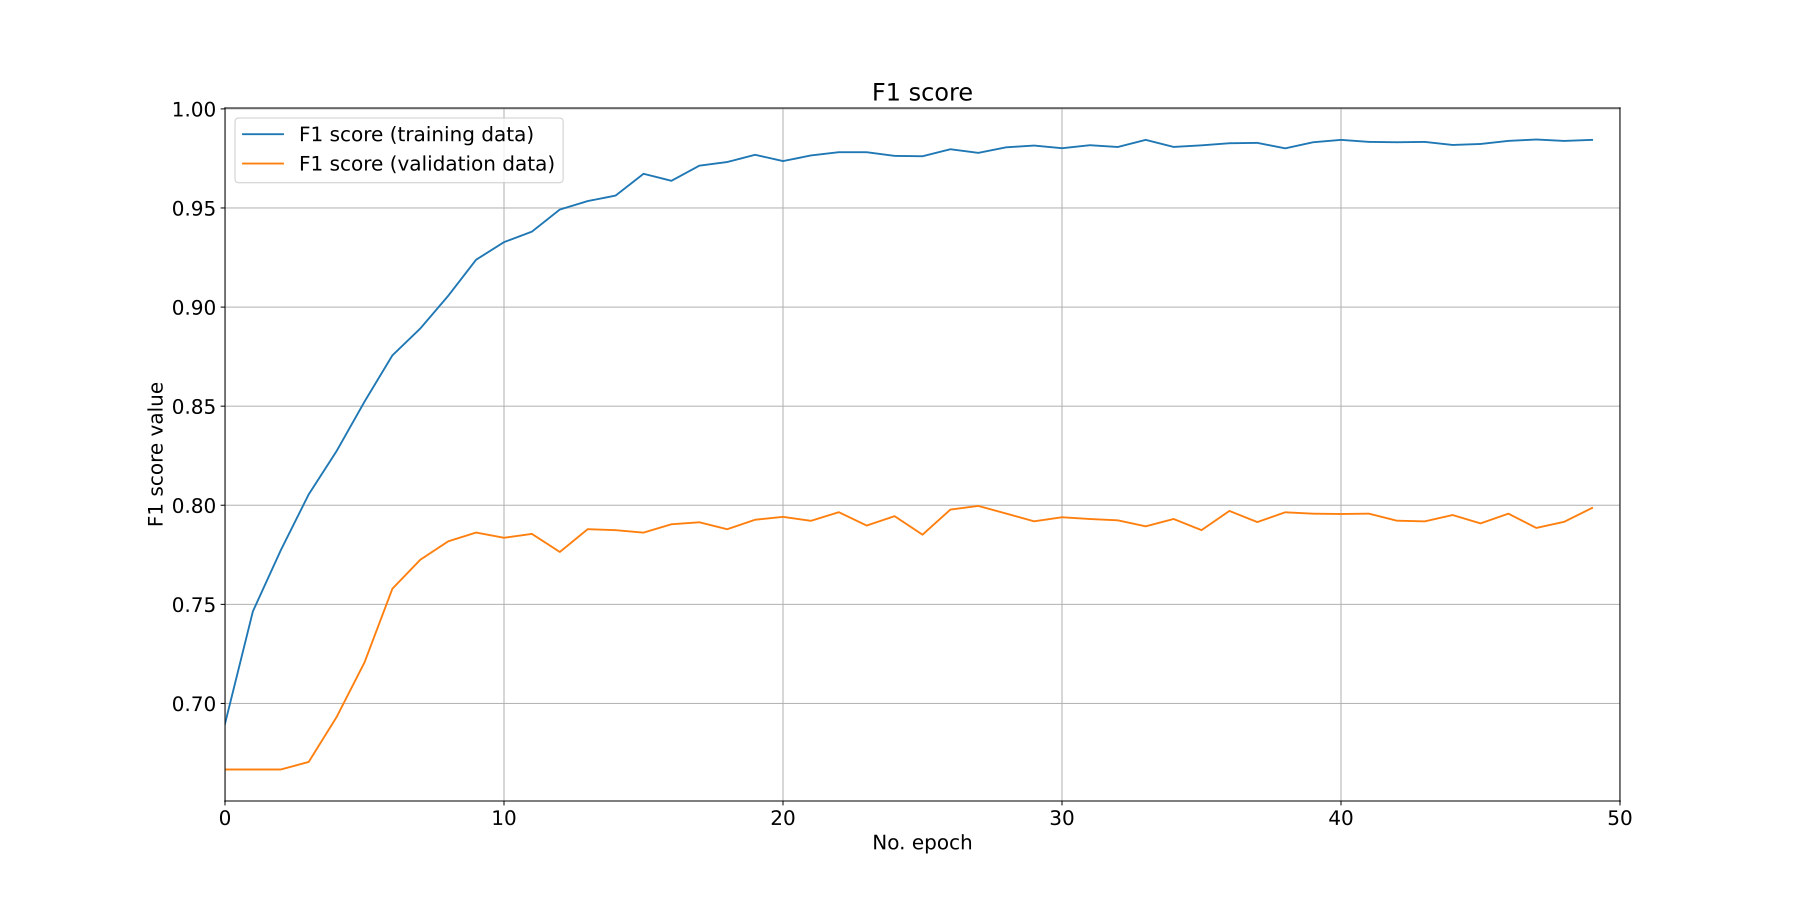
\includegraphics[width=80mm]{Figures/Sheffield/Sheffield_convolution_2d_f1_score_paper.png}}
	\subfloat[][Entrenamiento GTAAF en Cornwall]{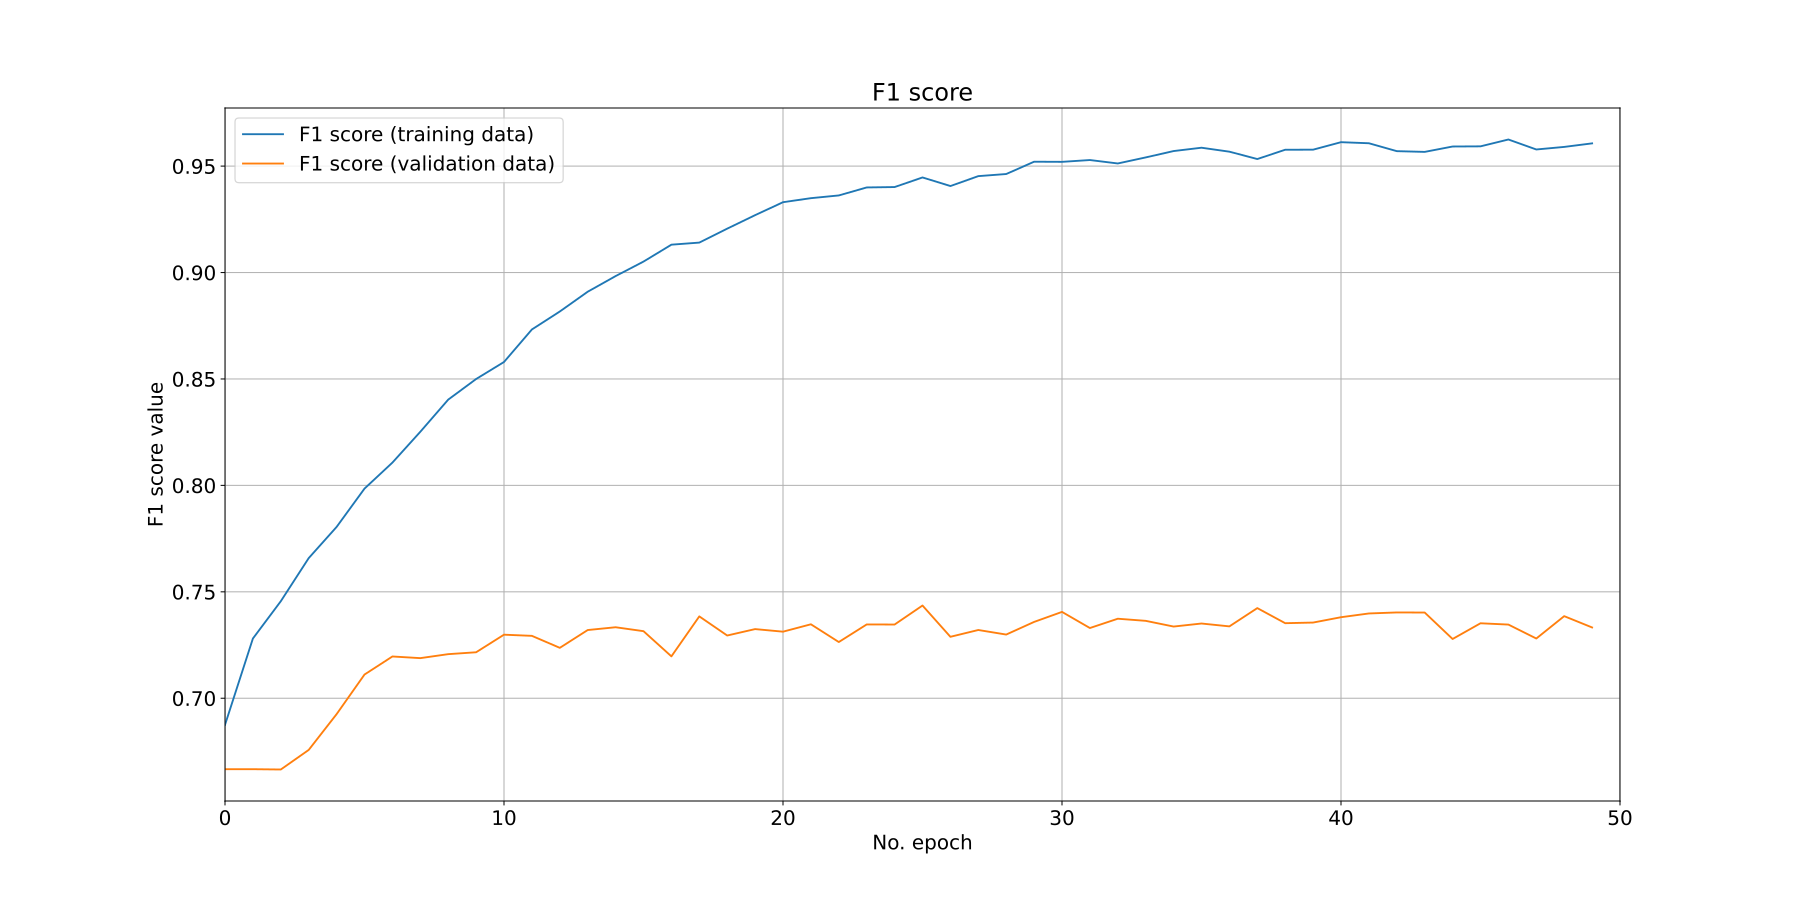
\includegraphics[width=80mm]{Figures/Cornwall/Cornwall_convolution_2d_f1_score_paper.png}}\\
	\caption{Evolución de \textit{F1-Score} del modelo GTAAF en las poblaciones de Reino Unido}
	\label{UKLossFunction}
\end{figure}


En la Tabla \ref{UKMetrics} se muestra el valor \textit{F1-Score} para cada una de las ciudades de cada modelo sobre el conjunto de test. Como se puede observar, el nuevo modelo propuesto GTAAF es el que mejor métricas ofrece en comparación al resto, obteniendo la mayor diferencia con respecto a su sucesor en los accidentes \textbf{Sin Asistencia}, el \textit{MLP}, para la ciudad de Manchester con un 6,7\%, mientras que la mayor diferencia para los accidentes \textbf{Con Asistencia} es de un 13.8\% en la ciudad de Southwark respecto al siguiente mejor modelo, de nuevo el \textit{MLP}. La siguiente mayor diferencia se presenta entre el modelo GTAAF se presenta en la ciudad de Southwark para la clase sin necesidad de asistencia, con un incremento del 4,8\% respecto al siguiente mejor modelo \textit{MLP}, mientras que para la clase con necesidad de asistencia ésta se presenta en la ciudad de Liverpool con respecto al modelo \textit{MLP}, llegando a un 13,2\%. Observando los resultados de la tabla, se aprecia que el mayor incremento del rendimiento con respecto al resto de modelos se presenta sobre la clase con necesidad de asistencia, obteniendo de media una mejora de 9,21\% sobre todas las ciudades, mientras que el incremento de rendimiento se acentúa menos en accidentes Sin Asistencia, ya que el resto de modelos ofrecen unas métricas más altas, siendo la mejora de un 3,93\% de media. Estos resultados reflejan una mejor generalización del modelo propuesto en comparación al resto de modelos estudiados para cada una de las ciudades de Reino Unido.

\begin{table}[H]
	\caption{\textit{F1-Score} por modelo y clase de accidente para cada una de las poblaciones de Reino Unido}
	\begin{center}
		\begin{tabular}{|c|c||c|c|c|c|c|c|}
			\hline
			\small
			\multicolumn{2}{ |c|| }{} &
			\multicolumn{6}{ |c| }{\textbf{\textit{F1-Score} Reino Unido}} \\ \hline
			
			\textbf{Modelo} & \textbf{Asistencia} & Southwark & Manchester & Birmingham & Liverpool & Sheffield & Cornwall
			\\ \hline \hline
			
			\multirow{2}{*}{NB} &
			No & 0.504 & 0.675 &  0.567 & 0.560 & 0.620 & 0.653 \\ &
			Sí & 0.400 & 0.482 & 0.558 & 0.417 & 0.669 & 0.484 \\ \hline \hline
			\multirow{2}{*}{SVC} &
			No & 0.826 & 0.845 & 0.812 & 0.865 & 0.809 & 0.702 \\ &
			Sí & 0.599 & 0.624 & 0.673 & 0.630 & 0.773 & 0.626 \\ \hline \hline
			\multirow{2}{*}{KNN} &
			No  & 0.652 & 0.723 & 0.747 & 0.746 & 0.754 & 0.656 \\ &
			Sí & 0.469 & 0.510 & 0.609 & 0.519 & 0.676 & 0.559 \\ \hline \hline
			\multirow{2}{*}{RF} &
			No & 0.561  & 0.118 & 0.303 & 0.742 & 0.313 & 0.711 \\ &
			Sí & 0.430 & 0.379 & 0.509 & 0.504 & 0.585 & 0.581 \\ \hline \hline
			\multirow{2}{*}{LR} &
			No & 0.711 & 0.800 & 0.761 & 0.806 & 0.733 & 0.630 \\ &
			Sí & 0.415 & 0.540 & 0.604 & 0.530 & 0.652 & 0.598 \\ \hline \hline
			\multirow{2}{*}{MLP} &
			No & 0.916 &  0.857 & 0.819 & 0.910 & 0.853 & 0.709 \\ &
			Sí & 0.743 & 0.632 & 0.662 & 0.721 & 0.810 & 0.671 \\ \hline \hline
			\multirow{2}{*}{\textbf     {GTAAF}} &
			\textbf{No} & \textbf{0.964} & \textbf{0.924} & \textbf{0.858} & \textbf{0.956} & \textbf{0.918} & \textbf{0.722} \\ &
			\textbf{Sí} & \textbf{0.881} & \textbf{0.762} & \textbf{0.711} & \textbf{0.853} & \textbf{0.889} & \textbf{0.707} \\ \hline \hline
		\end{tabular}
	\end{center}

	\label{UKMetrics}
\end{table}


La Figura \ref{GlobalSlightF1Score} muestra a modo de comparativa el rendimiento del nuevo modelo GTAAF propuesto en los accidentes \textbf{Sin Asistencia} para cada una de las poblaciones estudiadas respecto al resto de modelos del estado del arte con los que se ha experimentado en esta investigación. Se aprecia un incremento de rendimiento independientemente de las características individuales en todas las poblaciones respecto al resto de modelos estudiados, siendo el mayor incremento en la población de Victoria con un aumento del 6.5\% respecto al siguiente mejor modelo, el \textit{SVC}.

\begin{figure}[H]
	\centering
	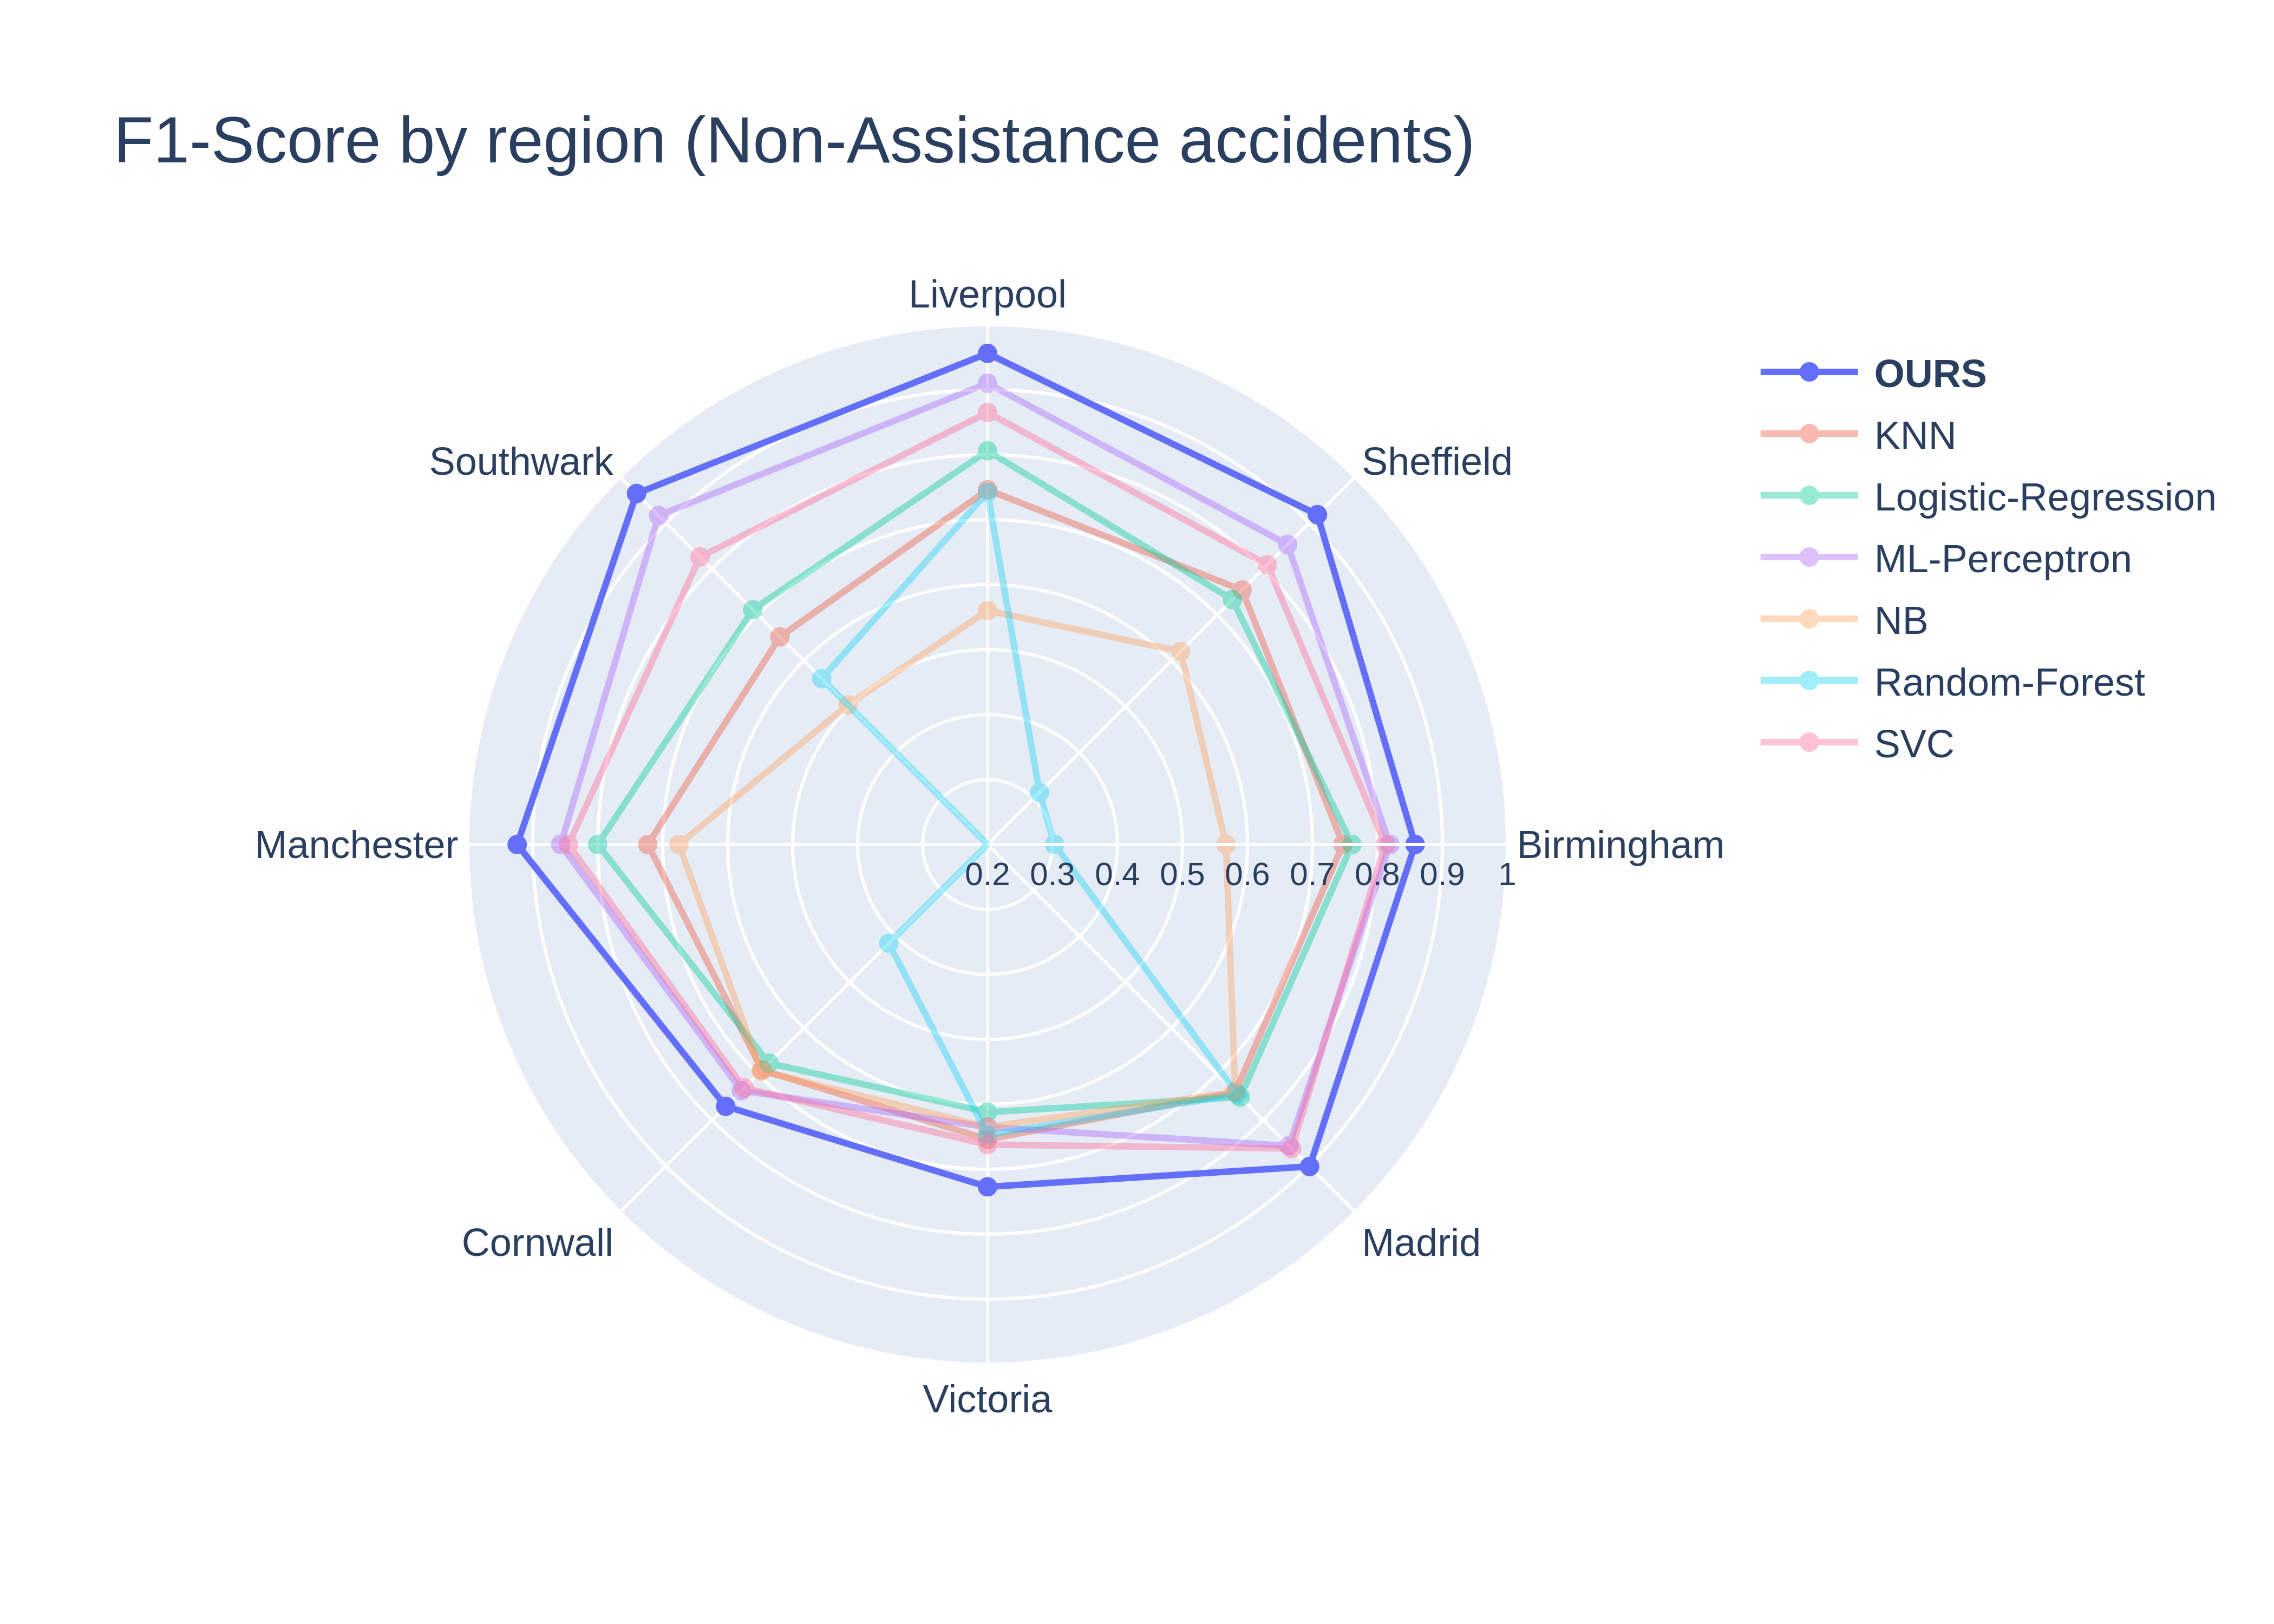
\includegraphics[width=150mm]{Figures/Slight.png}
	\caption{Comparación de \textit{F1-Scores} para accidentes Sin Asistencia (GTAAF)}
	\label{GlobalSlightF1Score}
\end{figure}

La Figura \ref{GlobalAssistanceF1Score} muestra la comparativa del rendimiento basado en el F1-Score de los modelos para cada una de las ciudades en los accidentes \textbf{Con Asistencia}. En esta gráfica se puede observar una diferencia considerablemente mayor del nuevo modelo GTAAF. La mayor mejora se presenta en la ciudad de Southwark, con un incremento del \textit{F1-Score} del 13.8\% respecto al siguiente mejor modelo sobre esta población, el \textit{MLP}.

\begin{figure}[H]
	\centering
	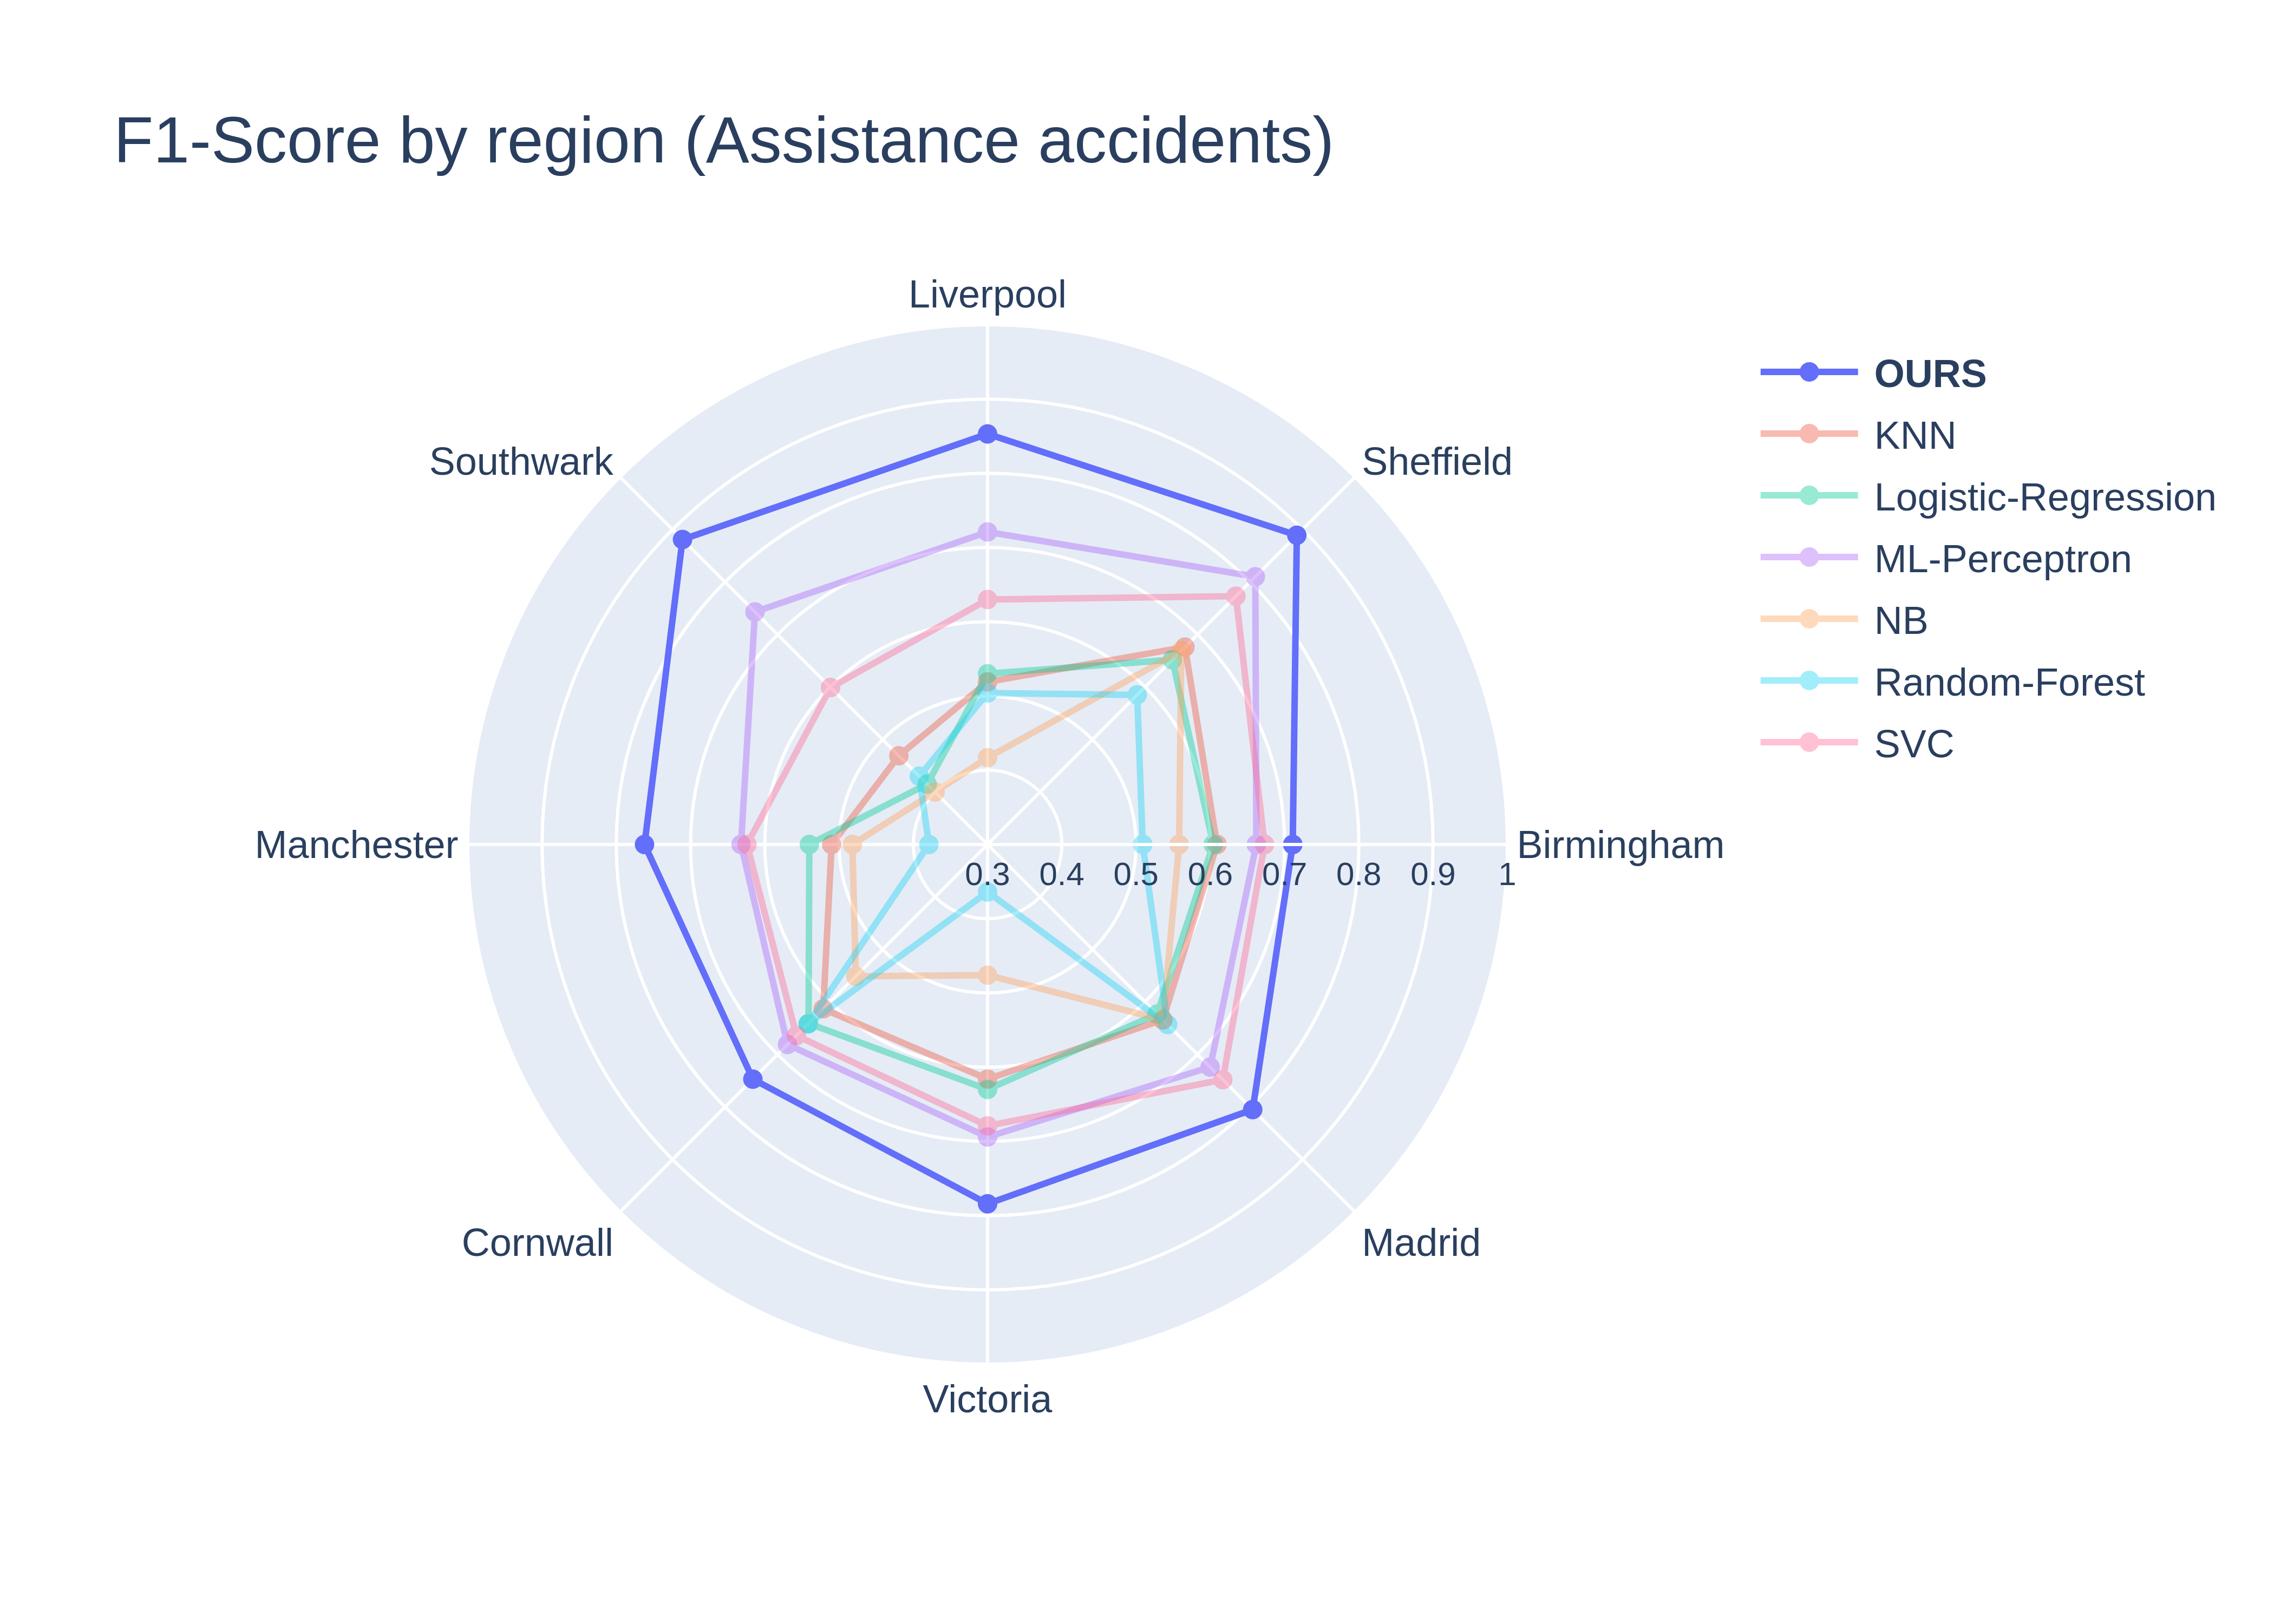
\includegraphics[width=150mm]{Figures/Assistance.png}
	\caption{Comparación de \textit{F1-Scores} para accidentes Con Asistencia (GTAAF)}
	\label{GlobalAssistanceF1Score}
\end{figure}

\subsection{Pruebas de robustez}


En esta sección se realizarán distintas pruebas de estrés. El objetivo de estas pruebas es medir el rendimiento del modelo propuesto en casos extremos utilizando como base los conjuntos de datos expuestos en esta tesis para tener una aproximación del rendimiento del modelo en futuros conjuntos de datos que no dispongan de la totalidad de las características descritas en este documento. Para ello se realizarán tres experimentos para cada conjunto de datos, estos consistirán en eliminar aquellas variables de mayor y menor importancia de forma independiente, y, en un experimento posterior, se eliminarán ambas conjuntamente con el objetivo de medir el rendimiento ante la falta de características más y menos influyentes en futuros conjuntos de datos. La evaluación de la importancia de las características viene dada por el peso asignado a cada una de estas mediante el algoritmo \textit{XGBoost} optimizado mediante el algoritmo genético.

% \textcolor{orange}{\textbf{LUIS: Copiado y pegado del paper 3}}

Como se puede intuir en la Figura \ref{FeaturesClassification}, uno de los principales problemas en la generalización de un modelo es la disponibilidad de datos. Existen distintas características disponibles en cada conjunto de datos por distintos motivos. Uno de ellos puede ser la dificultad de extracción de información debido a razones económicas, sociales o políticas. Por ejemplo, tenemos el caso extremo de Madrid, que perdió toda una categoría (Driving Limitations)

Necesitamos probar la robustez y generalización de la metodología y el modelo descritos en esta investigación. Con este propósito, proponemos el tercer experimento: eliminar las variables que tienen la mayor y menor importancia para cada población basándonos en la importancia de cada característica durante el entrenamiento del algoritmo de impulso. Específicamente, se llevaron a cabo tres experimentos independientes para ambas poblaciones. El primero consistió en eliminar la variable con la menor importancia dentro de los datos, el segundo en eliminar la de mayor importancia, y el tercero en eliminar ambas simultáneamente.

Esta prueba de robustez se realizó en dos poblaciones: Cornwall (Reino Unido) y la población de Victoria, con el objetivo de simular nuevos conjuntos de datos donde no estén disponibles todos los datos mencionados en este documento.

En este análisis de resultados (consulte las Tablas \ref{CornwallLoss} y \ref{Victorialoss}), comparamos la brecha de rendimiento entre el nuevo modelo GTAAF propuesto y el mejor modelo posterior para cada experimento. Además, evaluaremos la diferencia en la métrica de F1-Score obtenida en comparación con los resultados presentados en secciones anteriores donde estas características estaban presentes.

%%%%%%%%%%%%%%%%%%%%%%%%%%%%%%%%%%%%%%%%%%%%%%%%%%%%%%%%%%%%%%%%%%%%%%%%%%%%%%%%%
\begin{table}[H]
	\caption[Comparativa \textit{F1-Score} con eliminación de características sobre Cornwall. Modelo GTAAF]{Comparativa \textit{F1-Score} con eliminación de características sobre Cornwall. Modelo GTAAF. La columna \textit{Menor} representa los resultados obtenidos ejecutando el modelo y eliminando la característica que menor peso presenta mediante el algoritmo genético, la columna \textit{Mayor} presenta los resultados eliminando la característica de mayor importancia y \textit{Ambas} presenta los resultados eliminando las dos simultáneamente. En negrita se muestran los resultados obtenidos por el mejor modelo (GTAAF)}
	\begin{center}
		\begin{tabular}{|c|c||c|c|c|c|c|c|}
			\hline
			\multicolumn{2}{ |c|| }{} &
			\multicolumn{3}{ |c| }{\textbf{Cornwall}} \\ \hline
			
			\textbf{Modelo} & Asistencia & Menor & Mayor & Ambas
			\\ \hline \hline
			
			\multirow{2}{*}{NB} &
			No & 0.668 & 0.597 & 0.592\\ &
			Sí  & 0.490 & 0.535 & 0.519 \\ \hline \hline
			\multirow{2}{*}{SVC} &
			No & 0.710 & 0.631 & 0.646\\ &
			Sí  & 0.628 & 0.626 & 0.620 \\ \hline \hline
			\multirow{2}{*}{KNN} &
			No & 0.671 & 0.601 & 0.637\\ &
			Sí  & 0.571 & 0.532 & 0.559 \\ \hline \hline
			\multirow{2}{*}{RF} &
			No & 0.719 & 0.498 & 0.514\\ &
			Sí  & 0.603 & 0.638 & 0.644 \\ \hline \hline
			\multirow{2}{*}{LR} &
			No & 0.670 & 0.575 & 0.567\\ &
			Sí  & 0.626 & 0.585 & 0.580 \\ \hline \hline
			\multirow{2}{*}{MLP} &
			No & 0.724 & 0.652 & 0.680\\ &
			Sí  & 0.695 & 0.654 & 0.685 \\ \hline \hline
			\multirow{2}{*}{\textbf{GTAAF}} &
			No & \textbf{0.768} & \textbf{0.736} & \textbf{0.792}\\ &
			Sí  & \textbf{0.766} & \textbf{0.736} & \textbf{0.787} \\ \hline \hline
		\end{tabular}
	\end{center}

	\label{CornwallLoss}
\end{table}
%%%%%%%%%%%%%%%%%%%%%%%%%%%%%%%%%%%%%%%%%%%%%%%%%%%%%%%%%%%%%%%%%%%%%%%%%%%%%%%%%


%%%%%%%%%%%%%%%%%%%%%%%%%%%%%%%%%%%%%%%%%%%%%%%%%%%%%%%%%%%%%%%%%%%%%%%%%%%%%%%%%
\begin{table}[H]
	\caption[Comparativa \textit{F1-Score} con eliminación de características sobre Victoria. Modelo GTAAF]{Comparativa \textit{F1-Score} con eliminación de características sobre Victoria. Modelo GTAAF. La columna \textit{Menor} representa los resultados obtenidos ejecutando el modelo y eliminando la característica que menor peso presenta mediante el algoritmo genético, la columna \textit{Mayor} presenta los resultados eliminando la característica de mayor importancia y \textit{Ambas} presenta los resultados eliminando las dos simultáneamente. En negrita se muestran los resultados obtenidos por el mejor modelo (GTAAF)}
	\begin{center}
		\begin{tabular}{|c|c||c|c|c|c|c|c|}
			\hline
			\multicolumn{2}{ |c|| }{} &
			\multicolumn{3}{ |c| }{\textbf{Victoria}} \\ \hline
			
			\textbf{Modelo} & Asistencia & Menor & Mayor & Ambas
			\\ \hline \hline
			
			\multirow{2}{*}{NB} &
			No & 0.639 & 0.613 & 0.607\\ &
			Sí  & 0.465 & 0.553 & 0.572 \\ \hline \hline
			\multirow{2}{*}{SVC} &
			No & 0.653 & 0.638 & 0.664\\ &
			Sí  & 0.657 & 0.650 & 0.676 \\ \hline \hline
			\multirow{2}{*}{KNN} &
			No & 0.625 & 0.627 & 0.638\\ &
			Sí  & 0.540 & 0.562 & 0.566 \\ \hline \hline
			\multirow{2}{*}{RF} &
			No & 0.630 & 0.630 & 0.621\\ &
			Sí  & 0.248 & 0.161 & 0.071 \\ \hline \hline
			\multirow{2}{*}{LR} &
			No & 0.598 & 0.574 & 0.599\\ &
			Sí  & 0.609 & 0.637 & 0.646 \\ \hline \hline
			\multirow{2}{*}{MLP} &
			No & 0.635 & 0.636 & 0.654\\ &
			Sí  & 0.693 & 0.686 & 0.692 \\ \hline \hline
			\multirow{2}{*}{\textbf{GTAAF}} &
			No & \textbf{0.732} & \textbf{0.720} & \textbf{0.778}\\ &
			Sí  & \textbf{0.780} & \textbf{0.793} & \textbf{0.814} \\ \hline \hline
		\end{tabular}
	\end{center}

	\label{Victorialoss}
\end{table}
%%%%%%%%%%%%%%%%%%%%%%%%%%%%%%%%%%%%%%%%%%%%%%%%%%%%%%%%%%%%%%%%%%%%%%%%%%%%%%%%%

En este experimento es necesario destacar un resultado: en nuestra propuesta, el modelo GTAAF, existe una gran mejora sobre los resultados del mismo modelo con todas las características. En contraste, hay un gran deterioro en los resultados de los otros modelos con los que se compara. En otras palabras, la diferencia en la puntuación \textit{F1-Score} entre GTAAF y los otros modelos aumenta. Esta circunstancia sugiere que nuestro modelo se ve afectado por las características extremas, donde el modelo de \textit{XGBoost} y el algoritmo genético favorecen y desfavorecen las características más y menos relevantes. Este no es el caso para los otros algoritmos, donde todas las características son individualizadas.

En la Figura \ref{lossFig} podemos observar la diferencia de los algoritmos con y sin pérdida de características (Tablas \ref{UKMetrics}, columna Cornwall, y \ref{AustraliaMetrics} contra las Tablas \ref{CornwallLoss} y \ref{Victorialoss} respectivamente). Mostramos cómo nuestro modelo mejora sus propios resultados en todos los casos. Por ejemplo, en Cornwall, obtenemos una mejora en nuestro modelo del 4.8\% y 5.9\% en los accidentes \textbf{Sin Asistencia} y \textbf{Con Asistencia} (eliminando la peor característica, ver la barra azul en la Figura \ref{lossFig}-arriba), 1.4\% y 2.9\% (eliminando la mejor característica, ver la barra verde en la Figura \ref{lossFig}-arriba) y 7\% y 8\% (eliminando ambas características, ver la barra gris en la Figura \ref{lossFig}-arriba), respectivamente. Evaluando un área más dispersa como Victoria, los resultados son similares pero con una mejora menor: 0.5\% y 0.4\% (ver la barra azul en la Figura \ref{lossFig}-abajo), -0.7\% y 0.9\% (ver la barra verde en la Figura \ref{lossFig}-abajo), y 5.1\% y 3\% (ver la barra gris en la Figura \ref{lossFig}-abajo), respectivamente. Esto indicaría un efecto menor de los valores extremos en la ponderación del algoritmo genético si el área es más dispersa.

\begin{figure}[H]
	\centering
	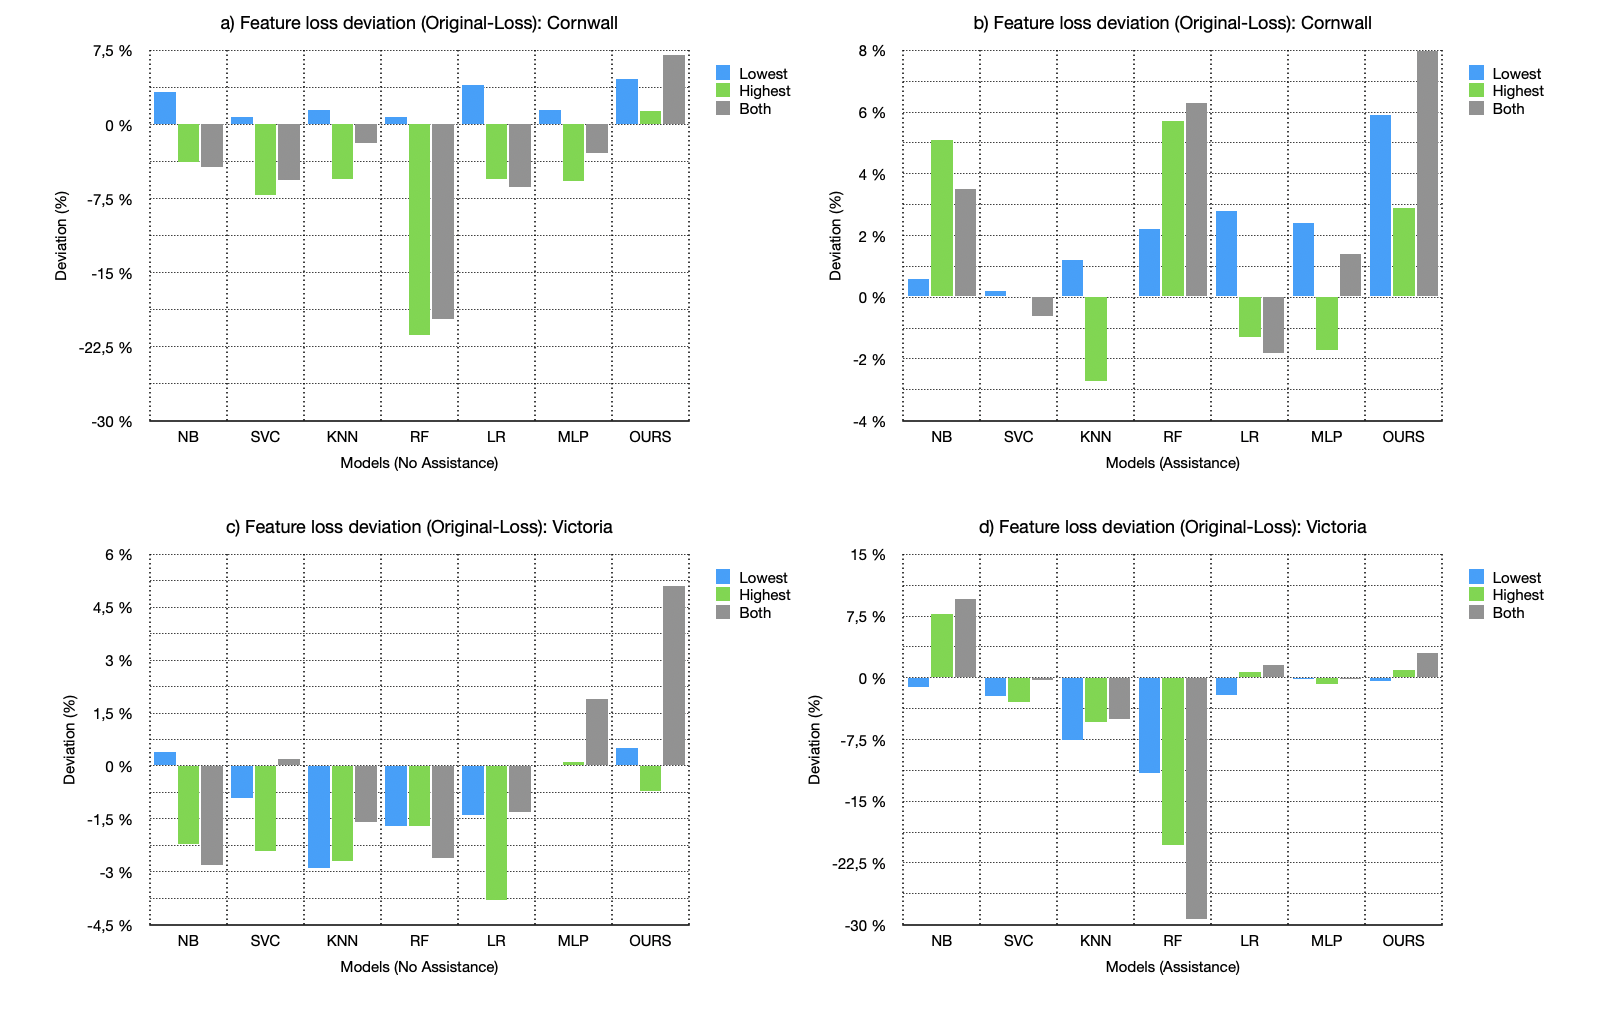
\includegraphics[width=150mm]{Figures/LossFeatures/loss.png}
	\caption[Comparación de pérdida de características del modelo GTAAF]{Comparación de pérdida de características del modelo GTAAF. Las barras representan la diferencia entre los resultados con todas las características y los resultados sin características extremas: en azul sin la característica más baja, en verde sin la característica más alta y en gris sin ambas características extremas}
	\label{lossFig}
\end{figure}

